

\documentclass[12pt]{book}

\usepackage[italian]{babel}

\usepackage[paperwidth=5.5in,paperheight=8.5in]{geometry}

%\usepackage[a4,frame,center]{crop}

\usepackage[autostyle]{csquotes}
\usepackage{epigraph}

\usepackage[hidelinks]{hyperref}
%\hypersetup{colorlinks=true,urlcolor=blue}
\usepackage{nameref}

\usepackage{pdfpages}

\usepackage{qrcode}

\usepackage{poetry}

\usepackage{amsmath}
%\usepackage{amsthm}
%\usepackage{amssymb}
%\usepackage{mathrsfs}
\usepackage{amsfonts}


% \usepackage{verbatim}

\poemlinenumsfalse
\newenvironment{vcentered}{
    \pagebreak
    \topskip0pt
    \vspace*{\fill}
}{
    \vspace*{\fill}
    \pagebreak
}

\newenvironment{haiku}{
    \begin{vcentered}
    \begin{poem}
}{
    \end{poem}
    \end{vcentered}
}

\newenvironment{haikuSimple}{
    \begin{poem}
}{
   \end{poem}
   \leavevmode\\ 
   \leavevmode\\ 
}


\let\urlOrig\url
\def\url#1{\urlOrig{#1} \qrcode{#1}}


\usepackage{amsthm}

%\newtheorem{thm}{Theorem}[section]
\theoremstyle{definition}
\newtheorem{definizione}{Definizione}



%%
%\usepackage[landscape]{geometry}
%%

%\usepackage{xr-hyper}


%\usepackage{amsmath}
%\usepackage{amsthm}
%\usepackage{amssymb}
%\usepackage{mathrsfs}
%\usepackage{amsfonts}
%

\newtheorem{thm}{Theorem}[section]
\newtheorem{exemp}[thm]{Example}
\newtheorem{defn}[thm]{Definizione}


\usepackage[it-IT]{datetime2}

\def\finishDate{\DTMdate{2021-10-22}}


\usepackage{graphicx}


\newcommand{\eal}[1]{{\begin{align*} #1 \end{align*}}}
\def\nl{{\\&\qq }} % newline inside \eal{}
\def\NN{\\& } % newline inside \eal{}

\def\Diomath{\mathcal{D}\textrm{io}}

\def\lastUpdateDate{\DTMdate{2025-09-08}}

\begin{document}

%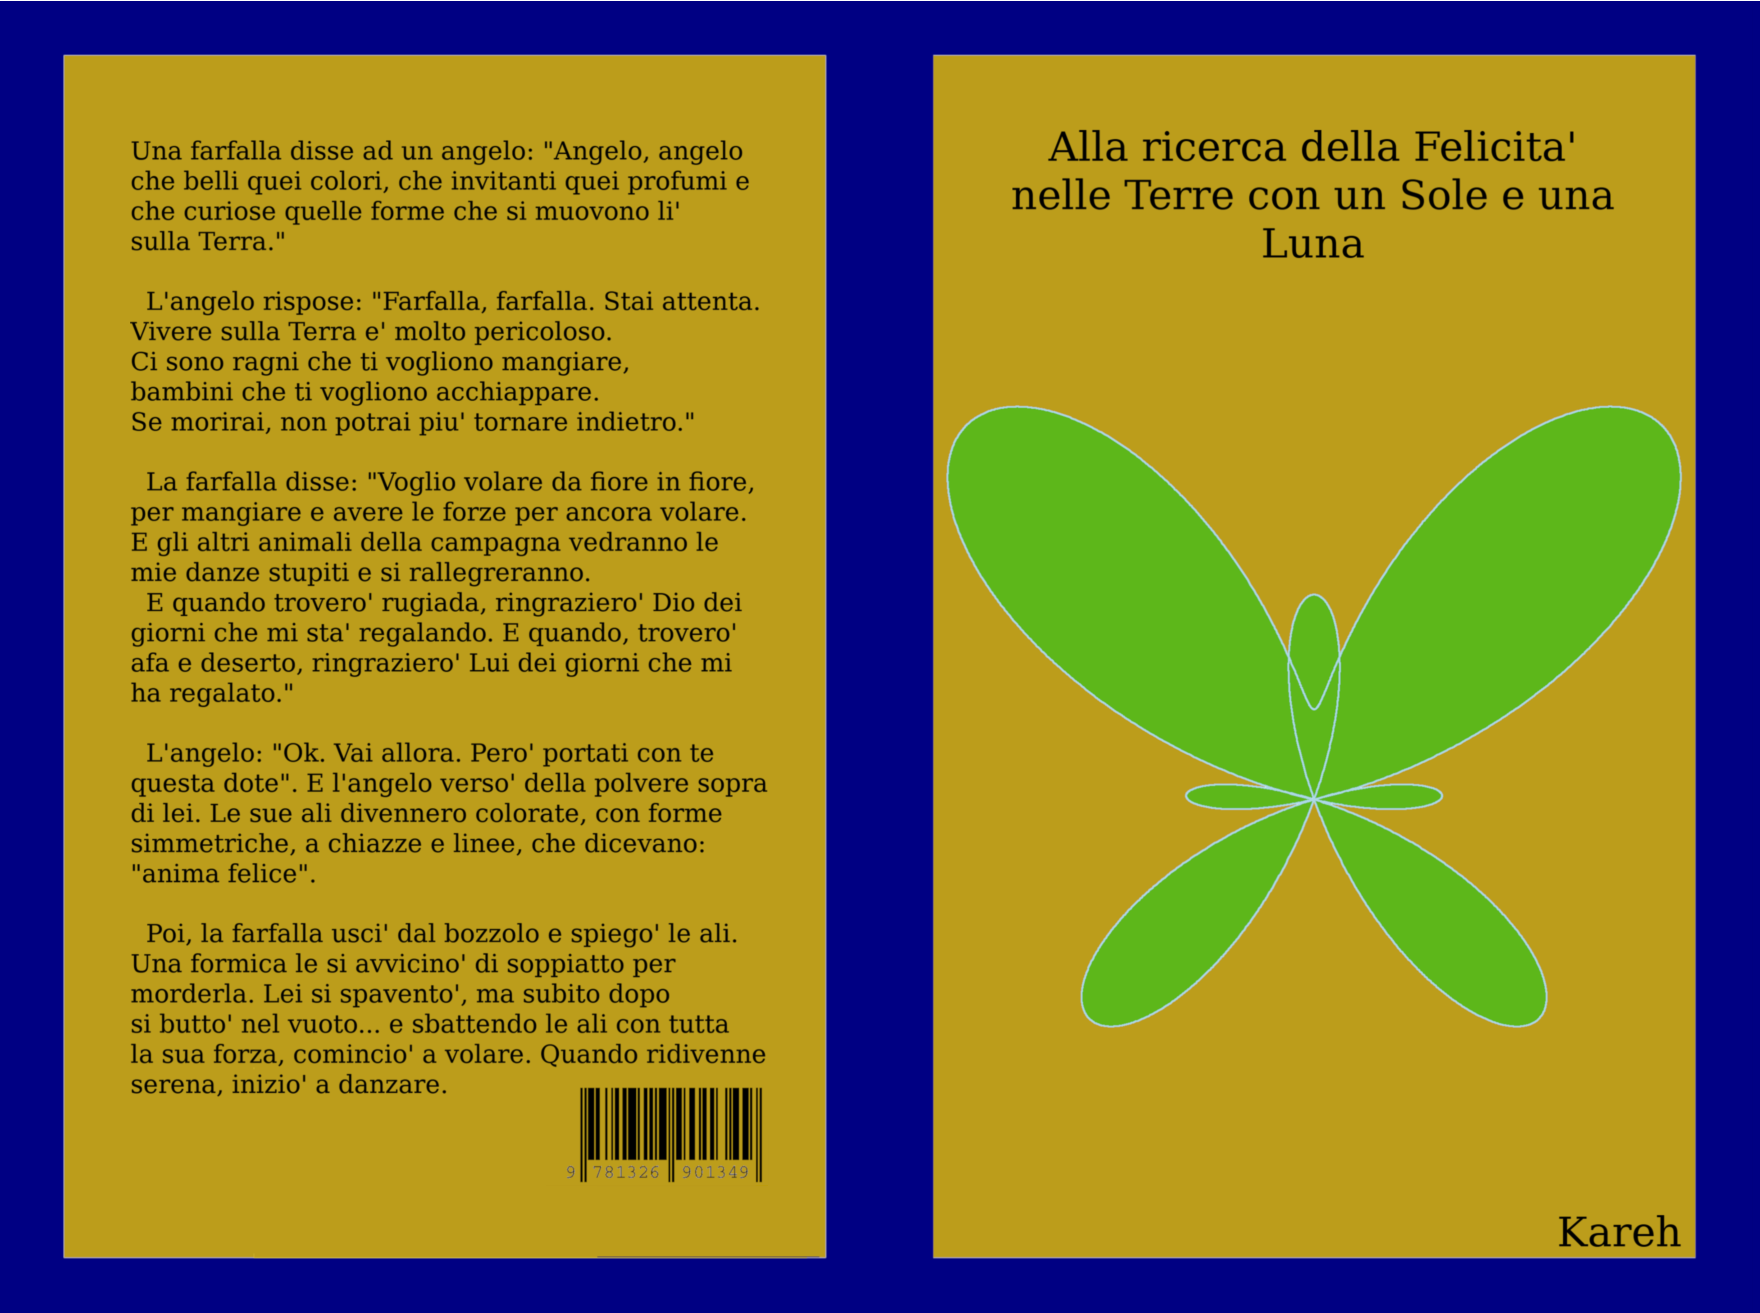
\includepdf[fitpaper]{cover/cover.pdf}

\title{
    Alla ricerca della Felicita'\\
    nelle Terre con un Sole e una Luna
}

\date{}

\maketitle{}

\frontmatter



\leavevmode\\
\small{\textcopyright} Kareh \\
\leavevmode\\

\vfill

Tutti i testi e le immagini sono dedicati al pubblico dominio, secondo la licenza Creative Commons ``CC0 1.0 Universal (CC0 1.0) Donazione al Pubblico Dominio''.

Puoi copiare, modificare, distribuire ed utilizzare l'opera, anche per fini commerciali, senza chiedere alcun permesso.

Per maggiori informazioni: \url{https://creativecommons.org/publicdomain/zero/1.0/deed.it}

\leavevmode\\
\leavevmode\\
\leavevmode\\

\begin{flushright}
    ISBN: 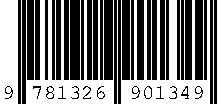
\includegraphics{lulu/isbn/978-1-326-90134-9.pdf}
\end{flushright}


\tableofcontents

\chapter{Prefazione}
Da ragazzo sapevo che esisteva qualcosa oltre la monota routine della scuola, dei compiti, delle esauste battute e dei logori scherzi tra compagni. Cosi', mi ero messo a cercare la ``vita vera'' nell'informatica e nella matematica, dove, ogni giorno che passava, conoscevo cose arcane e stupende. Ma non sarebbe bastata tutta la conoscenza di Eulero ed Erdos per parlare al mio cuore della vera vita. Ne' era poi cosi' difficile avvicinarsi ad essa. Bastava ``arrendersi a Dio'' e mettersi in gioco per quanto la propria ed altrui anima chiedeva. Oggi, dopo venti anni, capisco com'e' la ``vita vera''. Non l'ho pienamente raggiunta, ma la capisco e, con il costo di costanti piccoli e grandi impegni e sacrifici, la amo sempre piu'.


La vita vera esiste. Ce ne ricordiamo quando leggiamo un bel libro, che ci coinvolge e ci guida lungo una riflessione, lungo un viaggio.  La vita vera e' contenuta dentro di noi. Non occorre andare ad abitare lontano, conquistare un titolo altisonante od ottenere gli oggetti dei propri desideri. E' sufficiente diventare grandi, senza dover essere super-man. Fermarsi e fare un dono a chi e' piu' piccolo, nonostante si stia attraversando un periodo stressante, e' lo stesso gesto di un eroe che, nonostante sia dedito e preoccupato per la sua rischiosa impresa, si ferma nel suo cammino per esaudire il desiderio di un bambino.

Raggiungere la vera vita e', tuttavia, l'impresa piu' difficile, stressante e piu' lunga che si possa immaginare. Praticamente nessuno sa' come raggiungerla, altrimenti il mondo sarebbe gia' in Pace, ma ognuno e' in grado di mettersi in cammino per trovarla, di impegnarsi per costruirla, di pazientare per coltivarla.

Un esempio, e' cercare la vera vita nel lavoro.

Chi ricerca la vera vita lavorando, si alza anche la ventesima mattina, dopo averlo fatto gia' 19 giorni nello stesso mese, e va a lavorare, nonostante farebbe bene al suo fegato fare una semplice passeggiata dal fruttivendolo o
stringere la mano del suo amore e stare cosi' una mezz'ora.

Andare a lavoro perche' 
\begin{enumerate}
    \item il proprio capo probabilmente non capirebbe, dato che non ha cognizione delle nostre esigenze. E avere cognizione delle esigenze di ogni dipendente non e' una cosa facile ed e' molto impegnativa.
    \item Perche', noi non abbiamo cognizione completa dei piani dei nostri capi e di quello che stanno facendo i colleghi. Delle difficolta' che sta' affrontando l'azienda, di quello che vuole fare per il prossimo futuro.\\
        Magari piu' o meno lo sappiamo, ma non sappiamo nel dettaglio le cose, e nel lavoro i dettagli sono fondamentali.\\
        Se potessimo farlo e ci assentassimo o ritardassimo a nostro arbitrio, 
        e se lo facessero tutti i dipendenti, piu' spesso mancherebbe la persona che proprio quel giorno serve, e cosi' la produttivita' calerebbe.
    \item Perche' molti clienti, ad ogni minimo calo di qualita' od aumento del costo passerebbero subito ad altre aziende.
    \item Perche' le altre aziende non aspettano altro che un momento debole della nostra azienda per superla e prendere la sua fetta di mercato.
\end{enumerate}
Andando a lavorare credendo in quello che si fa, si ha la possibilita' di stare con altre persone, che come noi cercano di sopravvivere impegnandosi; di rinforzare la fiducia in noi stessi tramite i piccoli quotidiani successi; di conoscere persone diverse da noi, al di fuori del nostro cerchio di amicizie.\\
Di stare con i colleghi ed avere la possibilita' di trasmettere le proprie tecniche e i propri trucchi, di mettersi a disposizione delle loro piccole difficolta'.\\
Di sopportare chi ci e' antipatico, perche' noi in tutta la nostra vita abbiamo fatto di tutto per fare tacere quelle parti del vivere che, invece, a nostro avviso, lui lascia totalmente libere o vizia. E poi, rendersi conto che, in realta', il suo modo di vivere ci interessa sotto certi aspetti, e che ne' continuando ad essere come noi siamo, ne' essendo esattamente come lui e' arriveremo alla Meta. E, capito cio', cambiando nel tempo, ritrovare la pace di stare con lui.\\
Di impegnarsi su problemi che solo noi sappiamo o dobbiamo risolvere. Ricorrere a tutta la propria esperienza, resistenza e astuzia. Paura, poi fede, speranza, poi impegno e ancora impegno, e pazienza e ancora impegno, e poi il momento fatidico della messa in atto, e poi il successo. La gioia con i colleghi, le lodi del capo. E poi, l'indomani, la solita routine :)\\
Di tornare la sera, sapendo di aver fatto di meglio che si poteva nella giornata per se stessi e per tutti, mangiare un piatto semplice e nutriente, parlare con chi si vive con le poche forze che si hanno, chiudere gli occhi e ritornare nella nostra dimora fuori dal tempo e dello spazio.\\

Non esiste solo il lavoro. Esistono molti altri modi per ricercare la vera vita: la maestria nell'arte, o nella tecnica, o nello sport o nella scienza; la ricerca e la coltivazione dell'amore; la tranquillita' nella famiglia e la sua protezione.\\

Per quanto difficile o inauspicabile, accettare, curare e amare la propria e altrui vita, qualunque sia il punto di partenza e' la vera vita.\\

Il piacere della vita vera e' ineguagliabile.\\
E' genuino e ricco, e' raffinato e inarrestabile.\\

Vedere e sentire che la propria o altrui vita cresce e poi fiorisce e' il piacere piu' grande.
Tutti gli altri piaceri sono declinazioni di questo.\\

Chi capisce e nutrisce nel tempo questa consapevolezza, impara ad amare se stesso e gli altri,

\centerpoemon{senza aspettare soldi,}
\begin{poem}
a mani nude,\\
senza aspettare soldi,\\
assistenza,\\
luoghi, occasioni,\\
altro.\\
\end{poem}

\leavevmode\\
Per ogni persona che si alza per ricercare la vera vita,
la vita di tutti migliora esponenzialmente.\\

Questi racconti, poesie e pensieri, sono tracce dei risultati che ho raggiunto con i miei sforzi, con il contributo e con l'affetto di chi mi e' stato vicino.\\
Vogliono essere una piccola dimostrazione dell'esistenza della vera vita.

\begin{flushright}
    \vspace*{\fill}
    Kareh, \finishDate
\end{flushright}


\section{Links}

Pagina web del libro:\\
\url{https://kareh.github.io}\\

\leavevmode\\
Codice sorgente (LaTeX):\\
\url{https://github.com/kareh/ricercafelicita}



\mainmatter

\chapter{Tracce sul cammino}

Poesie, inizialmente ispirate agli Haiku zen, ognuna delle quali segna un punto del mio personale cammino, e del cammino che credo ognuno di noi compira', similmente.

\vfill

\centerpoemon{L'universo che ama,}
\begin{haiku}
L'universo,\\
infinito, freddo.\\
\leavevmode\\
L'amore,\\
caldo, limitato.\\
\leavevmode\\
Cosa altro cercare?\\
\end{haiku}


\begin{haiku}
Adattarsi \\
vuol dire\\
non forzare.\\
\end{haiku}

\centerpoemon{e piano, a volte inaspettatemente,}
\begin{haiku}
Dal lunedi' al venerdi',\\
in miniera lavoro.\\
\leavevmode\\
Sabato mattina,\\
il Sole acceca.\\
\leavevmode\\
Poi, il vento\\
mi riconduce al Suo amore,\\
e piano, a volte inaspettatamente,\\
un incantevole fiore sboccia.\\
\leavevmode\\
Con nuova forza,\\
lunedi' al lavoro!\\
\end{haiku}

\centerpoemon{per accogliere, accettare e non chiedere oltre}
\begin{haiku}
Il vero Guerriero\\
combatte solo con se stesso,\\
per annientare il suo ego.\\
\leavevmode\\
Per dare senza aspettare un grazie.\\
Per accogliere e ricevere solo\\
quello chi gli viene donato.\\
\leavevmode\\
Contento di cio' che esiste,\\
esalta le richezze delle terre piu' povere,\\
si rallegra delle virtu', piccole o grandi,\\
di chi incontra.\\
\end{haiku}

\centerpoemon{Con quattro giochi,}
\begin{haiku}
Con quattro giochi,\\
semplici e poveri,\\
felici.\\
\end{haiku}

\centerpoemon{
nuotando piano piano,
}
\begin{haiku}
La boa lontana,\\
nuotando piano piano,\\
si avvicina.\\
\end{haiku}

\centerpoemon{
la nostra vela viene facilmente spinta da
}
\begin{haiku}
Non perche' il sole e' molto grande,\\
noi siamo molto piccoli.\\
\leavevmode\\
Infatti, proseguendo nella grande rotta,\\
la nostra vela viene facilmente spinta da\\
un forte e sicuro vento,\\
generato da un grande sole.\\
\end{haiku}

\centerpoemon{di criptografia, implementano server e programmi}
\begin{haiku}
Il vero matematico e' colui che\\
crede che l'Amore esiste\\
e che vive per dimostrarlo.\\
\leavevmode\\
Nota: a volte, Egli (o Ella) e' un
matematico dei numeri, delle forme e delle regole\\
e dimostra teoremi per arrivare alla\\
stessa conclusione.\\
Ad esempio, Eulero con il suo teorema,\\
ha permesso ai matematici di capire meglio\\
la teoria dei numeri, e agli informatici\\
di ideare la criptografia R.S.A.\\
I programmatori, avvalendosi degli algoritmi\\
di criptografia, implementano server e programmi\\
sicuri, un esempio e' https, che protegge\\
il traffico web wifi, cosi' quando\\
noi ci logghiamo su un sito come Gmail o poste.it,\\
nessun ladro puo' captare la nostra password\\
con un antenna.\\
\end{haiku}

\centerpoemon{Cambiare allontandosi dal non stare bene,}
\begin{haiku}
    Amore: \\
    stare bene.\\
    Partendo da come si e',\\
    da come gli altri sono,\\
    da come l'ambiente e',\\
    per stare meglio.\\
    \leavevmode\\
    Da soli,\\
    con altri.\\
    Nel deserto,\\
    nella valle in fiore.\\
    \leavevmode\\
    Se non si sta' bene,\\
    cambiare, lavorare,\\
    camminando verso l'infinito bene.\\
    \leavevmode\\
    Volgere il proprio stare,\\
    affinche' anche gli altri\\
    stiano bene,\\
    ma ancora di piu',\\
    anche loro cerchino \\
    questo completo,\\
    autentico piacere.\\
    \leavevmode\\
    Per quanto stare e cambiare,\\
    sia difficile.\\
\end{haiku}

\centerpoemon{affinche' non smetta mai di esserlo.}
\begin{haiku}
    Sia Dio\\
    la personificazione\\
    dell'Amore.\\
    \leavevmode\\
    E la religione,\\
    l'emulare l'Amore\\
    tramite regole, pensieri, parole,\\
    fino a che il proprio respiro\\
    diventi Amore,\\
    affinche' non smetta mai di esserlo.\\
\end{haiku}

%\centerpoemon{Quando l'avrai fatto abbondantemente,}
%\begin{haiku}
%    Non lamentarti \\
%    per coloro che non vogliono cambiare. \\
%    \leavevmode \\
%    Fatica \\
%    per chi lo desidera. \\
%    \leavevmode \\
%    Quando l'avrai fatto abbondantemente,\\
%    chiediti: se cambiare, \\
%    vuol dire avvicinarsi a Lui,\\
%    chi non lo desidera ?\\
%    \leavevmode\\
%    E il tuo dolore, scomparso,\\
%    sara' comprensione e carita'.\\
%\end{haiku}



\centerpoemon{ Gli animali piu' semplici }
\begin{haiku}
    Gli animali\\
    piu' semplici,\\
    capiscono solo,\\
    se stanno bene o male.\\
    E questo li rende felici.\\
\end{haiku}

\centerpoemon{Non c'e' niente delle meraviglie della scienza}
\begin{haiku}
    Non c'e' niente delle meraviglie della scienza,\\
    sia fisiche, microscopiche o cosmische,\\
    sia psicologiche, emotive, individuali, collettive o globali,\\
    che eguagli la bellezza della religione,\\
    del consumare la vita,\\
    per il bene a cui la vita crede.\\
    \leavevmode\\
    Ma ogni meraviglia della scienza,\\
    ricorda la Verita' e indirizza a Lei:\\
    Dio vuole la vita,\\
    non la morte.\\
    \leavevmode\\
    Dio non ammette uno spreco\\
    di neanche un infinitesimo di vita.\\
    E se sulla terra il corpo si logora nel tempo,\\
    e l'animo e' messo a continue prove,\\
    e' perche' il nostro corpo, ama la Natura,\\
    con ogni suo atomo.\\
    Quindi, se l'Io si ostina a volere di piu'\\
    di quello che puo' prendere dalla Natura,\\
    se testardamente non sacrifica niente di se'\\
    per voler vincere la sorte naturale,\\
    viviamo fatica e paura.\\
    Allo stesso modo, il nostro animo, \\
    limitato fisicamente nei suoi desideri,\\
    soffre a volte molto nel non realizzarli.\\
    ...\\
\end{haiku}

\centerpoemon{in queste Terre con un Sole ed una Luna.}
\begin{haiku}
    ... Solo amando il nostro corpo,\\
    gioiendo dei suoi doni,\\
    apprezzando i suoi limiti,
    e rendendolo Suo tempio,\\
    ritroveremo il senso della vita fisica,\\
    in queste Terre con un Sole ed una Luna.\\
\end{haiku}


\centerpoemon{e che hai suoi occhi ogni fuocherello di ogni cellula,}
\begin{haiku}
    Siamo un atomo, tra gli atomi,\\
    mossi dalle maree e dai venti \\
    della Natura e della Societa'.\\
    A stento riusciamo a muovere noi stessi,\\
    e tutto ci si oppone.\\
    \leavevmode\\
    Ma come legna, bruciamo!\\
    Che sia poco il nostro peso,\\
    o difettoso ed umido il nostro coraggio,\\
    che ci siano inteperie e pioggie\\
    che attutiscano il nostro fuoco,\\
    bruciamo.\\
    \leavevmode\\
    Bruciamo, per il nostro Signore,\\
    che ha stabilito sacre le nostre cellule,\\
    e che ai suoi occhi ogni fuocherello di ognuna di esse,\\
    illumina il profondo spazio,\\
    piu' intensamente di tutte le galassie.\\
\end{haiku}

\centerpoemon{senza operazioni.}
\begin{haiku}
    Computare\\
    un numero\\
    senza operazioni.\\
\end{haiku}

\centerpoemon{Io, per l'Altro, posso anche essere rimpicciolito}
\begin{haiku}
    L'Altro e' altro da me,\\
    al pari di me.\\
    Io, per l'Altro, sono cio' che sono per lui,\\
    che io sia io,\\
    che io sia niente.\\
    Perche' il Signore e' grande,\\
    e' buono,\\
    ed ama senza aver bisogno di essere amato,\\
    tutti.\\
\end{haiku}

\centerpoemon{della complessita' e della Natura}
\begin{haiku}
    Dio e' morto?\\
    Si, perche', forti della scienza,\\
    lo riduciamo a noi stessi,\\
    e miseri di fronte all'infinito\\
    della complessita', della Natura\\
    e del male generato dall'uomo,\\
    ci duoliamo della nostra sorte.\\
    \leavevmode\\
    Dio e' in Pace\\
    ed e' Pace\\
    per ogni uomo.\\
    Anche se Lui\\
    e' denudato\\
    di ogni gloria,\\
    di ogni affetto e riguardo umano,\\
    eternamente e' Pace.\\
    Anche se Lui\\
    e' emarginato e rifiutato,\\
    stabilmente, incessabilmente,\\
    e' in Pace\\
    ed e' Pace.\\
    \leavevmode\\
    Dio e' vero e presente,\\
    e lo ha dimostrato\\
    Gesu' Cristo,\\
    e lo dimostra\\
    chi lo ama,\\
    con la propria vita.\\
\end{haiku}

\centerpoemon{dell'Anima}
\begin{haiku}
    Chiesa\\
    palestra\\
    dell'Anima\\
\end{haiku}

\centerpoemon{L'Io sopra tutti ed ogni cosa,}
\begin{haiku}
    L'ignoranza\\
    priva dell'infinita energia\\
    dell'Universo.\\
    \leavevmode\\
    L'Io, sopra tutti ed ogni cosa,\\
    dell'infinito amore\\
    di Dio.\\
\end{haiku}

\centerpoemon{supereremo anche i casi piu' difficili,}
\begin{haiku}
Dio\\
sacra persona\\
di infinita bonta'.\\
\leavevmode\\
Tu,\\
non piu' ideale del sognatore\\
ne' promessa del profeta,\\
esisti se io ti amo,\\
amando la vita\\
tramite solo la carita'.\\
\leavevmode\\
E la tua esistenza\\
e' fonte di Pace,\\
di momenti di vera gioia,\\
piu' preziosi\\
del metallo piu' nobile,\\
piu' meravigliosi\\
dello splendore del cosmo.\\
\leavevmode\\
Gesu',\\
dono Tuo esemplare,\\
dimostra che Tu esisti\\
sempre,\\
e che amandoti,\\
supereremo anche i casi piu' difficili,\\
ed anche nelle condizioni piu' dure\\
avremo coraggio.\\
\end{haiku}

% ancora non ho raggiunto l'illuminazione, qui l'avevo intravista. Non sono ancora degno di pronunciare queste parole.
%\begin{haiku}
%    Ah Dio,\\
%    sei cosi' vicino a me,\\
%    cosi' talmente vicino,\\
%    che per cosi' tanti anni\\
%    ti ho passato, guardando avanti,\\
%    cercato nei posti piu' remoti\\
%    e arcani\\
%    e non ti vedevo.\\
%    \leavevmode\\
%    E non era per segreto\\
%    che gli antichi \\
%    non ti enunciavano a gran voce,\\
%    in parole piu' semplici\\
%    piu' dirette.\\
%    \leavevmode\\
%    Era il mio ego,\\
%    il mio orgoglio,\\
%    la mia vanita',\\
%    le mie passioni per gli argenti,\\
%    i miei inquieti amori\\
%    per le tue creature,\\
%    che oscuravano\\
%    il Tuo amore.\\
%\end{haiku}

\centerpoemon{Essere Cristiani, in pace con se stessi,}
\begin{haiku}
    Essere in pace con se stessi?\\
    Con il lavoro? Con lo sport? Con i divertimenti?\\
    Essere Cristiani, in pace con se stessi,\\
    tramite l'amore per se' ed ogni altro,\\
    e solo tramite questo amore,\\
    nel lavoro, nell'attivita' fisica, nei divertimenti.\\
\end{haiku}

\centerpoemon{tu mi ricompensi per mille volte,}
\begin{haiku}
    Padre onnipotente,\\
    tu sei nel grazie\\
    alle avversita',\\
    alle contrarieta'.\\
    \leavevmode\\
    Quando rispondo con un sorriso\\
    alla malizia, \\
    alla cieca durezza dei cuori,\\
    tu mi ricompensi per mille volte,\\
    del vuoto sereno \\
    della Tua pace.\\
\end{haiku}

\centerpoemon{Sono Io quando l'Altro e' Dio, e' Gesu', ed Io con lui,}
\begin{haiku}
    Dio sei tu realizzato nell'amore,\\
    e solo nell'amore.\\
    Dio e' lui, lei o loro, realizzati nell'amore,\\
    e solo, e nient'altro, che tramite l'amore.\\
    Non temere l'eresia, ``realizzato'' vuol dire ``santo'',\\
    una vita forse non e' sufficiente per tale realizzazione,\\
    due purgatori forse poi danno abbastanza tempo.\\
    Ma fammi continuare teoricamente, \\
    per dare una precisa definizione.\\
    $\textrm{Dio} = \lim_{\textrm{amore}\to\infty} \textrm{EssereUmano}$\\
    Realizzato nell'amore? Quale amore?\\
    Come descriverlo?\\
    Astrattamente, matematicamente, poeticamente?\\
    Impossibile! Troppo ambigue, troppe parole dolci,\\
    o troppo alte e false. \\
    Ma e' molto semplice:\\ 
    Dio siamo noi quando noi siamo Gesu'.\\
    Siamo noi quando nulla della vita piu' ci pesa,\\
    non perche' non faticosa, non dolorosa o terribile,\\
    ma perche' nulla piu' ha da opporsi la nostra anima\\
    all'amore che abbraccia ogni uomo.\\
    Quando di questo amore, l'anima nostra e di chi ci ama\\
    gioisce e ne trae giovamento.\\
    Quando il nostro spirito muove con ogni forza la vita,\\
    per donare questo amore, e solo tramite questo amore,\\
    gioia e serenita', a tutti.\\
    Siamo noi quando l'altro da noi e' pure Dio, e' Gesu',\\
    e noi con lui, amandolo, una cosa sola.\\
    \leavevmode\\
    Un uomo Santo, realizzato nell'amore di Gesu', \\
    e' Dio Padre onnipotente quando, ponendosi\\
    come super-Io, dice:\\
    ``nonostante i limiti umani tuoi e degli altri,\\
    nonostante non realizzi i tuoi desideri\\
    per come li immagini,\\
    tu e gli altri siete preziosi,\\
    ti amo e vi amo.\\
    Siate grati di questo amore,\\
    e in questa gratidutine
    troverete vera pace e gioia,\\
    un paradiso che e' indescrivibile con metafore umane.\\
    Questo amore e' quanto di piu' prezioso \\
    c'e' nell'Universo,\\
    e quando amerete saro' Io ad amare,\\
    e quando sarete amati, saro' stato Io ad avervi amato.''\\
    \leavevmode\\
    Io lontano, dall'essere Gesu', dall'allacciargli i sandali,\\
    credo che questa sia la verita', nuda e cruda,\\
    in forma scientifica, e moderna,\\
    nella forma dell'autodeterminazione dell'individuo.\\
    La Chiesa, nella sua forma piu' pura, \\
    non e' interessata ad esplicitare verita' formali,\\
    ma verita' sostanziali.\\
    Percio' ammonisce: non dire sono Santo, siilo! E metti\\
    da parte il tuo egoismo e narcismo.\\
    Non pensare ad essere Dio, per vana gloria, \\
    siilo per dissetare l'anima di chi ha bisogno. E\\
    dissetatolo, non dirai ``sono stato Dio'', ma \\
    gioirai della sua anima serena.\\
    Inoltre, dice: ``fidati dei miei ministri che con tutto\\
    il cuore, l'anima e la mente, si dedicano alla santita'\\
    di Gesu', e solo di quelli cosi'.\\
    In loro troverai una reincarnazione di Gesu'.\\
    E nelle mie comunita' sane, guidate da loro, potrai \\
    camminare insieme ad altri, piu' semplicemente e\\
    leggermente nel cammino comune verso Dio, e sarai salvo\\
    dal pericolo inevitabile dell'autoreferenzialita' ''.\\
\end{haiku}


\section{Classici}

Poesie e citazioni di autori classici.

\leavevmode\\[0.25in]

\vfill

\centerpoemon{cio' che penso foot}
\begin{haiku}
Il suono\\
dell'acqua\\
dice\\
cio' che penso \footnote{Haiku Zen}\\
\end{haiku}

\label{dolorosoMondo}
\centerpoemon{di questo mondo doloroso. foot}
\begin{haiku}
Vieni, guarda\\
i veri fiori\\
di questo mondo doloroso.  \footnote{Haiku Zen}\\
\end{haiku}

\centerpoemon{Non importa quale via percorro,}
\begin{haiku}
Occorre veramente preoccuparsi\\
dell'illuminazione?\\
Non importa quale via percorro,\\
sto andando a casa.  \footnote{Haiku Zen}\\
\end{haiku}

\centerpoemon{la seconda sfiorò la fiamma con le sue ali e disse:}
\begin{vcentered}
    \begin{poem}
Gli uomini sono come tre farfalle\\
davanti alla fiamma di una candela.\\
La prima si avvicinò e disse:\\
io conosco l'amore,\\
la seconda sfiorò la fiamma con le sue ali e disse:\\
io conosco ``la scottatura'' dell’amore.\\
la terza si gettò in mezzo alla fiamma\\
e si bruciò. \\
Solo lei conosce il vero Amore.\\
    \end{poem}
    \footnote{Massima sufista. \url{https://it.wikipedia.org/wiki/Bab\%27Aziz\_-\_Il\_principe\_che\_contemplava\_la\_sua\_anima}}
\end{vcentered}

\begin{vcentered}
    Tardi ti amai, bellezza così antica e così nuova, tardi ti amai. Sì, perché tu eri dentro di me e io fuori. Lì ti cercavo. Deforme, mi gettavo sulle belle forme delle tue creature. Eri con me, e non ero con te. Mi tenevano lontano da te le tue creature, inesistenti se non esistessero in te. Mi chiamasti, e il tuo grido sfondò la mia sordità; balenasti, e il tuo splendore dissipò la mia cecità; diffondesti la tua fragranza, e respirai e anelo verso di te, gustai e ho fame e sete; mi toccasti, e arsi di desiderio della tua pace. \footnote{Sant'Agostino, Confessioni 10, 27}
\end{vcentered}

\begin{vcentered}

    L'uomo con la luce della ragione sa riconoscere la sua strada, ma la può percorrere in maniera spedita, senza ostacoli e fino alla fine, se con animo retto inserisce la sua ricerca nell'orizzonte della fede.\\

    La verità raggiunta per via di riflessione filosofica e la verità della Rivelazione non si confondono, né l'una rende superflua l'altra. [...] nell'una conosciamo con la ragione naturale, nell'altra con la fede divina; [...] oltre le verità che la ragione naturale può capire, ci è proposto di vedere i misteri nascosti in Dio.\\

    \footnote{Lettera enciclica, Fides et Ratio, del Papa Giovanni Paolo II}

\end{vcentered}

\begin{vcentered}
    La comunità cristiana non è formata da persone esemplari o eccezionali, ma da piccoli e perduti, da peccatori perdonati [da Gesù] che a loro volta perdonano. \footnote{Messalino, in ascolto, agosto/anno B}
\end{vcentered}

\centerpoemon{Tu sei speranza, Tu sei giustizia,}
\begin{haiku}
Tu sei Santo Signore Dio,\\
Tu sei forte, Tu sei grande,\\
Tu sei l'Altissimo l'Onnipotente,\\
Tu Padre Santo, Re del cielo.\\
\leavevmode\\
Tu sei trino, uno Signore,\\
Tu sei il bene, tutto il bene,\\
Tu sei l'Amore, Tu sei il vero,\\
Tu sei umiltà, Tu sei sapienza.\\
\leavevmode\\
Tu sei bellezza, Tu sei la pace,\\
la sicurezza il gaudio la letizia,\\
Tu sei speranza, Tu sei giustizia,\\
Tu temperanza e ogni ricchezza.\\
\leavevmode\\
Tu sei il Custode, Tu sei mitezza,\\
Tu sei rifugio, Tu sei fortezza,\\
Tu carità, fede e speranza,\\
Tu sei tutta la nostra dolcezza.\\
\leavevmode\\
Tu sei la Vita eterno gaudio\\
Signore grande Dio ammirabile,\\
Onnipotente o Creatore\\
    o Salvatore di misericordia.\footnote{\url{https://www.youtube.com/watch?v=yfC285eSiXU}}\\
\end{haiku}
 

\chapter{La ricerca di Dio con approccio scientifico}
\label{chapterDio}

\epigraph{
     La scienza d'Amore, oh, si! la parola risuona dolce all'anima mia, desidero soltanto questa scienza.
 }{S. Teresa di Lisieux}

Avere fede in un Dio vuol dire nutrire la profonda speranza che la Felicita' e la Pace esistono, e quando non sono apparenti credere che, perserverando nell'amare Lui, saranno di nuovo raggiunte. Questo, la cultura del mondo, non puo' dirlo. In essa, la felicita' dipende da condizioni esterne alla propria vita: dal denaro, dall'avere tanti amici, dal lavoro, dall'avere un partner, dal ricoprire una posizione di prestigio, dalle condizioni climatiche, dalle guerre, dai traumi della nostra storia personale, dalle persone che non hanno rispettato noi stessi e non ci hanno amato abbastanza per come volevamo ed avevamo bisogno, dalle persone che ancora non ci amano, dalla societa'. Nelle fede, tutto questo non e' svalutato. Ognuna delle cose elencate, ha la sua importanza, ma sono tutte secondarie all'unica esistenza necessaria e sufficiente: Dio.
Nelle comunita' religiose sane, per perserverare con piu' facilita' e camminare con piu' velocita', e' una grazia il potersi confrontare con e imparare da un maestro, aprirsi ad una maestra, confrontarsi con i fratelli e le sorelle di fede, imparare dai testi di chi ha gia' camminato molto prima di noi, e se mancasse tutto questo, applicare in ogni aspetto di se stessi dei principi posti a fondamento della vita.
Oggi giorno, la fede verso Dio non esiste piu', se non tra pochi. Si trascura la tematica di Dio, perche' e' la scienza che da' ogni risposta e si crede che Dio e' solo una superstizione per chi non sa' ragionare. Eppure, cosi' come la ragione e' una dote naturale che l'uomo puo' sviluppare ed adoperare per migliorare la sua vita, anche la fede in Dio e' una predisposizione naturale dell'uomo che egli puo' sviluppare ed adoperare per la ricerca della felicita'. Anche se apparentemente ragione e fede sembrano incompatibili, l'una puo' rafforzare l'altra e viceversa. Se la ragione stabilisce principii e direzioni, la fede da' la forza per rispettarli e per perseguirli. Se la fede riconosce bisogni e speranze umane, la ragione scruta l'insieme delle possibilita' per realizzarli o per comprendere che, seppur chi ha bisogno e' amato, non esiste soluzione migliore della realta' attuale.

La fede in Dio, vuol dire anche scegliere, tra gli infiniti modi di esistere, solo uno come privilegiato. Nel Cristianesimo e' quello di Gesu', del vivere solo e soltanto nell'amore disinteressato, in ogni condizione e situazione uno si trovi. Questo limita la propria liberta' personale, in quanto alcuni sentimenti saranno tenuti in quarantena, e solo quando si arrivera' a maturare una soluzione d'amore, potranno essere espressi. Tuttavia, non e' un perdere la propria vita, ma e', tramite un lavoro interiore e sacrifici piccoli o grandi, vivere delle gioie piu' grandi e luminose, radicarsi in una pace piu' vasta e sconfinata. E chi ha dimostrato che tali gioie e tale pace e' raggiungibile e' Gesu'. E chi lo dimostra oggi, e' chi lo ama, e riesce a vivere questa dimensione d'amore, nella propria vita, che sia ministeriale (preti, suore, ...) o che sia laica.

Se nel passato con la religione si e' esagerato ed e' stata corrotta ed opprimente, nel '900, con il progresso scientifico e tecnologico, l'uomo ha riscoperto la propria liberta'. Il nuovo benessere e le vittorie sulle malattie, hanno spinto con forza la societa' all'abbandono delle sue superstizioni e leggi repressive. Al contempo, pero', hanno portato con se' anche l'illusione del dominio dell'uomo sulla propria vita e sulla Natura. E' piu' facile oggi credere che la vita e' solo un fatto meccanico, di cui, quando ci va bene, noi siamo padroni e di cui, nella nostra onnipotenza possiamo disporre arbitrariamente, oppure, quando ci va male, di cui noi non possiamo fare nulla perche' schiacciati dalle forze della natura e della societa'. L'uomo adesso domina ogni cosa ed ogni aspetto della sua vita, eppure adesso e' gravemente piu' infelice di prima, adesso i problemi psicologici nei giovani e nella societa' sono sempre di piu' e piu' profondi\footnote{Il 19\% della popolazione americana soffre di ansia \url{https://adaa.org/understanding-anxiety/facts-statistics}}. La Natura e' vista solo come una risorsa da sfruttare e da combattere per sopravvivere. 

Cosi', si e' perso il dare ufficiale valore ai temi umani, alla sacralita' della vita, alla purezza dell'amore. Solo in pochi, i piu' sensibili e ``deboli'', i piu' provati dalla vita, si consolano pensando a queste cose con belle poesie, vergognandosi o nascondendosi dagli altri piu' ``forti''.
Si ricerca il piacere, ma non si sa' dove trovarlo, non si sa' cos'e'. Viene definito solamente tramite i sensi. Ma il ``senso dei sensi'' non viene definito. Si cercano scappatoie, nuove realta' virtuali, aumentate, tour ed esperienze trascendenti, ma al ritorno si e' sempre gli stessi. Si trascura il fatto che l'anima desidera ed ha bisogno dell'infinito, e qualsiasi raggiungimento, traguardo, sensazione, e' sempre superata da un desiderio e bisogno piu' grande.

Cio' che rimane nel mondo e' deludente, ne' piu' deludente del mondo superstizioso del passato, ne' meno. Oggi, ci sono solo effetti speciali, tecnologie all'ultimo grido, immagini ed esperienze mozza fiato, una dietro l'altra, che adoperiamo, incosciamente e cosciamente, per convincerci sempre che va bene rimanere tali e quali a come si e', che siamo perfetti, che al piu' sono gli altri a sbagliare, a non allinearsi al nostro modo di fare, che e' il mondo che ancora non ci capisce.

Tutte queste tecnologie, sono una piccola cosa di fronte alla vera forza che e' quella Sua, forza che e' comprensione, consolazione ed estatico nutrimento dell'anima, forza che Lui ha per tutti e che muove ogni atomo.

\subsection{Cosa segue}

Ci sono due modi per leggere questo capitolo su Dio, uno partendo dal basso verso l'alto, in cui leggendo sequenzialmente i paragrafi, si arrivera' solo alla fine in \ref{DioPadreOnnipotenteDef} pag. \ref{DioPadreOnnipotenteDef} alla definizione su Dio, e si iniziera' dagli ingrendienti fondamentali come la definizione dell'amore verso se stessi, verso gli altri e dall'armonia con la natura. L'altro modo e' procedendo dall'alto verso il basso, leggendo all'incontrario il capitolo, partendo dalla definizione in \ref{DioPadreOnnipotenteDef} pag. \ref{DioPadreOnnipotenteDef} su Dio, e poi andando nei dettagli della vita spirituale umana. A chi piace una via dolce, basata su una ricerca di Dio da vivere nei vari momenti del quotidiano, e' consigliata la prima modalita', dal basso verso l'alto, a chi piace la via ideale dove Dio e' subito descritto a chiare lettere, e subito si dichiarano le intenzioni del Suo amore, e' consigliata la seconda, dall'alto verso l'alto.

Nel paragrafo \ref{extInt} pag. \pageref{extInt}, si discute sulla visione atomistica e meccanicistica del Tutto.

Nell'ultimo paragrafo \ref{procAx} pag. \pageref{procAx}, si fara' una esposizione formale, in stile matematico di quanto detto in questo capitolo. Questo paragrafo e' per chi ha imparato a ragionare in maniera rigorosa o matematica/scientifica. In esso si cerca di condensare tutto il pensiero su Dio, in definizioni precise e logiche.

\subsection{Avvertenze dottrinali}
L'esposizione della dottrina Cattolico-Cristiana e' fatta in ``best-effort'', al massimo della mia personale comprensione, senza alcuna pretesa di autorita' dottrinale. La mia tendenza e' quella di non divergere dalla dottrina, tuttavia, seguendo uno stile scientifico/filosofico che predilige uno sviluppo logico degli argomenti, e' possibile che alcuni punti sembrino divergenti dalla dottrina cattolica. Questa e' solo apparenza: se si prende l'esposizione e si parte dalle premesse e si segue il ragionamento, a volte molto sottile, ma pur sempre logico, si arrivera' a una conclusione che non contraddice la dottrina. D'altra parte, io non essendo santo, porto con me il mio peccato e le mie idee sono di certo influenzate dalla mia lontananza da Dio. Quindi, alcuni punti potrebbero proprio essere divergenti dalla dottrina cattolica. Nel tempo, sono maturato, ed ogni volta mi sono trovato sempre piu' vicino alla dottrina. Ad esempio, un punto molto difficile e' stato il capire perche' Gesu' e solo Gesu' e' considerato Dio, e non i Santi, che pure loro hanno dato la vita e hanno raggiunto una purezza aurea. Nel tempo, mi sono trovato a mio agio con questo mistero, ed e' sorta in me una spiegazione logica, che puo' essere condivisibile o no, ma considerando che alla base di tutto e' posto il principio della Carita', dell'amore disinteressato, non temo molto le apparenti divergenze del mio approccio scientifico/filosofico, perche' Gesu' stesso disse ``chi non e' contro di noi (la chiesa) e' per noi''\footnote{Mc 9,38 \url{https://bibbiaedu.it/CEI2008/nt/Mc/9/?sel=9,38\&vs=Mc\%209,38}}. E cosi' come per questo mistero della divinita' di Gesu', allo stesso modo per tutti gli argomenti trattati in questo capitolo.


\section{Amare}
\label{amareSe}


\subsection{Se stessi}
Amare se stessi e' fondamentale, cosi' come amare gli altri. Cio' che si impara nel tempo, dalla psicologia e dalla religione, e' che, in realta', tutti pensiamo che gia' ci amiamo tanto, ma invece, non ci conosciamo veramente, non sappiamo amarci, e addiritura in parte, inconsciamente, non vogliamo amarci. 
Amare se stessi e' sentire come stiamo e, in questo sentire, voler stare bene, accettandoci per come siamo e, al contempo, migliorandoci per essere cio' che e' auspicabile essere e cio' che e' naturale diventare.

Come spiegano Eric Berne ed Alexander Lowen (vedi capitolo \ref{chapRiferimenti} pag. \pageref{chapRiferimenti}), in questo mondo difficile, chi piu', chi meno, riceve degli insegnamenti inconsci distorti dai suoi genitori, che a loro volta hanno ricevuto dai loro genitori, e cosi' via. Questi insegnamenti, ci allontanano dalla nostra vera natura. Nei casi piu' estremi, degenerano in psicopatologie. Nei casi comuni, sono insegnamenti accettati dalla societa' in cui si vive, e quindi, nessuno, se non scruta e scava dentro se stesso si accorge che non sono veri. Un esempio, e' la cultura del divertimento del modello Americano, dove chi non si diverte e' marchiato come strano ed emarginato dal gruppo, e dove il sesso o altre cose serie e che hanno un profondo impatto nella persona, sono considerati come piaceri superficiali.

L'istinto dell'Io e' quello di dire ``io ho ragione, perche' sono Io''. Se l'Io si allontana dal sentire il se' e gli altri, allora dira' di avere ragione, di avere bisogno e di essere importante anche quando questo non sara' cosi'. Se percio' l'Io non si sottopone ad allenamento con esperienze in cui si confronta con gli Altri e con se stesso, costantemente e con perserveranza nel tempo, l'Io si cristallizzera', fara' ricorso a soluzioni fuorvianti, e portera' la persona piu' verso la tristezza e la morte che verso la gioia e la vita. Amera' immagini e poteri, personaggi e cose che non saranno al servizio delle sensazioni ed emozioni vere della sua stessa persona e degli altri.

Amare se stessi e' quindi, intanto capire chi siamo e cosa proviamo, veramente, e questo, anche se il nostro Io dice di sapere benissimo chi siamo, cosa vogliamo e se stiamo bene o male, non e' semplice, richiede tempo e tenacia. Riusciti in questa impresa, si potra' conoscere il vero piacere, la vera gioia, ma anche mettersi in guardia dai veri pericoli. Questo piacere e questi pericoli sono quelli che i nostri sogni ci ricordano instancabilmente ogni notte, e che sono troppo difficili da esprimere a parole, e che a fatica il nostro Io durante la veglia riesce a comprendere se non li ha conosciuti, studiati ed attenzionati negli anni. Questo piacere e questi pericoli, sono quelli veri, che vanno al di la' di tutti i desideri e sogni che il nostro Io proietta e promette durante la veglia. Promesse come la posizione sociale o lavorativa, economica o famigliare. Noi, in verita', valiamo molti ordini di grandezza in piu' rispetto a tutte queste cose.

Quando riconosciamo che con nessun nostro impegno, che con nessuna richezza o potenza, per quanto grande, riusciremo mai a soddisfare la nostra anima, perche' limitati di fronte a qualcosa di illimitato, e quando al contempo riconosceremo il valore di ogni cosa, per quanto piccola, che ci viene incontro o da noi stessi, dagli altri o dallo stesso mondo che sempre disprezziamo, allora comincieremo a metterci in cammino verso il veramente amare noi stessi.

Amare se stessi e' legato ad amare gli altri, in quanto, cosi' come il se' e' parte del Tutto, anche gli altri lo sono, e non si puo' veramente gioire se si ama una sola sua parte. Di questo parleremo in seguito.

\subsection{La non dipendenza dall'esterno}

Molte volte pensiamo che la causa della nostra mancata o possibile pace sia un'altra persona. Tuttavia, per quanto un'altra persona possa favorirci od ostacolarci, la pace risiede nel propriamente amare noi stessi. Nel momento in cui ci sentiamo veramente amati, non abbiamo piu' bisogno di altro. Le altre persone, se ci amano, diventano fonte di una maggiore felicita', ma non sono la condizione necessaria alla pace.
Questa semplice ma difficile verita' e' per lo piu' ignorata da tutti, e le persone se la prendono con le altre persone, per motivi piccoli o grandi, pretendendo che tutti e tutto si conformi alla loro vita, in misura maggiore o minore. Cosi' facendo pero', sprecano molta della loro preziosa energia nel cambiare cio' che non si puo' e non si deve cambiare con la forza (gli altri). Energia che avrebbero potuto impiegare per ascoltarsi, conoscersi ed amarsi meglio, e veramente soddisfare i loro bisogni e sogni. Ed anche se inesperti, gia' averci provato ed esserci riusciti solo un po' avrebbe migliorato moltissimo la loro condizione ed aperto nuovi orizzonti di vita.

Amarsi indipendentemente dagli altri, e' difficile, e a volte doloroso. Questo perche' dobbiamo stare di fronte al nostro narcisismo, ovvero nel vederci e profondamente crederci perfetti, quando invece, siamo dei semplici esseri, con bisogni, difetti, a volte cattivi sentimenti, debolezze e sogni, come tutti gli altri esseri. Dobbiamo stare di fronte al nostro egocentrismo, che ci fa vedere come il centro di tutto, solo noi re, veramente importanti, e tutti gli altri o sudditi o nemici. E' inutile dire ``io non sono cosi' '', ne' dire ``io, irrimediabilmente sono cosi', ed anche peggio' ''. La vera domanda e' ``se fosse vero, cosa hanno percepito gli altri di me quando sono stato con loro ? Come hanno vissuto la mia presenza ?''. Chiesto questo, facendo introspezione e mea culpa, sicuramente riconosceremo che non siamo perfetti. Il percorso di santita' inizia proprio dalla consapevolezza che non siamo santi, e mai potremmo esserlo in terra. Solo Dio padre e' santo, come diceva San Francesco. La santita' non e' l'acquisire un titolo, vincere una gara. Detto cio', la domanda successiva sara': ``Posso essere piu' presente per gli altri ? Posso amarmi senza giudicare, anche quando sono in difetto, ed allo stesso modo amare gli altri, anche quando sono in difetto e sono contro la mia persona e la persona di chi amo, per amarli come figli di Dio?''.

Cosa c'entra la santita' con l'amare se stessi? Il rimanere fermi nel proprio essere, e non crescere tendendo alla santita', e' cio' che ci rende dipendenti dall'esterno e da altre persone per ottenere la felicita'. Se rimaniamo narcisi, solo se siamo riveriti dagli altri e rispettati sempre ci sentiremo a nostro agio. Mai saremo liberi di essere cio' che siamo, nelle nostre debolezze, fuori dal coro, e dalle mode e gli usi dei tempi. Se rimaniamo egocentrici, non potremo mai contare sull'aiuto degli altri, e quando lo riceveremo non lo apprezzeremo, e quando non lo riceveremo considereremo gli altri estranei o nemici. Ad ogni modo, rimarremo deboli. Inoltre, per rimediare, rimpiazzeremo il nostro ego con potenze del mondo, come soldi o tecnologie, con persone che considereremo importanti, come capi, partner, vip e persone che "stanno meglio di noi". Ma questo non ci permettera' di amare noi stessi, perche' saremo schiavi di un altro Io, stando appresso ai suoi problemi. Solo l'Io di chi ci ama, potrebbe servirci, ma solo se saremo disposti ad entrare nella porta stretta e percorrere il cammino difficile della crescita, indispensabile per ricevere il suo amore.

Facciamo un esempio per concludere questo paragrafo: un ragazzo dice ``mio padre mi fa passare i pomeriggi a studiare duramente, e' un demone ed io sono troppo scarso e debole''. Dicendo cosi', il ragazzo sta' totalmente attribuendo la responsabilita' di quello che gli succede a suo padre, in piu' non tollera di vedersi in difficolta', ne' riesce a vedere obbiettivamente suo padre come persona e a cosa sta' ambendo. Se, invece, fosse maturo nell'amare se stesso, potrebbe dire ``sto' studiando ogni pomeriggio, intensamente, per ascoltare mio padre che vuole che io studi. Io voglio essere libero e studiare senza soffrire. Mio padre, tuttavia, vuole raggiungere un altro obbiettivo per me o per lui stesso''.  Capito, questo, potrebbe poi parlarne col padre. Il padre potrebbe capire le difficolta' del figlio ed andargli incontro, spiegargli perche' lui vuole che studi, anche al costo di sacrifici. Oppure, il padre potrebbe non venire incontro al figlio. Anche se cosi' fosse, il ragazzo sarebbe gia' a meta' dell'opera. Infatti, sarebbe sereno nel ritenere che non e' giusto studiare troppo. Soppesando la sua vita, sarebbe nel complesso comunque contento di suo padre. E la situazione potrebbe evolvere in mille modi, dal collaborare con compagni nello svolgimento dei compiti in eccesso,  dal migliorare e sviluppare tecniche per fare piu' compiti in maniera piu' efficiente e meno dolorosa, al parlare con i propri professori della sua difficolta', e, infine, come ultima difesa, dal rifiutarsi con consapevolezza di andare oltre i suoi limiti nello svolgere i compiti. Ad ogni modo, non dipendendo esclusivamente dal padre per amare se stesso, ne' pretendendo di essere infallibile per amare se stesso, ritornerebbe a vivere, smettendo di covare solo risentimenti e trovando vere soluzioni. (Nota per i lettori padri\footnote{anche utilizzando tutta la conoscenza della psicologia, della neurofisiologia cerebrale e del vivere nel mondo, non si amerebbero i propri figli se non avessero liberta'. Come dice Richard David Precht, ``posso volere cio' che voglio? E' vero che la psicologia-positiva [e' un insieme di regole efficaci per raggiungere la felicita'], ma [comunque non risolve il punto fondamentale della liberta']. A cosa mi servono [le direttive e le regole] piu' intelligenti [e piu' giuste] se non sono libero di metterle in pratica?'' Vedi libro di Richard David Precht, ``Ma io chi sono? (ed eventualmente, quanti sono?)''})

\subsection{L'Altro}
\label{altrui}

Di norma \emph{siamo} solo per noi stessi. Se amiamo gli altri, pensiamo a loro, ci dedichiamo a loro, \emph{siamo} anche per loro. Le forme, i suoni, le sensazioni e i concetti acquistano un senso per l'altro. Non c'e' piu' solo il nostro corpo, il nostro se', c'e' anche il corpo dell'altro, cio' che lui sente, il suo se'. La nostra anima da' sostanza al nostro se' e al se' altrui, e ci fa' stare vicini alle emozioni ed alle sensazioni fisiche nostre e dell'altro. \\
Allo stesso modo di come noi consideriamo noi stessi in un particolare modo, acquisiamo un particolare significato per l'altro, un significato che puo' non essere lo stesso che diamo a noi stessi. A volte ci da' piu' importanza (ad esempio, una madre), a volte meno importanza. Tuttavia, se veramente \emph{siamo} anche per l'altro, comprenderemo il suo punto di vista. E il suo punto di vista sara' la Sua verita'. Se quel suono e' per lui dolce, sara' dolce. Non diremo ``lui sente quel suono come dolce, ma in realta' e' per me un normale suono''. Perche', se lo amiamo, cio' che e' suo e' anche nostro.\\
Viceversa, l'altro acquista un significato per noi. Se questo e' normale, poiche' tutti diamo un significato a tutto e a tutti, il divino si raggiunge quando il significato che gli diamo e' lo stesso, o migliore, di quello che lui da' a se stesso. Cioe' quando quello che vogliamo dall'altro non diventa un obbligo innaturale per lui, quando non pretendiamo, quando lo accettiamo e soffriamo segretamente per come e', senza emarginarlo dalla nostra vita. Ma possiamo fare di piu', possiamo vederlo migliore di come lui vede se stesso, riconoscendolo a volte come fratello, a volte come figlio, a volte come padre.

Amare l'altro vuol dire risolvere il prima possibile i nostri mali, o quanto meno, smettere di dolercene, per dare spazio alla pace ed al piacere di esistere dell'altro. Non importa quanto saremo bravi o splendidi agli occhi dell'altro. 
La quantita' di benessere e piacere che l'altro avra' sara' determinata dalla sua storia, da cio' che cerca nella vita, e da quanto noi siamo cio' che lui cerca.
Se e' un santo, ringraziera' anche se avra' ricevuto nel concreto poco, se e' in preda alle tempeste della vita disprezzera' la sua vita e di riflesso anche noi, ma proprio perche' la sua vita ha valore, dovremmo amarlo ancora di piu'.
Aver presente questo, permettera' di realmente contribuire al compimento del suo desiderio, e non nel compimento di altre cose che non c'entrano, come 1. il soddisfacimento di nostri desideri, 2. il compiacimento di suoi desideri superflui o non autentici, probabilmente per lusingarlo e farci belli ai suoi occhi, o per vederci noi stessi bravi.
La coppia desiderio-amore, trascende limitazioni fisiche. L'altro potrebbe essere felice anche solo del nostro raccogliere un fiore, e allo stesso modo, anche solo del fatto che noi desideriamo cio' che lui desidera. Viceversa, l'altro potrebbe non essere mai contento di nulla.
Non c'e' limite a cosa possiamo essere, dare e fare per l'altro. L'unico limite e' l'amore per noi stessi. Ad esempio, se sentiamo troppa fatica, vorremmo interrompere il lavoro che stavamo facendo per l'altro.
L'altro non deve alcunche' a noi per qualsiasi cosa abbiamo fatto e faremo per lui. Se lo facciamo, e' perche' il farlo ci gratifica, non per secondi fini. Se e' vero che facciamo qualcosa per l'altro e non per noi stessi, non ricercheremo premi o ricompense.
Ne' nulla e nessuno puo' imporci o allettarci falsamente di amare. Infatti, dovremmo amare solo se veramente stiamo bene con noi stessi\footnote{a meno che non ci siano emergenze o urgenze, e bisogna intervenire anche se non ci sentiamo di farlo}, e se veramente capiamo che potremmo non averne alcun guadagno, ne' emotivo, come, ad esempio, quando giochiamo con un bambino non per provare emozioni di gioco, che invece il bambino prova, ne' sensoriale, come cucinare e far compagnia all'altro anche se noi abbiamo gia' mangiato. Dovremmo amare solo se riusciamo in primo luogo a stare bene con noi stessi e con gli altri. Raggiunta questa pace, sentiremo una pace anche maggiore nel riuscire a condividerla.
Stare bene con noi stessi, non significa stare bene, in salute, ed in emozioni. Significa, che pur nella tempesta, stiamo andando nella giusta direzione. Paradossalmente, anche se non stiamo bene in salute ed in emozioni, se non escludiamo l'altro, il desiderio di amarlo, sara' un forte richiamo e motivazione allo stare bene, questo ci dara' speranza, coraggio e forza. 
E' anche da aggiungere, che la vera forza non e' nel non avere debolezze, difetti e paure, ma nell'amare pur essendo deboli, difettosi e piccoli di fronte a cio' che prospetta la paura.

Possiamo desiderare qualcosa dall'altro. Ma questo desiderio sara' sano e grande e potra' realizzarsi solo se coincidera' con l'amore dell'altro. Se desidero un dolce da un pasticciere che incontro, solo se lui ha piacere di fare un dolce per me potro' gustare un vero dolce. Se non lo ha, per qualsiasi motivo, non sara' la stessa cosa. Potrei 1. proporgli del denaro o allettarlo con altri premi in cambio, 2. andare da un altro pasticciere\footnote{oppure armarmi di forza di volonta' e fare il dolce da me}, 3. dire che il mio desiderio e' fuori luogo. Tuttavia, nessuna delle tre soluzioni e' in realta' una soluzione. La vera soluzione e' dire: io ho questo desiderio, ma ho bisogno che anche lui desideri amarmi, fino ad allora il mio sara' un desiderio, non una realta'. Solo cosi', godro' della vita presente e viva, e conoscero' tutti i desideri miei che, inconsapevolmente, io, gli altri e la natura stanno gia' soddisfacendo.

\subsection{L'inconscio}

Molto spesso avremo la sensazione di aver capito come vivere, come amare noi stessi e gli altri, ma poi il giorno dopo, o un'ora dopo, o un attimo dopo, faremo gli stessi sbagli di prima. Anche se abbiamo la consapevolezza di come dovremmo essere, non lo siamo. Su questo gioca molto il nostro inconscio. Fino a quando non andremo a toccare le corde profonde che vibrando determinano il nostro essere, rimarremo sempre gli stessi. 

Il piu' delle volte rifiutiamo le nostre emozioni inconscie perche' dobbiamo vivere nella societa' e vogliamo farci rispettare dagli altri e, soprattutto, per seguire le direttive parentali che abbiamo ricevuto da piccoli e che, a loro volta, i nostri genitori hanno ricevuto da piccoli\footnote{Vedi il concetto del ``copione'', di Eric Berne in ``Ciao e poi...''}. Cosi', molte volte andiamo, inconsapevolmente, contro la nostra stessa natura per, impropriamente, uniformarci alla tradizione, alla morale, alle leggi, al gruppo, al partner, con la speranza cosi' di sopravvivere e vivere serenamente. Facciamo cio' giustamente. Non e' essendo trasgressivi, immorali, criminali ed asociali che vivremo meglio. La tradizione racchiude insegnamenti preziosi, la morale norme di convivenza pacifica, le leggi linee guida fondamentali per vivere tutti in un mondo complesso, il rispettare la cultura del gruppo serve a rispettare i singoli che vivono bene in quella cultura e ne traggono benefici, e cosi' facendo imparare anche noi, amare il partner serve a camminare felicemente curando l'affettivita' e l'intimita'. Percio', la cultura della ribellione e della trasgressione, non puo' pienamente risolvere i problemi personali che si hanno con ognuno degli aspetti del vivere elencati. L'unico modo e': 1. capire quali emozioni non riusciamo a vivere 2. scoprire come viverle ed imparare a viverle nel rispetto e con la collaborazione degli altri. Tutto cio' e' molto difficile, ma e' la vera soluzione, che porta immensi benefici. 

Essere a confronto con il proprio inconscio e' difficile. 
Quando pensiamo, chi ha scelto cosa stiamo pensando? Noi, diremo. Ma in realta', stiamo pensando e basta. Pensiamo e solo pensando poi diventiamo coscienti del nostro pensiero.
Quando viviamo un'emozione, chi ha deciso di provare quell'emozione e non altre, altrettanto valide emozioni, che potevamo comunque provare nella stessa situazione? Ad esempio, perche' proviamo rabbia, e non delusione (o viceversa)?
Allo stesso modo, chi ha deciso di farci sentire importanti dei bisogni, o desideri, che nello stesso momento e nella stessa situazione altre persone non ritengono importanti? Il punto e' che noi viviamo per lo piu' inconsciamente, \emph{pensiamo}, \emph{agiamo}, \emph{siamo} istintivamente. La coscienza e' una piccola parte del nostro essere, dove mettiamo a vaglio quello che stiamo facendo e ci sforziamo un po' a mantenere delle scelte coscienziose. Possiamo anche sforzarci molto, ma sarebbe un lavoro infruttuoso. La coscienza puo' conoscere molto poco di noi stessi, solo i maestri spirituali dopo una vita passata ad ascoltarsi ed a camminare rettamente capiscono i segreti della loro anima. Nell'atto pratico, soprattutto nella frenesia del mondo moderno, noi non capiamo praticamente nulla. Possiamo avere l'illusione naturale di avere il controllo della nostra vita e di sapere chi sono stati i colpevoli di eventi avversi, ma nella realta', viviamo costantemente al di la' dei nostri pensieri, dei nostri propositi, del nostro controllo, e cio' non dipende da quanto gli altri siano avversi. In conclusione, la nostra coscienza e' solo un riflesso debole della nostra completa volonta': l'inconscio.

Poiche' noi siamo il nostro inconscio, non basta pensare ``voglio essere cosi', piuttosto che cosi' '', ne' fare anche mille azioni verso la direzione scelta. Infatti, non facciamo alcuno sforzo per essere come siamo, che ci piaccia o no, invece, lo sforzo e' infinito nell'essere cio' che non siamo. L'unico modo per cambiare e' cercare i bisogni autentici, inconsci, che non riusciamo neanche a pensare. Non riusciamo a vederli correttamente, perche' altrimenti se avessimo chiare le idee e la visione loro, li avremmo gia' soddisfatti in pienezza con poco sforzo. In questa ricerca, si puo' procedere da soli, a mani nude, ma non si puo' che trovare la psicoterapia come ottimo strumento di conoscenza e lavoro interiore. E' anche da notare, che il lavoro interiore e' diverso dalla matematica e dalla tecnica: li' basta un buon libro, qui bisogna soffrire molto, perche' si intravede che si puo' vivere in maniera enormemente migliore se fossimo diversi, ma non possiamo perche' non lo siamo. Soffrire da soli e' molto piu' difficile rispetto a soffrire ascoltati da chi da' valore e significato alla nostra sofferenza.
``Psicoterapia'' vuol dire, cura dell'anima, e riguarda terapie realizzate con strumenti psicologici quali il colloquio, l'analisi interiore, il gruppo, ecc., per cambiare quei processi psicologici che sono causa di un malessere o di uno stile di vita controproducente, e connotato spesso da sintomi come ansia, depressione, fobie, ecc. (tratto da Wikipedia).
La psicoterapia, pero', non e' solo per chi con fatica vive una vita normale. E' strumento efficace anche se si vogliono raggiungere livelli di realizzazione superiori, se si vuole una vita piu' autentica e piena.
E' da notare che negli sport, atleti professionisti fanno un percorso di psicoterapia per superarsi. Ad esempio, ``Il tiro a volo è uno sport dove l’errore e' fatale e si entra in finale per un piattello in piu' o in meno. Anche un semplice battito di ciglia imprevisto, un pensiero che sfugge, l’emozione di un momento, possono rovinare una prestazione che sembrava perfetta.''\footnote{\urlOrig{https://www.igf-gestalt.it/wp-content/uploads/2013/07/Gestalt-Mental-Training-nel-Tiro-a-Volo-BERNARDI-tesi.pdf} ``Gestalt Mental Training nel Tiro a Volo. L'applicazione dei principi della Psicoterapia Gestalt nell'allenamento mentale con un atleta del tiro a volo''}.\\
Niccolo' Campriani campione di tiro a segno, dopo una delusione in un campionato in Cina e alcuni anni di empasse, ha superato dei suoi conflitti interiori con lo psicologo Edward Etzel, e raggiungendo un approccio diverso al tiro, piu' libero da suoi blocchi, ha vinto i campionati mondiali di Monaco nel 2010, le Olimpiadi nel 2012 e nel 2016.

\section{La ricerca di se stessi e di Dio}
\label{laricerca}

Affrontare un percorso di crescita interiore, serve per qualsiasi fine. Ad esempio, migliorare e diventare piu' bravi nell'amore, nella famiglia, o nella scienza, nell'arte, nel lavoro, nella societa', nel proprio gruppo di amici. In generale, serve per migliorare.\\
Perche' migliorare? Non sono gia' abbastanza per quello che sono? Se c'e' qualcosa che non mi piace della vita, il lavoro o la disoccupazione, la solitudine o la centrifuga di troppe relazioni e contatti, l'essere legati ad un partner o il non approfondire mai una relazione, la sessualita', il non essere riconosciuti, l'ingiustizia, ... Se c'e' qualcosa che ci fa soffrire, allora c'e' spazio di miglioramento.\\
Quando vediamo il male in qualcosa, in realta' stiamo proiettando una nostra sofferenza in un'entita' esterna. Anche quando soffriamo perche' altri soffrono. Se ci prendessimo pienamente cura di noi stessi, non esisterebbe il male in niente. Se ci prendessimo cura della sofferenza che empaticamente abbiamo per la sofferenza altrui, pure smetteremmo di soffrire. Prendersi cura vuol dire fare qualcosa che crediamo valida, e se materialmente impossibile, comunque dare pieno spazio e sviluppo ad i nostri sentimenti, ad esempio tramite preghiere. A seconda della situazione e di come e' l'altro, anche lui guarirebbe un po' o molto.\\
Ma non siamo nati con il cervello gia' programmato\footnote{addirittura all'inizio i neonati non distiguono neanche le forme e, in pratica, e' per loro tutto un miscuglio psichedelico di cose mischiate fra loro. Poi la loro rete neurale, si evolve e comincia a creare forme, colori, etc...}. Amare se stessi e gli altri e' un arte che si impara strada facendo, e come ogni arte richiede tempo e dedizione. E' un'arte a scopo di lucro, che fa vivere meglio se stessi e gli altri. Per questo motivo ``migliorare'' e' importante. Come? In principio, e' un gran casino. Ci possiamo fare male e romperci qualcosa, abbiamo paure, gli altri ci danno fastidio, siamo insoddisfatti e ce la prendiamo con gli altri di questo. Tuttavia, basterebbe ``camminare naturalmente e respirare''\footnote{Vedi Alexander Lowen, Il Piacere} per essere contenti e per essere in grado di rendere contenti gli altri. Essere felici della vita, qui ed ora, essere appagati di semplicemente stare respirando in buona salute, fisica e psichica, capire che questo e' il bene piu' grande e condividerlo tutto.

La condivisione e' la porta che conduce a Dio. Dio e' amore puro, totale e incondizionato, per ogni essere vivente, e quindi per noi stessi e per tutti gli altri.
Essere amore per se stessi e gli altri e' difficile. In principio sembra banale: basta mettere da parte il proprio io, noi stessi, ed impegnarsi, sforzandosi, per se stessi e per l'altro. Tuttavia, dopo poco si ci stanca, e se si continuasse a farlo meccanicamente, o ``professionalmente'' come si dice nel mondo del lavoro, cio' sarebbe barare tanto quanto prendersi delle pillole per non sentire lo sforzo in una gara agonistica.
Il vero amore e' la carita', e la carita' non nasce da un obbligo esterno imposto da noi stessi o da altri. Nasce da una piena, propria, realizzazione, da un profondo soddisfacimento che vogliamo condividere.
Piuttosto che forzare l'ego, anche se a fin di bene, e' piu' piacevole e proficuo ascoltare, essere aperti e chiari, voler bene, piuttosto che forzare, imporre, svalutare, provocare noi stessi e gli altri. Non importa se si e' nel giusto. Le maniere forti sono piu' facili, e sembra che diano risultati immediati, ma allontanano, deludono, e feriscono. Sopportare lo stress, non sfociando nell'aggressivita', mantenendo la comprensione propria o dell'altro e' piu' difficile, ma da' risultati migliori e piu' duraturi. Infatti, la vita e' la ricerca costante del piacere e la minimizzazione del dolore. Quindi, chi parla il linguaggio del piacere, parlera' il linguaggio della vita. Non c'e' pericolo di sedurre falsamente con belle parole, perche' come dice Oscar Wilde nella favola dell'Usignolo e la Rosa\footnote{Oscar Wilde, ``Il principe felice e altri racconti''}, ``il vero amore e' silenzioso''. Bastano poche parole, in un lungo e piacevole silenzio.
La vita e' come camminare in un campo verde e vastissimo, con bei fiori. Se ce la prendiamo con noi stessi o con gli altri, e diciamo: ``qui non c'e' niente, corri, affaticati per trovare fiori!'', correndo e affaticandoci raccoglieremo piu' prontamente molti fiori, ma tutti quei fiori avranno perso i loro colori vivaci e luminosi. Se, invece, camminiamo contemplando il campo, e quando il Vento dolcemente lo suggerisce, cogliamo un fiore illuminato dal Sole, vedremo meraviglie, e quando il vento non soffiera' e il Sole manchera', sicuri che Dio e' con noi, non dispereremo. E quando il sereno ritornera', gioiremo di nuovo.

La ricerca di Dio, consiste nel migliorare con pazienza e senza sforzo nel tempo, sia materialmente (lavoro, salute, ...), sia psicologicamente, e condividere il piu' possibile il benessere e la conoscenza derivante con tutti. Si puo' vivere nella grazia di Dio in terra, l'anima puo' avvicinarsi ed essere toccata da Dio.
Si puo' fare, lavorando incessantemente sul proprio Io, rimpicciolendolo dove e' sovrabbondate e portandolo ai suoi limiti dove e' carente, purificandolo da desideri e tendenze che lo allontanano dalla meta, che in realta', soffermandosi, puo' riconoscere di essere superflue. \\
Chi si mette alla ricerca di Dio, pratica cio' che impara o pensa o crede, nel rispetto degli altri, nella continua ricerca, auto-critica. Fa' tesoro dei consigli, comodi o scomodi, di chi lo vuole bene. Dopo aver riconosciuto chi e' piu' bravo da lui, impara dai suoi aspetti positivi. Degli aspetti negativi degli altri, riconosce che lui stesso li ha, cerca sempre di migliorarli in lui, e quando molto tempo dopo sara' maturato, condividera' le sue soluzioni agli altri, esortandoli ad una via piu' luminosa. 
Fa' ricorso quando serve a chi e' piu' esperto di lui: genitori, zii, nonni, filosofi, ministri di Dio (preti, suore), psichiatri/psicologi di professione.
Infine, frequenta una o poche comunita': associazioni culturali, sportive, centri sociali, parrocchie, ambiti lavorativi. Un luogo dove si trova a proprio agio e dove si puo' slanciare con nuove sfide, e dove le attivita' sono la moneta con cui si interagisce con gli altri, dove cosi' nascono naturalmente relazioni interpersonali e si ha il privilegio e l'opportunita' di stare con propri simili. Solo amando anche gli altri si puo' migliorare nell'amare se stessi (e viceversa).

Questo e' il percorso verso Dio. Si puo' fare da soli. Si puo' fare amando ed essendo amati dal proprio partner, amando ed essendo amati dai propri figli, amando ed essando amati dal proprio maestro spirituale. Richiede, tempo, pazienza, tenacia e tutte le proprie capacita', anche quelle che non sappiamo di avere. E' un percorso epico, e tutte le imprese umane non sono che una metafora di questo percorso.
E' difficile sentirsi ``arrivati'' alla fine di un tale percorso. Per ogni passo, la strada si apre nuovamente con mille passi in piu' da poter percorrere, sognare, conquistare. Ma per quel poco che si sara' percorso, si ci sara' sforzati molto, si ci sentira' molto contenti, e si guardera' indietro sentendosi diversi.


\subsection{Sull'istituzione religiosa}
La Chiesa e' la palestra dell'anima. Un luogo dove si parla di amore, e lo si pratica, allenandosi, in proprio e con gli altri, nei vari gruppi offerti dalle parrocchie. Cosi' come le vere palestre, alcune piacciono di piu', altre piacciono di meno, ma cio' nonostante, non esiste luogo alternativo alla Chiesa dove si parla esplicitamente di Amore, inteso in senso non egoistico, e dove coscientemente lo si studia, pratica e ricerca. 

Le chiese Cristiane, hanno come riferimento la figura di Cristo, ed i loro ministranti (preti, suore, monaci, ...) assumono la responsabilita' di essere suoi discendenti, imparando da maestri che a loro volta hanno imparato da precedenti maestri, e cosi' via fino agli apostoli, per poi giungere a Cristo, primo, originale maestro. Il loro compito e' quello di tendere alla stessa santita' di Cristo, e quello di accompagnarci nella stessa direzione, nel corso della vita.

Perche' la Chiesa cattolica e non un'altra? Le istituzioni, in generale, cosi' come ogni prodotto e servizio umano, sono imperfette. Per capirne le ragioni, basta pensare che gia' e' difficile per i ``capi di famiglia'', i genitori\footnote{qui si da' una descrizione sul negativo per stressare le difficolta' dei vari ruoli}, gestire due o tre figli, e allo stesso modo e', in vari momenti, difficile per i figli sopportare i propri capi. 
Allora, sicuramente e' difficile per una persona curare una parrocchia a cui appartengono almeno un centinaio di persone, ed e' difficile per poche persone\footnote{si intende i ministri religiosi di piu' alto livello gerarchico} curare un'intera citta'. E, viceversa, e' difficile per un singolo relazionarsi con la ``macchina'' che porta avanti l'istituzione, dato che il singolo non puo' essere curato personalmente in maniera approfondita e totale. Il singolo e' uno tra le centinaia degli altri singoli che hanno bisogno di attenzione e di avere le proprie preferenze, aspettative ed urgenze prese in esame nella loro particolarita' ed individualita'.

Cosi' come ciascuno di noi, pur essendo imperfetto, ha dentro di se un'essenza e parte divina, anche le istituzioni, prodotto umano, hanno una parte di se che e' a servizio dell'uomo, che e' utile e meravigliosa. Questa parte va ricercata nella terra, e trovata, conosciuta, apprezzata. 
D'altro canto, le istituzioni sono necessarie, per potersi fidare di persone e ruoli ufficiali, standardizzati e certificati, per non cadere preda di truffe create da persone che, improvvisandosi, mettendosi un bel vestito e adoperando eccellenti strategie di marketing, poi, come sciacalli si avventano sulla fortuna delle persone senza curarsi della loro sorte\footnote{vedi, ad esempio, tutti i ``maghi'' che hanno truffato molte persone proponendo cure miracolose}.
Quindi, e' facile lamentarsi di un'istituzione, perche' si ci aspetta grandi cose da lei, come se fosse incarnazione di Dio padre onnipotente, ma tuttavia si ottengono risultati molto umani e a volte deludenti. Ma non per questo gli ospedali sono inutili, le forze dell'ordine, le scuole e cosi' via. Allo stesso modo la Chiesa Cattolica.

Tutto quanto detto e' una visione macroscopica delle istituzioni, e della Chiesa. A livello microscopico, bisogna cercare. Partendo dal proprio quartiere, da eventi di divulgazione rivolti ai giovani o tematici, da ritiri, ma anche da personaggi o luoghi famosi anche se piu' remoti e distanti da un rapporto personale. Bisogna cercare per trovare delle persone ed una comunita' con cui uno si trova bene\footnote{
    Nella mia esperienza, ho trovato un buon ambiente nel gruppo del Rinnovamento nello Spirito Santo e delle Suore Carmelitane Messaggere dello Spirito, ed in una parrocchia di un quartiere confinante al mio.
}.
Se si e' mossi da un autentico spirito di ricerca e di fratellanza con gli altri, si vivranno momenti piccoli ma unici e si condivideranno emozioni con la fiducia di essere rispettati ed ascoltati. Ogni rito, inoltre, se eseguito con fede, sara' espressione di cio' che ognuno ha dentro di se', e non di cio' che l'uomo invanamente cerca fuori da se' (superstizione). Infine, poco importeranno le sottigliezze come il dire che una legge formale e' giusta rispetto alla propria cultura o meno. Nessuno in una comunita' sana obblighera' a rispettare alcuna legge interiore. Non importera' stabilire se la Terra gira intorno al Sole o viceversa, quando cio' che si stara' insieme cercando, nelle profondita' del proprio essere, e' molto piu' importante.

Per quanto riguarda i ministri religiosi, esistono persone che hanno scelto di servire e lavorare per la Chiesa per seguire una vocazione autentica. Tra esse ci sono persone in gamba, che nel mondo normale, se lo avessero seguito, avrebbero trovato successo.
Anche se non si ha il privilegio di trovarle, una gia' basta per quantomeno rispettare un'intera istituzione. Infatti, loro credono nella Chiesa.

Se poi, si riconoscono i valori di un'istituzione, ma non si trovano persone valide, allora siamo noi stessi che dobbiamo scendere in campo per difenderli. Se, poi, riconosciamo che una regola o legge deve essere cambiata, allora dobbiamo prenderci la responsabilita' di promettere a noi stessi e agli altri che come pensiamo noi condurra' alla felicita' e alla serenita'. E quando le nostre promesse avranno portato danno, dobbiamo accogliere le colpe e le punizioni che ci verranno inflitte dalla vita e dagli altri. Tutto questo Gesu' l'ha fatto, e cosi' facendo ha cambiato la Chiesa dei suoi tempi. 

\section{Sulle leggi della religione}

Ogni legge di una religione ha un suo senso, se si e' disposti a comprenderlo. La cultura moderna occidentale, ha tanto criticato le leggi della religione, tuttavia se non si fa uno studio serio delle varie questioni, le critiche diventano superficiali, perche' ignorano il senso originario, naturale e sano di tali leggi.

Le leggi sono linee guida per non fare errori grossolani. Non sono la meta, che rimane Dio. Gesu' stesso esce fuori le linee guida della legge del suo tempo, non per interesse personale, ma sempre per fare del bene a tutta la comunita', e ad ognuno della comunita'. Fatti emblematici sono quelli delle guarigioni fatte di Sabato\footnote{\url{https://bibbiaedu.it/CEI2008/nt/Lc/14/} \url{https://bibbiaedu.it/CEI2008/nt/Lc/13/}}. Tuttavia, bisogna essere umili, e non cadere nell'illusione del perbenismo moderno, che con la formula ``sono una persona per bene'', ci autorizza poi ad esprimere giudizi morali e di vita a nostro arbitrio. I saggi del passato, impiegavano un'intera vita per capire la vita, ed anche se non disponevano della scienza e dell'istruzione moderna, sicuramente era andati molto in profondita' nello studio dell'anima e nel prodigarsi per gli altri. Quindi, i loro contributi, rimangono classici, e sempre attuabili, se letti nel loro senso umano e riconoscendo l'intenzione di far del bene.

All'osservazione ``io sono una persona per bene, non ho bisogno di prodigarmi nella via spirituale'', bisogna rispondere cosi': una propria tendenza non sana, anche se mai espressa, verra' espressa quando saremo messi alla prova, e li' non potremo dominarla. Ad esempio, se uno studente ha l'abitudine di trovare trucchi e sotterfugi per non studiare fino in fondo le sue materie, e cosi' sopravvive fino alla fine dei suoi studi, anche se non sta' facendo nulla di male a nessuno, se non a se stesso, quando poi si trovera' nel mondo del lavoro, e dovra' attenzionare fino in fondo una sua mansione, si trovera' in seria difficolta'. Oppure, chi sta' con gli amici solo per trascorrere momenti superficiali, senza mai aprirsi veramente, nell'andare del tempo si ritrovera' solo. O chi e' abituato a prosperare tramite favori, quando poi assumerera' una posizione di responsabilita' nel lavoro, sara' fortemente tentato a scendere a patti con metodi corrotti. E' anche vero che una persona forse non assumera' mai ruoli cosi' seri da dover richiedere una integrita' assoluta, tuttavia, la ragione del tendere alla santita', nasce dal fatto che la vita propria ed altrui ha un valore infinito, e cio' rende una necessita' riuscire a difenderla e lodarla tendendo alla perfezione.

Le leggi sono una linea guida per non commettere errori che comporteranno riparazioni dolorose, o che saranno irreparabili. Questo soprattutto nell'affrontare situazioni emotive, affettive e sociali di cui non siamo pratici e di cui non abbiamo sufficiente esperienza e conoscenza per prendere delle decisioni istintive.

La legge invita a rimanere su dei binari e sprona a crescere, a maturare lo spirito della legge per poter essere non piu' schiavi di essa, ma liberi e consapevoli.

Se e' vero che le leggi hanno un senso, bisogna anche essere tolleranti e comprensivi. Infatti, rispettare anche una sola legge e' un grande traguardo, ma l'errore piu' grave e' imporre a se stessi o ad agli altri di raggiungere tale traguardo. Se si rispetta la legge con l'obbligo e non con un proprio senso di dovere, allora sara' peggio di non averla rispettata. La Pace della religione si raggiunge attraverso il libero arbitrio, la fiducia e impegnandosi, sbagliando e poi colto l'errore e le sue conseguenze, rialzandosi ed ancora con fiducia impegnandosi.

Chi ha mille volte peccato, ma poi ha ascoltato la voce del Signore e ripreso con pentimento, con speranza e decisione il cammino, e' perdonato da Gesu'. Ma non come abbuono, o perche' il Cristianesimo e' una religione che lascia passare, ma perche' chi e' pentito, nonostante il peso di quello che si porta dentro e che riconosce sua colpa, nonostante non potra' mai piu' vivere la vita felice che poteva vivere se non avesse commesso l'errore compiuto, trova la forza di dire a se stesso ed al mondo intero ``ho sbagliato'', e di accettarne le conseguenze. 

\section{Il Grazie}

Una parte importante nell'arte dell'amare e' riconoscere ed apprezzare il poco, il niente, il silenzio.

Se qualcuno ama, non significa che deve fare per forza qualcosa di buono, di utile, o di bello. Significa, prima di tutto che prova questo sentimento di amore. In formula, si potrebbe dire che ogni qualvolta ha a disposizione energie, risorse ed intelligenze, le impieghera' per fare qualcosa di utile e piacevole. Tuttavia, siamo tutti limitati fisicamente e quindi, quello che qualcuno puo' fare concretamente e' ben poco, sia per se stesso sia per gli altri.\\
Allora, il suo sentimento di amore, i suoi sforzi e risultati valgono poco? No. E' cio' che nutre l'anima, se lo si apprezza, e lo si conserva e matura dentro di se'.

Se noi amiamo chi ama, e' sufficiente lasciarsi nutrire dal suo sentimento per essere veramente felici di Lui o di Lei.

E' chiaro che non di solo sentimento vive l'uomo. Ma, tutte le cose spicciole, come il lavoro e il cibo, derivano come conseguenza di quel sentimento, non viceversa.

Il Grazie, diventa fondamento filosofico per risolvere molti problemi umani: il non ottenere un desiderio per come si era immaginato, o non ottenerlo affatto, le difficolta', le avversita', le malattie. Tramite il Grazie verso chi ci ha amato e ci ama, compresi noi stessi, se ci amiamo, compresi i religiosi di cui ci fidiamo e pregano per noi, compresi i religiosi Santi del passato, permette di uscire fuori dall'oppressione del non-essere, e ritornare ad accogliere ed accettare la vita, e lottare per essa affrontando le sue sfide.

Dio e', se lo si ricerca, ed ama, quindi, anche nel nulla, nel silenzio, nel non avere, nel non essere. 

Si puo' venire incontro a noi stessi ed agli uomini ed alle donne che ci amano, tramite il ``grazie'' e, nei casi piu' difficili, tramire il ``sacrificio''. Ringraziare e' apprezzare quello che qualcuno, qualcuna o alcuni sono per noi, compresi noi stessi, e in questo apprezzamento, riconoscendo che cio' che viene dato e' un dono, e che non viene dato di piu' non per cattiveria!, rimanere appagati di cio' che esiste. Sacrificarsi e' la forma piu' forte e difficile del ringraziare, in quanto cio' che si riceve non e' sufficiente per soddisfare i bisogni, e nonostante cio', si rimane comunque grati per cio' che gli altri e noi siamo. 

Nel paragrafo \ref{loZero} a pagina \pageref{loZero}, si spiega matematicamente, usando il Dilemma del Prigioniero, che esistono situazioni in cui e' necessario un proprio sacrificio personale.

\subsubsection{L'infinito e la preghiera}

Se i nostri desideri o bisogni sono autentici, necessari o, se non necessari, non superflui, allora Dio li soddisfera', anche se richiedono di spostare la Luna. Cio' avverra' senza richiedere sforzo, senza forzare alcun essere, e senza sovvertire alcunche' nella natura.

Il punto di partenza e' ascoltare, conoscere e vivere il piu' possibile i propri desideri e bisogni. Infatti, apparentemente sappiamo cio' che vogliamo, ma in realta', siamo un cervello che poco conosce i bisogni del Se', un cervello che ascoltando, studiando ed amando il Se', puo' comprendere nel tempo sempre di piu' ed in profondita' i bisogni propri e degli altri.

Per ascoltare, un modo naturale e' quello di lasciare totalmente libera la propria o altrui preghiera. Comprese richieste infinite, od incomprensibili, che pero' non siano orientate all'odio. Per parlare di quello che vorremmo o di cui abbiamo bisogno, e' a volte piu' naturale parlarne senza considerare limiti, sapendo che, almeno Lui, ascolta nel profondo di noi stessi, e comprende la natura del nostro desiderio, che sia la cosa realizzabile fisicamente cosi' come noi immaginiamo o che sia soltanto realizzabile nei cieli. In matematica, questo e' un modo di fare molto ricorrente e importante. Ad esempio, nell'algebra si dice ``sia $x$ la soluzione'', e poi si tratta $x$ come se fosse gia' concreta e disponibile, e studiando l'equazione si comprende sempre di piu' la natura del problema, per arrivare ad una soluzione che e' coerente con gli assiomi di partenza. Nella preghiera, l'assioma di partenza e' l'Amore disinteressato. Se non esiste soluzione, non e' perche' Dio non vuole accontentarci, ma perche' vuole mantenere vero l'assioma fondamentale dell'Amore per ogni suo figlio. 

Fatto cio', sentito e maturato a fondo il desiderio o bisogno, si arriva al punto di essere pronti a mettersi in gioco, ad aprirsi agli altri e fidarsi, o ad essere se stessi anche quando gli altri sono diversi da noi. E, punto fondamentale, saremo veramente pronti quando considereremo che il ``fallimento'', la possibilita' che il desiderio puo' non realizzarsi in terra, fa' parte del normale sviluppo del nostro desiderio stesso. 

Il fatto che non si realizza, non e' perche' la Natura o gli altri, conoscenti o estranei, si oppongono ad esso, piuttosto e' perche' nel nostro desiderio non abbiamo incluso i loro desideri. Non abbiamo incluso il desiderio di quel masso di stare dove e', e cosi' sembra che ostacola la strada, non abbiamo incluso il desiderio di quella persona di reclamare la nostra attenzione per qualcosa di importante per lei, anche se vorremmo dedicarci ad altro, di quell'altra di difendere le sue idee, a cui sta' dedicando da anni la sua vita, anche se lei non si sta' curando delle nostre idee, di quell'altra di appoggiarsi su di noi, anche se noi abbiamo bisogno di appoggiarci su qualcuno, di quell'altra ancora di scartarci per portare avanti i suoi liberi progetti, anche se avrebbe fatto molto bene a noi continuare nel nostro ambito ruolo.

Ancora, molte altre volte non si realizza perche' nella nostra volonta', non abbiamo incluso noi stessi! Quindi la cosa ci va' male, perche' non desideriamo cio' che nel profondo vogliamo. Il nostro desiderio non e' autentico, e la nostra volonta' non ancora comprende e copre pienamente la verita' del nostro cuore. Cosi' molte volte, ci affatichiamo molto su false mete, falsi idoli, senza mai raggiungere la pace e gioia ambita, ma ottenendo soltando vittorie, di cui il giorno dopo dimentichiamo l'euforia della gloria momentanea.

Quando sentiamo e maturiamo nell'intimo e nella sincerita' il nostro desiderio, ascoltiamo il desiderio altrui, non ci opponiamo ad esso, ma piuttosto, rispettiamolo perche' nato dalla libera volonta' di un essere pari a noi, e comprendiamolo perche' anche i desideri piu' neri sono rivolti a soddisfare i bisogni necessari e non necessari dell'altro\footnote{i desideri neri a differenza dei desideri luminosi tentano di soddisfare i bisogni in modo nocivo, per gli altri o per se stessi}, bisogni che abbiamo anche noi, e che, anche se non abbiamo, potrebbero naturalmente nascere in noi nel futuro; accogliamo la parte del desiderio altrui che e' anche nostra, distinguiamo e separiamo da noi la parte altrui che non e' nostra, e, infine, interagiamo col ``desiderio'' della materia e della Natura ascoltando ed impiegando il nostro corpo, nel piacere e nella fatica; facendo tutto questo, allora senza forzare ne' noi stessi, ne' gli altri, il desiderio si realizzera' certamente e in maniera grande. Perche', cio' che si realizzera' e' il Suo desiderio, che non conosce ostacoli e di cui tutto l'Universo gioisce. 

A volte, realizzare il desiderio sara' molto faticoso. D'altronde, noi siamo esseri finiti con risorse limitate. Tuttavia, se mettiamo da parte il nostro ego, che dice ``io non ci riesco'' oppure ``io ci \emph{devo} riuscire, a \emph{tutti i costi}'', allora quello che rimarra' sara' il desiderio, e gia' sentirlo fino in fondo e non abbandonarlo, appaghera' l'anima. Sara' piacevole poi mettersi in moto, con le proprie forze per realizzare, per creare, per mantenere. Se risultera' impossibile raggiungere l'obbiettivo, sentiremo tuttavia che l'obbiettivo non sara' stato trascurato, e raggiungeremo una nuova serenita'. Se l'obbiettivo e' forte e necessario, ci fermeremo in pausa solo quando subentrera' la stanchezza e i limiti dati dalla fatica. Se ci sara' un rischio di un incidente che potrebbe danneggiarci, e se il bisogno che il desiderio vuole soddisfare sara' primario, allora sara' meglio correre il rischio, piuttosto che certamente morire nell'anima.


\section{La Natura}

Cosi' come l'energia ne' si crea ne' si distrugge, perche' l'energia ceduta da un corpo viene assorbita da un altro corpo, anche qualsiasi perdita piccola o grande o totale della propria vita e' riacquisita da un'altra persona o da altre persone o dalla Natura. Questo trasferimento di vita, avviene a volte volenti o a volte nolenti. In Cristo, si diventa sempre volenti di questi trasferimenti, che diventano doni, anche se non ricambiati, ma parliamo adesso in particolare dei trasferimenti verso la Natura. 

La nostra anima ama il corpo suo e quello di chi altri ama. Il corpo e' fatto di materia, e' una parte della Natura. Il corpo rispetta e soggiace alle leggi dell'Universo perche', come parte della Natura, ama tutta la Natura, e per questo i suoi atomi sono sempre fedeli agli altri atomi. Quando ricevono energia fisica, l'assorbono, quando hanno energia la cedono agli altri atomi.
Cosi' il corpo ha un peso e, senza altre forze, tende verso il centro della Terra. Il corpo acquisisce calore dal Sole e cede calore nella notte, se lontano da un fuoco. E cosi' via, il corpo interagisce con tutta la materia, cosi' come la materia interagisce con altra materia.

A volte il corpo assorbe troppa energia, ad esempio, quando riceve troppa energia meccanica diciamo che abbiamo sbattuto contro qualcosa, e sentiamo dolore. A volte, l'energia termica ricevuta e' troppa, e sentiamo caldo o ci bruciamo, e se invece e' troppa quella ceduta sentiamo freddo. A volte, non abbiamo piu' energia per i nostri muscoli e per l'organismo per la fame e ci sentiamo deboli. Nei casi estremi, dobbiamo affrontare dei drammi, perche' l'amore del corpo verso la Natura, ci priva seriamente della nostra vita. In ogni caso, la nostra anima puo' pensare alla Pace, se si rende consapevole che Lei ama il corpo. Ogni cosa che le accade o deve affrontare nella Natura, e' dettata dal suo amore verso il corpo. Non e' quindi lei in castigo esigliata nella terra, piuttosto lei vive nella Natura e con la Natura, proprio perche' vive il suo forte desiderio di amare il corpo e quindi anche la Natura. 

Il corpo, anche se spiritualmente non e' il fine dell'esistenza, e' il punto di partenza fondamentale. Non possiamo esprimerci senza parlare, senza usare le corde vocali, o senza fare dei segni muovendo il corpo. Non possiamo voler bene ad un'altra anima senza pensare al suo corpo, pensando a dove si trova, se sente freddo o caldo, se e' stanca o riposata, se e' vicina ai corpi di chi vuole bene o no. Ne' possiamo essere vicini a colei che soffre rimanendo nelle nostre stanze, ma muovendoci nello spazio per raggiungerla, attrezzandoci per affrontare le distanze, il freddo, la fame, il tempo, e una volta raggiunta, abbracciarla, ascoltare la sua voce e vedere cio' che vede.
Solo con il corpo possiamo pregare o lodare Dio. Solo con il corpo possiamo vivere la pace e la gioia di Dio, e possiamo condividerle agli altri. E' vero anche che a volte la fede chiede di andare oltre il corpo, ma cio' non significa abbandonarlo, ma accentando i suoi limiti, continuare ad amare col nostro cuore.

Dal punto di vista psicologico il corpo, e di conseguenza tutta la Natura, e' lo strumento fondamentale tramite cui l'anima ama, e' cosi' fondamentale che l'anima e' anche corpo e Natura: l'anima vivente non e' come pensavano gli antichi distaccata dal corpo e dalla Natura, l'anima ama cosi' tanto il corpo che e' un tutt'uno. Ella e' influenzata dal corpo e il corpo dall'anima, in un intreccio forte e stretto, \footnote{
    \url{https://it.wikipedia.org/w/index.php?title=Unit\%C3\%A0\_psicofisica&oldid=121651506}
    La psicoanalisi nella sua globalità è l'insieme degli studi che analizzano le relazioni tra la dinamica ormonica e la costituzione della personalità psichica. 
}, il corpo e' influenzato dalla Natura e la Natura dal corpo.


\subsection{Perche' questa Natura?}
La materia e' necessaria per dar forma alla vita sociale ed e' sufficiente per creare e mantenere la vita che il nostro corpo desidera.

E' possibile scrivere senza una penna e una carta, o senza una macchina da scrivere e un supporto che memorizza cio' che e' scritto? 
La materia serve a noi per dare forma ai nostri sentimenti, per mantenere nel tempo cio' che e' importante. Potresti matematicamente obbiettare cosi': ``se io fossi un punto, ed ogni mio desiderio e bisogno fosse appagato, non avrei bisogno della materia, ne' della Natura''. E' vero, ma se tu desiderassi amare anche un solo altro essere simile a te, ci dovrebbe essere almeno un altro punto. Inoltre, non esiste amore se non c'e' un bisogno, un qualcosa da soddisfare, da colmare. E quindi questi punti dovrebbero avere un loro stato, ad esempio, contenere una certa quantita' di energia, variabile. Ecco che un punto potrebbe trasferire la sua energia ad un altro punto per amare. Ed ecco nata una Natura, molto astratta, ma pur sempre Natura: uno spazio che contiene punti, un'energia trasferibile, e un'energia fissabile nei punti (materia)\footnote{La famosa formula di Einstein $E=mc^2$ permette di dire che la materia e' energia a riposo, che a differenza della luce puo' stare ferma in un punto}.

Ora, perche' non possiamo vivere in questo Universo astratto, che sembra molto piu' semplice da vivere? In fondo, e' da ammettere che la materia e' costosa. Trasportare anche pochi litri d'acqua e' faticoso. Il nostro corpo e' delicato, ha sempre bisogno di cure e puo' poco fisicamente rispetto a quanto noi a volte desideriamo. Tuttavia, un Universo piu' complesso consente la creazione di oggetti e corpi meravigliosi e belli, e consente di vivere esperienze piu' raffinate e grandi. Viceversa, un Universo piu' semplice diventerebbe banale: se non esistesse il peso della gravita', non esisterebbe il camminare, staremmo tutti fluttanti nello spazio come dei pesci. Se non esistesse la complessita' della chimica, e tutto fosse di una stessa sostanza, sarebbe tutto un mondo in bianco e nero, insapore. Se tutta la materia fosse commestibile, non esisterebbe l'evoluzione, e saremmo rimasti tutti delle cellule o al piu' delle amebe. 

E' chiaro che magari uno si puo' mettere alla ricerca di universi migliori, dove la forza di gravita' e' un po' meno faticosa, dove si ci puo' trasferire da un posto all'altro piu' facilmente (magari con un teletrasporto), anche se e' difficile\footnote{
E' difficile progettare un universo che possa accogliere la vita come la conosciamo. Ad esempio se non esistesse la gravita' non esisterebbe forse la vita, perche' non esisterebbe un pianeta Terra che raccolga in se l'acqua e tanti altri elementi indispensabili alla vita. Ancora, se non esistesse la massa, ad ogni piccola spinta, si viaggerebbe alla velocita' massima (della luce), e quindi, ancora, non potrebbero esistere dei corpi adatti alla vita. Se non esistessero le forze elettriche che consentono a particelle con la stessa carica di respingersi, tutto sarebbe fuso in una massa informe. Continuando ad analizzare la situazione, si vede che una piccolissima modifica delle costanti e delle forze fisiche dell'universo, risulta in un universo inadatto alla vita, vedi Principio Antropico per approfondire \url{https://en.wikipedia.org/wiki/Anthropic\_principle}.
}.
In questo Universo, ci sono situazioni, che conducono, alcune in maniera piu' rempentina e violenta, come incidenti, altre in maniera piu' lenta e dolce, come raggiungere tranquillamente gli ultimi anni della vecchiaia, alla morte. Per il corpo la morte non e' una maledizione ordinata da divinita' crudeli, e', come diceva San Francesco, ``sorella morte''. Amare anche se non si e' amati e' pure una forma di morte, che pero' per il corpo e' pienamente vivibile in maniera serena e gioiosa. I nostri problemi psicologici, la nostra immaturita' spirituale, ci allontana dal vivere con serenita' queste dimensioni, e quando ci troviamo costretti ad un faccia a faccia con alcune di loro, soffriamo e ci allontaniamo dal vivere naturalmente nel nostro universo\footnote{Vedi Alexander Lowen, cap. \ref{chapRiferimenti} pag. \pageref{chapRiferimenti}}.
Ma allora, solo risolvendo i nostri problemi psicologici e comprendendo i problemi di chi e' accanto a noi, crescendo tramite il percorso spirituale in cui abbiamo fede, e ritornando cosi' alla naturale unita' con l'anima e con il corpo potremo sentire di nuovo di far parte di questo universo e di non avere bisogno di altri, piu' allettanti, ma lontani, universi. E potremo dire che il nostro universo e' la realta' che la nostra anima ha desiderato fin dal principio vedere, sentire, toccare, capire e modellare con il suo corpo.

Se comunque l'idea di universi migliori alletta, continuiamo il discorso dicendo che per quanto migliore sia l'universo che possiamo progettare e costruire o, in qualche modo, scoprire e colonizzare, cio' non basterebbe a raggiungere la felicita'. Cosi' come le cardinalita' di Cantor, in cui esiste sempre un infinito piu' grande, in ogni universo in cui ci troveremo, desidereremo un universo migliore, piu' performante. Questo perche', fino a quando non risolveremo i problemi della nostra anima, la causa della nostra inquietudine, non bastera' tutta l'energia dell'universo ne' tutta la profondita' di una super intelligenza artificiale per colmare i nostri vuoti. 

Non e' svalutando il proprio universo e ricercandone uno ``migliore'' che si raggiunge la felicita'. Si puo' fare molto nel proprio universo, ambiente e cultura, qualsiasi essa sia. Si puo' diventare molto bravi. E, solo diventando bravi nel proprio universo, poi nel tempo, con la ricerca si possono trovare universi migliori.
Per confermare cio', consideriamo che molte scoperte e innovazioni scientifiche sono state dettate da innovazioni nella tecnica. Se il commercio dei materiali non fosse stato maturo, e gli artigiani non avessero raggiunto un buon livello di abilita' nella lavorazione di quei materiali, non ci sarebbero stati i salti tecnologici e senza questi non ci sarebbero stati i salti nella scienza\footnote{ad esempio, con l'avvento dei telescopi e dei microscopi. \url{https://www.google.com/search?channel=fs&client=ubuntu\&q=How+has+technology+helped+in+the+advancement+of+scientific+discoveries\%3F}}
Cio' vale anche nel proprio piccolo. Ad esempio, e' solo diventando bravi nel proprio lavoro o ruolo che si puo' poi ambire a lavori ``migliori''. E' solo apprezzando il meglio della propria terra, che si possono apprezzare altri paesi. E' solo amando i propri genitori che si puo' essere genitori migliori (o al pari) di loro, anche se loro hanno avuto carenze nell'esserlo.

Una nota scientifica: perche' l'universo in cui stiamo rispetta esattamente delle regolarita' e queste e non altre regolarita'? Una prima risposta e' il ``principio antropico'' (vedi wikipedia). La domanda a seguire e', anche se il principio antropico e' da rispettare, perche' ci sono queste regolarita' e non altre, che tuttavia consentirebbero la vita? In realta', sembrerebbe che le leggi dell'universo non sono costanti nello spazio, vedi \footnote{Variazione nello spazio della costante alpha di fine struttura\url{https://en.wikipedia.org/wiki/Fine-structure\_constant\#Spatial\_variation\_\%E2\%80\%93\_Australian\_dipole}}. Ad ogni modo, la materia esiste, ed esiste come le pare e piace, fino a quando vuole\footnote{questa affermazione e' coerente con l'approccio scientifico basato sulle osservazioni: anche se una legge scientifica stabilisce che anche domani il Sole sorgera', nulla proibisce alla Natura di non far accadere cio'. Semplicemente, gli scienziati dovranno poi prendere atto che il Sole non e' sorto (e' diventato all'istante di pietra?)}.

L'uomo, e' materia che si evolve secondo le leggi fisiche. Tuttavia, anche se tutti i nostri pensieri, sensazioni ed emozioni, sono il risultato di una macchina che e' il nostro corpo, non siamo una briciola nell'universo. Siamo cio' che da' senso ad ogni cosa. Anche perche', gli atomi non hanno il concetto di grande o piccolo. Il Sole non e' per un atomo tanto piu' grande del suo naso, ad esempio. La numerosita' delle stelle, non e' per la pietra ferma-carte sopra la scrivania, tanto piu' sorprendente del numero dei suoi spigoli. Che un vulcano esploda o crolli, non e' per le rocce che lo componevano e che vengono distrutte tanto piu' significativo di essere rimaste a formare il cono del vulcano per centinaia di migliaia di anni.

In conclusione, la materia e' l'inchiostro e la carta con cui Dio scrive il libro della Natura, per dire a chi a bisogno e desidera: ``Ti amo, sei una parte di Me''. A volte, dirlo e' difficile e doloroso, a volte e' piu' piacevole ed entusiasmante. Ma solo essendo la parola che Lui vuole, nelle Sue frasi, la natura, gli altri e noi stessi non saranno ostili, incomprensibili e aridi e l'universo diventera' una armoniosa danza della materia.

\section{Dall'esterno verso l'interno}
\label{extInt}

Con serenita', lasciamo per un momento ogni proposito come se fosse realizzato, e osserviamo tutto cio' che puo' essere osservato e con cui, sempre nell'immaginazione possiamo interagire. Questo tutto e' una cosa sola. ``Tutto'' include ogni cosa, quindi, non c'e' niente oltre al tutto.
Questa cosa, nel complesso, cambia. \emph{Prima} e' in un modo, \emph{dopo} e' in un altro modo. Nella piu' assoluta generalita', possiamo immaginare come se cambiasse di colore. La tavolozza dei colori possibili ha una gradazione infinita, cosi' che puo' cambiare in infiniti modi. Ogni volta che cambia, diciamo che e' passato del \emph{tempo}. Cambia da colore a colore, non a caso, ma seguendo una regolarita'. 

La prima regolarita' e' questa: il tutto e' divisibile, si puo' pensare composto da una molteplicita' di elementi indivisibili: gli atomi\footnote{o piu' precisamente, le \emph{particelle}}.
Quanti sono? Sono molti o pochi? Non c'e' motivo di dire ``pochi'' o ``molti'', quanti atomi sono  e' semplicemente un numero: $10^{80}$, 10 elevato ad 80, ovvero 1 seguito da 80 zeri, cioe' cento milioni di miliardi di miliardi di miliardi di miliardi di miliardi di miliardi di miliardi di miliardi. 
Ora questo numero non e' ne' tanto spaventevole, ne' tanto affascinante. Infatti, la Natura non ha il concetto di proporzioni umane, di poco o molto. Siamo noi, nella nostra esperienza che diamo una proporzione alle cose, e diciamo ``quella scala ha molti gradini, sara' faticosa salirla''. 
I tantissimi atomi non esistono in proprio ne' per fare qualcosa di bello, ne' di opprimente.
Concludiamo il discorso dicendo che il numero di atomi e' calcolato dagli scienziati con metodi ed esperimenti molto raffinati, basati sulla traiettoria delle stelle, delle galassie, sul colore delle stelle, e tanti altri parametri.

La seconda regolarita' e' che ogni atomo ha una \emph{posizione} e una \emph{velocita'}. In genere pensiamo a qualcosa \emph{posto} dentro \emph{qualcosa}. Cio' in cui sono posti gli atomi, sia chiamato \emph{spazio}. Se l'atomo si trova in una posizione $P$, la velocita' e' la sua intenzione (o l'intenzione della Natura), di essere in una posizione $Q$ nel tempo successivo. Ad esempio, se $P=0m$, punto di partenza, e dopo un secondo si trova a $Q=1m$, un metro di distanza dal punto di partenza, allora la sua velocita' e' stata di un metro al secondo: $1 m/s$.

Se consideriamo le posizioni e le velocita' di tutti gli atomi come un singolo oggetto (matematico), chiamato \emph{configurazione nello spazio di fase}\footnote{\url{https://en.wikipedia.org/wiki/Phase\_space}}, e assegnamo un colore distinto ad ogni configurazione distinta, allora capiamo la prima frase ``...esiste solo una cosa. Questa cosa cambia di colore in colore...''.

Infine, esistono altre poche regolarita': la forza nucleare forte, debole, la gravita' e l'elettromagnetismo. Che descrivono come si muoveranno gli atomi nel tempo. Ad esempio, se due atomi carichi positivamente sono vicini, allora si allontaneranno.

E noi? Siamo come le stelle: formazioni naturali, spostanee. Rispetto alle stelle, eccelliamo in complessita': abbiamo milioni di cellule, di diversi tipi, che gia' di per se' complesse, formano organi ancora piu' complessi, ognuno che soddisfa una regolarita': il cuore pompa il sangue, il fegato lo purifica, i polmoni assorbono ossigeno, etc...

La cosa piu' difficile da accettare e' questa: non c'e' niente oltre a noi stessi che dirige o vuole (per lo piu' inconsciamente) la sintonia con cui lavorano i nostri organi e gli organi di chi amiamo. Se non amiamo, \emph{la vita e' materia che si aggrega, trasforma, disgrega continuamente, meccanicamente, senza alcuno scopo o volonta'}. Se amiamo, se facciamo nostro l'amore e lo coltiviamo, la vita diventa poesia, piacere, a volte dolore -per il forte desiderio del piacere fin'ora vissuto e che sembra svanito-, combattimento per il ristabilimento del piacere, e ancora poesia. 

Cosi', se ami decidi di che fartene di tutti quei $10^{80}$ atomi e di tutte quelle cellule, quel sangue, muscoli e nervi che formano le anime di chi ami (compreso tu stesso / te stessa)\footnote{l'anima e' vista non come cosa incorporea, ma come un tutt'uno con il corpo. Non c'e' anima senza corpo, ma anche corpo senza anima! Il corpo e' in se' una cosa morta, e' l'anima e' cio' che lo rende vivo. Ma, in vita, l'anima, non puo' essere intesa come distaccata, separata, anche di un solo atomo, dal corpo}, e al contempo, allo stesso modo e' chi ti ama che decide per loro. Se e' ``amore'' nel senso classico, allora queste decisioni portarenno al Bene. Gli effetti di queste decisioni, saranno sottili ed invisibili, ma saranno cio' che alimentera' veramente la Tua vita.

In questo Universo d'amore, allora, alzandoti presto la mattina, potrai dire ``sorgi Sole, riscalda le nostre membra'', e un'intensissima fusione nucleare illuminera' il cielo con raggi di luce che riscalderanno senza bruciare.

\subsection{E nella piccolezza, eccoTi}
\label{DioPadreOnnipotenteDef}

Se tutto e' terra, e l'essere umano e' terra pensante, dov'e' Dio ?

\textbf{D}io, come Spirito Santo, e' in quella parte di un uomo o di una donna che Ama e solo Ama.
Questa parte e' fatta di sentimenti, di intenzioni, di forza, di azioni e pensieri che a tutti affermano ``Ti Amo'' e null'altro affermano.
Dio, come Padre Onnipotente, e' in quella parte trascendente di un essere umano che accetta i limiti, l'umilta', le difficolta', la mortalita' dell'essere umani, e che nell'accettare tutto cio' che l'egoismo e il narcisismo non puo' accettare, da' pace a se stesso ed agli altri, anche nelle condizioni piu' serie, gravi e critiche.

Come? Dov'e' l'onnipotenza? Dov'e' la soluzione divina ad ogni problema?

In verita', solo mettendo da parte il nostro egocentrismo e narcisismo, diventiamo in grado di vedere l'onnipotenza dell'amore. Di essere degli uomini e donne ed amare seppur limitati, deboli e feriti. Di essere umani, e pur deboli ed abbandonati, trovare pace ed anche gioia, nell'amare gli altri quanto noi stessi. Di essere umani, e pur potenti e ricchi, trovare serenita' e motivazione, nell'amare chi non e' amato e gli umili, senza guadagno, fino a investire e rischiare tutto quello che abbiamo, tutto quello che siamo.

Un santo e' un essere umano che nell'interezza Ama e solo Ama. Tutto di un santo e' Dio che Ama. Nessuno e' di per se' santo. I bambini sono egocentrici e narcisi, non perche' sono cattivi, ma perche' cominciano a sviluppare il proprio senso del se' e dell'io\footnote{\url{https://en.wikipedia.org/w/index.php?title=Egocentrism\&oldid=998343250} \url{https://en.wikipedia.org/w/index.php?title=Narcissism\&oldid=1011686661\#Required\_element\_within\_normal\_development}}, solo nel tempo crescono e maturano.  Ma anche nell'adolescenza e nella vita adulta, non si finisce mai di crescere e di mantere le qualita' raggiunte, di farsi carico di responsabilita' sempre maggiori e piu' complesse e di rimanervi fedele fino alla fine. Questa crescita e' benefica perche' fino a quando l'essere umano rimane alle prime armi con la propria ed altrui psiche, con le difficolta', gli stress e le fatiche, non superando i traumi infantili e dell'adolescenza, molte volte non riuscira' a volere cio' che il Suo cuore autenticamente desidera, ne' a godere e donare la pace e la gioia che la Sua anima desidera per se stesso e per agli altri.

L'uomo ha la possibilita', per sua vocazione, per sua soddisfazione e pace, di perseguire e attivamente coltivare le qualita' divine formalizzate dalla religione. 
Il mondo ``libero'' e', invece, pieno di mete facili ed illusorie, facili in confronto al vivere pienamente e solo nell'Amore. Se il successo del lavoro e' difficile, quanto alto e duro sembrera' ad un adulto dare e ``bruciare'' per almeno un'altra persona il proprio tempo, i propri obbiettivi, la propria fatica, il proprio orgoglio e autostima, il proprio respiro, il consumo dei propri organi? Per un'altra persona che nulla ci ha dato e dara'? Una persona che neppure conosciamo, e che di punto in bianco, spunta nelle nostre vite? E se divertimenti di semplici piaceri, anche se fatti ad arte, sembrano il paradiso e non se ne puo' fare a meno, cosa sara' allora vivere la Sua pace e gioia nei momenti di carita', nelle giornate fraterne con l'umanita'? Non e' neppure immaginabile. 

Nessuno nasce Santo. Ma tutti possono diventarlo e tendere alla Pace e Gioia, da vivere ora e per sempre.
Possiamo riassumere tutto dicendo:
\eal{&
    \lim_{\textrm{amore}\to\infty} \textrm{EssereUmano} = \textrm{Dio}
}
che si legge: ``il limite dell'essere umano per il suo amore che tende all'infinito e' Dio''.

La realizzazione dell'essere umano nell'Amore e' un'incarnazione di Dio. Ma tale realizzazione non si puo' pensare in termini normali e mondani. Seppur realizzato, un figlio di Dio non e' un super-uomo, per come immaginiamo che sia l'onnipotenza dei super-eroi. Se realizzato, Lui e il Padre sono pero' una cosa sola, e cio' che e' stabilito dal Padre, e' accettato dal figlio, e cio' che e' richiesto dal figlio, e' ascoltato dal Padre\footnote{``Io sono nel Padre e il Padre e' in me'' Nuovo testamento, Giovanni, capitolo 14, versetto 11}. Cosi', tutto si muove secondo la Sua volonta', che e' quella del Padre e quella del figlio, unica volonta'.

In termini psicologici, un uomo cosi' Santo, realizzato nell'Amore, e' manifestazione di Dio Padre onnipotente quando, pur avendo raggiunto i suoi limiti fisici e materiali, ponendosi come super-Io\footnote{super-Io non e' il termine Freudiano. E' inteso piu' come Io trascendente, un'Io che ragiona ed agisce al di la' di se stesso, cioe' dell'Io normale. Cosi' che il super-Io puo' fissare mete che non hanno un guadagno egoistico, puo' criticare se stesso guardandosi obbiettivamente dall'alto, puo' provare sentimenti che vanno al di la' delle capacita' normali dell'Io di essere pienamente materialmente soddisfatti}, non smette di amare ed ama ancora, dicendo ad ognuno di noi: \\
``Io Ti amo. Anche se a causa dei limiti tuoi e degli altri, che non permettono di realizzare, per come immagini, i Tuoi desideri, a volte credi che cosi' non sia. Sei una meraviglia preziosa ai miei occhi, conosco i bisogni piu' profondi che sottendono i tuoi desideri, ed ognuno di loro sara' soddisfatto dal mio amore, se lo accoglierai e farai tuo. Ti amo, ed amo chi conosci e chi ancora non conosci. Nutriti solo di questo amore, e nella gratidutine troverai vera pace e gioia, vero paradiso. Questo amore e' quanto di piu' prezioso c'e' nell'Universo, e quando amerai saro' Io ad amare, e quando sarai amato, saro' stato Io ad averti amato.''

Abbiamo detto piu' volte ``Amore'', con la A maiuscola. Ma, esattamente, di quale amore stiamo parlando? In piu', e' veramente impossibile descriverlo. Si puo' tentare, con poesie, con modelli matematici e psicologici, ma resterebbero solo belle parole e interessanti schemi. In piu', chiunque potrebbe pregiarsi di recitare tali parole, anche se lui stesso, in realta', e' lontano nella sua vita dal significato che sottendono. Ad un certo punto della storia umana, un uomo, il primo veramente e totalmente realizzato nell'amore, con la sua vita e con il suo sangue ha scritto la definizione perfetta: ``Amare e' vivere, sentire e fare come io vivo, sento e faccio''.
A Lui, nulla della vita pesava, non perche' non faticosa, non dolorosa o terribile,
ma perche' la sua anima nulla opponeva all'amore che abbraccia ogni uomo.
Di questo amore, l'anima sua e di chi lo ha amato ha gioito e ne ha tratto giovamento.
Il suo spirito ha mosso con ogni forza la vita, per donare amore, e solo tramite questo amore,
la gioia e serenita' a tutti coloro che lo hanno ascoltato e seguito.
Ed ha fatto tutto questo non risparmiando a se stesso, fatiche, paure, vergogne, umilizioni e torture.
Tutto questo e' il cardine della dottrina Cristiana: Dio e' Gesu', l'Amore non e' il nostro, che e' tendenzialmente egocentrico e narciso, non del tutto, ma almeno per buona parte, ne' e' quello scritto nei cioccolattini o nei film Americani, e', invece, quello di Cristo.
Percio' il nostro Io si realizza e si unisce totalmente a Dio, quando il nostro Io e' divenuto Gesu',
calato nella nostra vita, nella nostra personale missione.
Lo stesso vale per l'Io altrui, divenuto Gesu', e noi chiamati ad amarlo, ad essere uno con Lui.

Forse, anche se in verita' e' superfluo, e' opportuno spendere qualche parola sulla potenza di Dio e sui miracoli. Il punto fondamentale, e' capire non tanto se Dio sovverte la Natura, ma se Dio e' in grado di condurre alla vera vita, alla Pace, alla vera estasi perenne. Se Dio e' in grado di curarci da quei mali che affligono la nostra vita e, che proiettiamo in cose, persone e situazioni, ma invece sono il risultato del nostro Io che si e' bloccato per traumi, paure, illusioni o dipendenze, e forse si e' bloccato da cosi' tanto tempo che e' diventata la normalita' per noi. Si e' bloccato e non tende piu' all'infinito. In questa prospettiva, Dio opera veramente miracoli. Il modo, l'ho gia' descritto nei paragrafi precedenti, per quanto ho potuto: ricercare Dio nella propria vita, e ritornare ad amare, bruciando se stessi, totalmente, stavolta. Purtroppo, cosi' come chi non ha fatto mai sport e' difficile immaginare i cambiamenti nella sua vita facendo attivita' sportiva, allo stesso modo il lettore che non ha esperienza non potra' immaginare realmente quanto ho scritto. Tuttavia, la mia e' sia una testimonianza, sia un invito a mettersi in cammino, e toccare con mano la verita' di quanto ho detto.

\subsection{L'Io psicologico e Dio}

\label{DioScientificamentePoesia}
\label{DioScientificamentePsicologicamente}

Considera il concetto \emph{Io} in maniera astratta, non come te stesso, o meglio, come cio' che credi di essere, ma come unita' psicologica, unita' presente, in forma diversa, in te e in ognuno. Scientificamente, allora, definiamo Dio come quell'Io che da' completa, infinita, pace e gioia all'anima. Fa questo, tramite solo la pace e la gioia di ognuno e di tutti, che siano amici o nemici. E questo in ogni tempo, luogo e situazione che l'anima vive e affronta. Non fa questo tramite l'infelicita' minima di alcuno o alcuna. 

Dio, puo' essere presente in misura maggiore o minore in se stessi e negli altri, a seconda di quanto l'Io coincide con la definizione data. Ci sono molteplici Dei allora? Anche se sembrano molteplici, essendo orientati all'Amore, tali Io sono concordi ed uniti, e percio', come in una musica note diverse compongono un'unica melodia, sono un unico Io, e cosi' come ciascuna membra di un corpo e' sacra, tanto quanto lo e' tutto il corpo, ciascun Io e' Dio, nella misura della sua santita'.

Un Io di norma non coincide tutto con Dio. Dio e' cosi in parte nei cieli, in parte in terra. Tuttavia, esiste. Infatti, esistendo l'anima con i suoi bisogni e con i suoi ``desideri necessari'' e' possibile ambire a quell'essere $x$ che la soddisfa e le da' gioia. Questo essere divino $x$ e' ricercabile e concretizzabile in te, e amabile negli altri che lo ricercano e lo concretizzano in se stessi. Come? Tramite la carita',  l'amore disinteressato e gratuito, il grazie per tale amore, e il vivere solo di questo. Tanto piu' si e' santi, o si ama una persona e tanto piu' e' santa, tanto piu' Dio esiste in terra, nella vita. Viceversa, tanto meno si vive tramite l'Amore, tanto piu' l'essere divino $x$ esiste solo nei cieli, e sara' conosciuto pienamente nell'aldila'. 

Gesu' e' stato santo. Poiche' come abbiamo detto gli Io santi sono concordi ed uniti, possiamo dire che ogni altro santo cristiano nella storia e' stato lo stesso spirito di Gesu' che si e' manifestato in Terra pienamente. Ancora, per quanto un fedele sia peccatore, esistera' una sua percentuale non nulla del suo Io che e' pura ed e' amore, questo e' lo Spirito Santo. Cosi', Gesu' risorge in chi crede in lui, nel suo amore, e prende con se la croce della santita'.

Per quanto gli Io santi possono essere molteplici, esiste un solo Dio, e un solo uomo che e' Dio. Questo perche' gli Io santi sono concordi ed uniti, e quindi, nello spirito uguali. Se sono spiritualmente tutti uguali, quale uomo scegliamo per rappresentarli tutti? Naturalmente Gesu'. Dio e' uno affinche' sia l'anima del fedele non sia divisa nell'amare molteplici divinita', sia affinche' la comunita' dei fedeli non sia divisa. Percio' serve scegliere un unico rappresentate, Gesu'. Un santo non e' un nuovo Gesu', non ha nulla di nuovo o di diverso da dire rispetto a cio' che ha detto Gesu': l'amore e' fondamento di tutto. Piuttosto, un santo e' proprio Gesu', e' il suo spirito, e' lo Spirito Santo. Come dice San Paolo, noi siamo membra del corpo di Cristo, in misura maggiore o minore a seconda della santita' di ognuno.
%Un altra cosa da chiedersi e', che motivo avrebbe un uomo a riverlarsi come Dio, come ha fatto Gesu' a suo tempo? Ormai Gesu' ha rivelato tutto quello che c'era da rivelare, ovvero, che l'amore caritatevole e' a fondamento di tutto. Non c'e' bisogno di aggiungere piu' nulla. Quindi, che motivo avrebbe Dio a incarnarsi nuovamente se non per l'apocalisse e la proclamazione del regno dei cieli, che giungera' nel momento in cui tutti saranno convinti di Cristo, e tutti i convertiti saranno santi?

\subsection{Uomo $\ne$ Dio, ovvero perche' non \emph{dobbiamo} essere Dio}
Prima si e' detto che Dio e' il limite dell'uomo all'infinito del suo amore, e che ``un Io di norma non coincide tutto con Dio''.
Quindi, Dio padre, che e' immagine del limite infinito, dell'essere che e' tutto Amore, e' un essere superiore e l'uomo un essere inferiore.
Questo e' un modo di vedere le cose al negativo. Un altro modo e' diametralmente opposto: Dio ci ama per come siamo, non solo quando siamo santi e sublimi. Ci ama quando siamo piccoli, semplici, uomini onesti, ma anche quando siamo deboli, e il nostro cuore e' contrito per cio' che di sbagliato abbiamo commesso. Ci ama per quello che siamo, e siamo uomini, non Dio. La santita' e' certamente un richiamo e vocazione per tutti gli uomini, ma e' come quando nel lavoro si lavora con gioia e passione, e non per costrizione. Alla base di tutto, il valore di ciascuno e' la sua stessa esistenza, indipendentemente da quello che ha voglia di produrre di buono o bello.

Tutto questo spiega perche' e' buono che valgano le seguenti affermazioni:
\begin{enumerate}
    \item di per se' un uomo non e' Dio;
    \item a volte un uomo puo' essere ispirato, sentirsi chiamato e puo' servire Dio in un particolare modo, in un particolare momento (nella dottrina si dice e' lo Spirito Santo che agisce);
    \item un uomo puo' sentirsi sempre piu' chiamato dallo Spirito Santo, fino ad esserlo totalmente (la santita').
\end{enumerate}

\subsection{Note dottrinali}
Se per come e' stata esposta sopra la definizione di Dio che risiede in un essere umano, sembra che infrango la dottrina della Chiesa, che ben distingue l'Io di un uomo da Dio, e, invece, chiama cio' che e' superiore con altri nomi, ad esempio, non dice che e' l'uomo ad agire, ma lo ``Spirito Santo'', devo spiegare che presto fede alla cultura dove sono cresciuto, e il mio obbiettivo e' proprio quello di scomporre cio' che e' divino nei suoi ingredienti materiali: uomo, io, super-io, crescita, egocentrismo, narcisismo, amore. 
Cio' non toglie nulla al Discorso. Anzi, chi ha fede nell' ``analisi delle cose'', trovera' maggior forza e chiarezza, nel leggere a chiare lettere la Via di Gesu', senza mistica o richiami soprannaturali. Questo mio approccio, nasce dal desiderio di dare una forma scientifica, e moderna al concetto reale di Dio, una forma piu' in linea con l'autodeterminazione dell'individuo, che e' cara alla cultura attuale. E' da precisare anche che non e' l'Io in se' che e' lontano da Dio, o che e' intrisicamente ``cattivo'', altrimenti non esisterebbe alcuna storia di santificazione.
E' tuttavia verissimo che nessuno e' santo, e se lo diventa non e' per sua volonta', o quantomeno, non per sua volonta' egoistica o di gloria personale.
Ancora la Chiesa non e' interessata ad esplicitare verita' formali, ma verita' di fede. Seppur l'essere umano e' un animale razionale, e' anche un animale istintivo, con sentimenti, paure, e desideri. La razionalita' e' solo uno strumento nell'arsenale dell'essere umano. La fede e' un altro strumento. A volte risulta piu' grande l'uno, a volte l'altro, ma di certo, se un uomo e' capace di usarli entrambi, andra' piu' veloce verso Dio.\\
E' anche piu' importante camminare che disegnare minutamente, razionalmente, la meta, senza muovere un passo.  Percio': non dire sono Santo, siilo!  Con tutte le tue forze, la tua anima e mente, sii quanto piu' Santo tu possa essere! E metti da parte il tuo egoismo e narcismo.  Non pensare ad essere Santo, o parlare a nome di Dio, per vana gloria. Siilo per dissetare l'anima di chi ha bisogno. E dissetatolo, non dirai ``sono stato Dio'', ma gioirai della sua anima serena.\\
Inoltre: fidati dei ministri della Chiesa che con tutto il cuore, l'anima e la mente, si dedicano alla santita' di Gesu', e solo di quelli cosi'. In loro troverai una reincarnazione dello Spirito di Gesu'. E nelle comunita' sane, guidate da loro, potrai camminare insieme ad altri, piu' semplicemente e leggermente nel cammino comune di fede verso Dio, e sarai salvo dal pericolo inevitabile dell'autoreferenzialita'.\\
La Chiesa, infine, non e' la totalita' di Dio. Dio si trova anche nei non praticanti, in quelli lontani dalla forma della Chiesa, ma che anelano ad un cuore puro e generoso\footnote{Vedi vangelo secondo Marco cap. 9 versetti 38-40}.

\subsection{Sul nichilismo scientifico}
\label{sulNichilismoScientifico}

Essendo noi il risultato di processi elettrochimici, anche lo Spirito e' tale ed anche la figura trascendente di Dio, seppure ``generata'' dal Santo piu' eccelso, e' sempre un prodotto umano, un prodotto di atomi ed elettricita'. Poiche' gli atomi non hanno granche' di valore, anche Dio allora non ha valore. Questo e' il ragionamento nichilistico.

Iniziamo con l'osservare pero', che nessuno si lamenta del fatto che quando parliamo, mangiamo o passeggiamo, tutto quello che vediamo, ascoltiamo e succede e' il risultato di processi elettrochimici interni e di processi meccanici esterni. Ovvero, a rigor di logica, non sta' accadendo gran che', l'Universo e' solo materia che si trasforma continuamente, mentre cio' che crediamo di essere e crediamo che accada e' solo un segnale elettrico che oscilla continuamente.

Quindi, a rigor di logica, nulla e niente avrebbe valore. Ma questo e' palesemente falso. Ha valore respirare, ha valore cercare di dire agli altri la verita', ha valore ascoltare le verita' degli altri.

Se veramente riconducessimo tutto ai meccanismi della materia e disconoscessimo l'esistenza metafisica del cuore che e' in noi, non dovremmo mai obbiettare o preferire nulla. 
Questo potrebbe forse renderci molto potenti, e renderci delle macchine perfette, che, senza emozioni, riescono in ogni obbiettivo, ma in verita', cosi' come un'automobile non ha un'anima che desidera dove muoversi, noi stessi non avremmo piu' obbiettivi. Non avremmo neanche obbiettivi mondani come essere piu' ricchi di tutti gli altri, o il massimo piacere edonistico, o il divertimento esagerato ed incontrollato. Neanche l'obbiettivo di stare bene, non provare dolore e vedersi belli. Saremmo materia tra la materia.

Una filosofia nichilistica, non aggiunge valore alla vita. Sembra che porti liberta' perche' libera i cuori dal peso di amare e di rispettare i valori umani, ma non e' buttando l'acqua appena presa dal pozzo che diventa piu' leggero trasportare il secchio fino a casa.

Se poniamo questi ragionamenti meccanicistici o nichilistici e diciamo che nulla ha senso e niente esiste, in realta', stiamo barando. Qualche obbiettivo lo abbiamo. Forse, neanche noi sappiamo di averlo. E se imparassimo a conoscere i nostri sentimenti, capiremmo di avere degli obbiettivi bellissimi (sogni), ed anche troppi per essere raggiunti in una intera vita. E l'unico modo per realizzarli, e' mantenere saldamente, soprattutto nelle difficolta' e nel dolore, la direzione che alimenta il cuore nostro e degli altri con propositi che danno vita. In altre parole, mantenere l'amore verso il Dio di Cristo.


\section{Procedimento assiomatico}
\label{procAx}

In questo paragrafo, procederemo in maniera formale, dando un modello matematico di tutto quanto esposto fino ad adesso. Questo, sia per poter essere molto precisi a livello logico, sia per puro piacere artistico. Questo paragrafo, con i suoi sottoparagrafi, non e' necessario, e chi non ama le cose troppo elaborate, lo puo' tranquillamente saltare.

Cio' che definisce, consciamente o inconsciamente, cio' che e' piacere e cio' che e' non-piacere (dolore), sia chiamato ``anima''.

Cio' che desidera, consciamente o incosciamente, che l'anima provi piacere e non dolore, sia chiamato ``animo'' o ``spirito''.

Assioma:
\begin{enumerate}
    \item l'anima e' infinita
\end{enumerate}

Diremo che un'anima e' ``empatica'' quando essa, come parte infinita di se stessa, include l'anima altrui. E quindi, il piacere e il dolore altrui e' piacere e dolore suo. \\
Osservazione: questa definizione non e' simmetrica! Se un'anima A e' empatica verso un'anima B, non e' detto che B sia empatica verso A. A potrebbe amare B senza essere amata da B. \\
Osservazione: un anima A, empatica verso un'anima B, include B come sua sottoparte, tuttavia, ancor meglio si deve presupporre che A smette di essere A e che diventa una nuova entita' che comprende come sottoparti il \emph{se'} e l'\emph{altro}. Questa nuova entita' si puo' indicare con A+B. \\

Diremo che A ``ama'' B quando l'anima di A e' empatica con B, quando l'animo di A desidera che A+B provi piacere e non dolore, e quando A spende se stessa per realizzare questo desiderio. Per la precisione, non si puo' parlare di A che ama B, ma piuttosto di A+B che ama B. 

In generale, se un essere $A$ ama molteplici esseri, scriveremo l'unione $\mathcal{A}=A_1+A_2+\cdots$, dove ogni $A_i$ e' un essere dell'unione.

\def\self{\textrm{self}}
\def\other{\textrm{other}}

Se $A$ ama $B$, ma non vicersa, si hanno due unioni, quella di $A$ e quella di $B$ e vale $\mathcal{A} \supset \mathcal{B}$ (nota\footnote{E' l'inclusione insiemistica, $\mathcal{B}$ e' incluso in $\mathcal{A}$ quando ogni elemento di $\mathcal{B}$ e' un elemento di $\mathcal{A}$}).  Ovvero, cio' che $B$ ama lo ama $A$, ma non viceversa, e quindi $\mathcal{A} \neq \mathcal{B}$. Se $B$ ama pure $A$, allora ogni unione contiene l'altra e $\mathcal{A} = \mathcal{B}$ e quindi si parlera' di un'unica anima. 

In questo caso, la loro anima e' distinta ma equivalente.  Ognuno pero' la vive dal proprio punto di vista. Dal punto di vista di $A$, l'anima la indichiamo con $\mathcal{A}_A$ e definiamo $\textrm{self}(\mathcal{A}_A)=A$ come il \emph{se'} di $\mathcal{A}$, mentre un qualsiasi essere dell'unione e' chiamato \emph{altro} per $A$. Viceversa, dal punto di vista di $B$, si ha $\textrm{self}(\mathcal{A}_B)=B$.

Molte volte parleremo solo di $A+B$, ma quanto detto si potra' estendere automaticamente anche ad una unione qualsiasi $A_1+A_2+\cdots$. \\

\def\des{\textrm{des}}
\label{defDiDesideriDes}

Definiamo l'insieme $\des(A_i)$ dei \emph{desideri} di un essere $A_i$. I desideri li possiamo porre su una scala di intensita', partendo da desideri \emph{deboli} fino a desideri \emph{forti}, e possiamo ulteriormente distinguerli tra desideri necessari (non superflui) e desideri vani (superflui). I desideri forti non superflui, li definiamo come \emph{bisogni}.

\def\anima#1{\mathcal{#1}}

\def\spirit#1{\textrm{spirit}(#1)}
\def\Animo#1{\spirit{\anima{#1}}}

L'animo $\spirit{A_i}$ pone obbiettivi, dipinge e fa' vivere sogni, atterrisce con paure e premia con soddisfazioni. Fa' tutto questo al fine ed al solo fine di realizzare $\des(A_i)$. E' un entita' che esiste fino a quando i desideri $\des(A_i)$ sono soddisfatti. L'Animo $\Animo{A}$, inteso come l'unione degli animi $\spirit{A_1}$, $\spirit{A_2}$, $\cdots$,  desidera che tutta e sola l'unione dei desideri di ogni $A_i$ sia soddisfatta, dando piu' priorita' ai bisogni ed ai desideri necessari.

Dobbiamo aggiungere tra gli esseri, un essere fittizio: N, la Natura.

Un essere $\anima{A}$ ama N quando 
\begin{enumerate}
    \item ogni sua anima e' in pace con la Natura, ovvero quando ogni $A_i$ percepisce tramite i sensi lo spazio, le forme, i suoni, ... e trova le sue percezioni come buone. Questo significa che $A_i$ e' in buona salute fisica e psichica! Questo non vuol dire che chi non e' in salute non e' in pace con la Natura. Amare la Natura significa tendere con tutte le forze per raggiungere il massimo della salute consentito dalla Natura, e di questo massimo gioire
    \item quando almeno un $A_i$ di $\anima{A}$ si spende per $A_1+A_2+\cdots+N$, ovvero quando $A_i$ si muove nello spazio, adopera la sua energia per mantenere il corpo suo e di chi $\anima{A}$ ama. Nell'atto pratico, quando $A_i$ lavora per se' e per gli altri, sia in faccende quotidiane come cucinare, sia in progetti piu' seri come quelli del lavoro, e quando $A_i$ cura il suo corpo nutrendosi, dormendo, e cosi' via, e quando $A_i$ cura il corpo altrui.
\end{enumerate}


\subsection{Sulla ricorsione del Se'}
\label{ricorsioneSe}

L'anima $\anima{A}=A_1+A_2$, con $\self(\anima{A})=A_1$, e' un'anima che, amando se stessa, include essa stessa nell'unione. 

L'anima $\anima{A}$ si trova fisicamente in $A_1$. Se $A_2$ ama $A_1$, allora $\anima{A}$ si troverebbe pure in $A_2$. Ma per il momento, attenzioniamo il fatto che almeno si trova tutta in $A_1$.

$A_1$ allora contiene $\anima{A}=A_1+A_2$ e percio' vale 
\eal{&A_1=A_1+A_2=\anima{A}}
Cio' non e' intuitivo: $A_1$ contiene se stesso, come una matrioska. Ma in matematica, non e' cosi' strano ragionare ricorsivamente. Infatti, se proviamo, tutto rimane coerente: sostituendo $A_1$ nella parte destra di $A_1=A_1+A_2$, si ottiene $A_1=A_1+A_2+A_2$, e sostituendo di nuovo $A_1=A_1+A_2+A_2+A_2$, e cosi' ad libidum...

Se consideriamo il $+$ come unione insiemistica, allora $A_1=A_1+A_2+A_2+\cdots = A_1+A_2$. L'affermazione $A_1=A_1+A_2$ e' equivalente insiemisticamente all'affermazione $A_1 \supseteq A_2$. Questo e' coerente con le definizioni che abbiamo dato all'inizio di anima empatica che ama un'altra anima.

\subsection{Sull'unicita'}

L'anima e' una, anche se e' empatica ed ama altre anime. Come gia' detto, l'anima che ama altre anime e' una entita' distinta da come era prima quando non le amava. Ella e' uguale all'unione delle varie anime. 

All'apparenza se l'essere A ama B, e la sua anima diventa $A+B$, sembrerebbe che comunque $A+B$ risieda nel corpo di $A$, dato che l'anima e' il risultato di processi neurologici. Tuttavia, il corpo di A non e' piu' sufficiente per descrivere A+B. La percezione del dolore o del piacere di A+B, deriva dai sensi del corpo di A e del corpo di B. Se A+B ama B, allora, l'anima A+B desidera' il bene di B, ovvero desiderera' che B percepisca quanto piu' piacere e quanto meno dolore, che siano queste percezioni ``fisiche'' o ``psicologiche'' (es. emozioni). 

$A$ percepisce cio' che  $B$ percepisce tramite il vedere, sentire, ascoltare $B$, tramite il stare con $B$, tramite il parlare con $B$, tramite l'empatia.

Se, a fin di bene, $A+B$ ``possedesse'' il corpo di $B$ per percepire cio' che $B$ percepisce senza che $B$ lo desideri, parleremmo non di amore, ma di possesso\footnote{``possesso'' nel senso generico di violenza psicologica (es. stalking) o fisica}. Questo fa' capire che l'anima dell'essere $B$ deve essere concorde con l'anima di $A$, deve trarre quanto piu' piacere e quanto meno dolore dall'amore di $A$. Allora, $A+B$ vuol dire veramente l'unione dell'anima dell'essere $A$ e dell'anima dell'essere $B$. $B$ condivide ad $A$ le sue percezioni (e' aperto), e $A$ le elabora per $A+B$. 

Per questo, $A+B$ risiede fisicamente sia in $A$ sia in $B$. L'amore di $A+B$ verso $B$ non puo' sussistere senza $B$. Inoltre, si comincia a capire che se $B$ e' empatico e la sua unione e' ad esempio, $B+C$, allora $A+B+C$ e' l'unione risultante dall'unione $A+B$, cioe'
\eal{
    &\anima{B}=B+C\\
    &\anima{B}=B\;\;\;\;\;\;\;\;\textrm{Questo per \ref{ricorsioneSe} pag. \pageref{ricorsioneSe}}\\
    &\anima{A}=A+B=A+\anima{B}=A+B+C\\
}
Vale anche $\mathcal{A} \supseteq \mathcal{B}$, ovvero, l'unione $\anima{A}$ deve includere almeno l'unione di $B$. Quindi, ogni essere parte di $\mathcal{B}$ e' parte di $\mathcal{A}$. Non vale il viceversa. Questo, ad esempio, quando $A$ ama $B$ mentre $B$ non ama $A$. Se $\mathcal{A}=A+B+C+D$ e $\mathcal{B}=B+C$, $D$ ed $A$ stesso sono amati da $A$ ma non da $B$.

Anche se e' necessaria un'interazione fisica, l'anima non automaticamente ama gli altri solo per il mero fatto che gli altri esistono, vivono fisicamente ``fuori'' dal suo se' e stanno bene perche' se la cavano da soli. L'anima ama quando e' disposta ad impiegare se stessa per la gioia altrui, ad amarli come parte di se stessa. Quando, gioisce delle gioie altrui e soffre delle loro sofferenze. 

Per l'animo e' sufficiente amare la sua stessa anima e non altre anime ``fuori''. Amando la sua anima, amera' lei stessa (il se') e tutte le altre parti ``fuori'' e che fanno parte dell'unione dell'anima.

Se l'essere $\anima{A}_i=A_1+A_2+\cdots$ e' pero' innamorato in maniera sana di un essere $A_j$, con anima $\anima{A}_j$, e quindi di un anima fuori dal suo se' ($A_j\ne A_i$), per l'animo $\spirit{A_i}$ e' sufficiente amare solo l'anima di cui e' innamorato, cioe' $A_j$. Infatti, se l'anima $\anima{A}_j$ ama $\anima{A}_i$ (in cio' consiste la sanita' dell'innamoramento), allora $\spirit{A_i}$ amando $\anima{A}_j$ amera' $\anima{A}_i$.
Quindi, per l'animo $\spirit{A_i}$ e' sufficiente amare $A_j$ per amare tutta $\anima{A}_i$, inclusa lei stessa $A_i$ e tutti gli altri esseri.

Tutte le anime che amano $\anima{A}_i$ sono equivalenti per l'animo $\spirit{A_i}$. Se $\anima{A}_k$ e $\anima{A}_j$ amano $\anima{A}_i$, allora ${\anima{A}_k\;\simeq\;\anima{A}_j}$. La classe d'equivalenza che si forma, cioe' l'insieme di tutte le anime che amano $\anima{A}_i$, e' identificabile con l'anima di cui e' innamorato $\spirit{A_i}$.

In conclusione, possiamo dire che per un animo esiste una sola \emph{Anima} da amare.

Esempio: chi crede in Gesu', dice ``sono innamorato di Gesu', lui e' Dio''. E se fara' piacere a qualcuno che ha veramente bisogno, lo fara' perche' in lui vedra' Gesu' stesso, e non per altro fine. Vedra' chi ha bisogno tanto importante quanto per lui e' importante Gesu'. E quando qualcuno amera' come Gesu', in lui vedra' Gesu' stesso.

Allo stesso modo, chi e' innamorato di un altro essere, vedra' nell'anima dell'essere la sua Anima, e dira' cose simili.

Gli animi possono essere molteplici. Ma dato che un animo che ama la sua Anima si allea solo con animi che la amano, l'insieme di tutti gli animi che la amano agira' coerentemente e concordemente, ognuno nei suoi limiti, e percio' l'effetto complessivo sara' quello di un'unico cuore che pulsa, di molte braccia che spingono i remi nella stessa direzione, e di molte menti che scrutano l'infinito ma che armoniosamente scelgono un'unica direzione. Che cio' poi sia realizzato con democrazia o gerarchia, poco importa. Se ognuno ha di mira il fine ultimo, ovvero il benessere e la gioia dell'Anima, qualsiasi organizzazione che gli animi sceglieranno sara' buona.

Un animo non puo' obbligare un'altro animo ad amare la sua Anima. Questo anche quando le azioni dell'altro animo sono potenzialmente nocive o dannose (se non vengono prese ed attuate misure di difesa).


\def\Dio{D}

\subsection{Lo Spirito}

\def\Spirit#1{\textrm{Spirit}(#1)}

Dalla discussione precedente, segue che se un'anima $B$ ama $A$, il suo spirito e' concorde con lo spirito di $A$. Percio', dal punto di vista di $A$, adesso a suo favore agisce $\spirit{A}+\spirit{B}$. Indichiamo con $\Spirit{A}$, la somma di tutti gli animi che amano $A$:

\eal{&
    \Spirit{A} = \sum_{X\textrm{ anima, }X\supseteq A} \spirit{X}
}



\subsection{L'Io}

Per semplificare la notazione, da ora in poi, scriveremo $\anima{A}_i$ per intendere l'anima $\anima{A}$ con $\self(\anima{A})=A_i$.

\def\Io{\textrm{Io}}

\def\esAi{\anima{A}_i}
\def\esAj{\anima{A}_j}
\def\esAE{\anima{A}_E}
\def\Io{\textrm{Io}}
\def\Altro{\textrm{Altro}}
\def\Noi{\textrm{Noi}}
\def\Tutti{\textrm{Tutti}}

Abbiamo trattato un'anima $\esAi$, come se fosse una entita' astratta, tuttavia, essa non e' slegata dal desiderio dello spirito che tende a cambiarla per il meglio. E' tutto l'essere $\esAi$ che agisce, che consuma se stesso, gli altri che ama e la Natura. Egli fa questo in maniera consapevole ad egli stesso od inconscia. Le sue azioni ed il consumo che fa di tutta l'anima $\esAi$ e' volto a soddisfare il piu' possibile l'anima stessa. L'anima, dal suo canto, vive tutti i cambiamenti provocati dallo spirito, e di volta in volta passa attraverso emozioni, sensazioni, stati, desideri e, nel complesso benessere o malessere. Un'anima $B$ facente parte dell'unione $\esAi$, se forte e piena di grazia, non abbandona, ne' spegne mai il suo desiderio di vita per quanto difficile sia la situazione a cui lo spirito la sta' sottoponendo, a fin di bene. Quindi, vi e' una unione tra un'anima e lo spirito. L'unione tra $A_i=\self(\esAi)$ e $\Spirit{\esAi}$, la chiamiamo l'\emph{Io} di $\esAi$. L'unione tra un qualsiasi $B$ dell'unione $\esAi$ (ovvero $B\subseteq\esAi$) e $\Spirit{\esAi}$, la chiamiamo l'\emph{Altro}, o \emph{Lui} o \emph{Lei}. Con $\Spirit{\esAi}$ si intende l'unione di tutti gli animi che amano ogni $B$ dell'unione $\esAi$.
Percio', dire che un'anima $B$ e' unita a $\Spirit{\esAi}$, vuol dire che $B$ ha a disposizione tutti gli animi delle anime che amano $\esAi$.

L'unione tra un'anima e uno spirito, deve essere indicata con un'altra operazione, poiche' sono due dimensioni dell'essere diverse. Useremo la notazione del prodotto: $\Io(\esAi) = \self(\esAi)  \Spirit{\esAi}$.

Oltre all'Io e al Lui o Lei, possiamo estendere il discorso a tutti i pronomi: Io, Tu, Lui, Lei, Noi, Loro:
\eal{
        &\Io(\esAi) = \self(\esAi)  \Spirit{\esAi}\\
        &\Altro_{ij}(\esAi) = A_j  \Spirit{\esAi}\;\;\textrm{questo per ogni }\;A_j\subseteq \esAi\\
        &\Noi(\esAi) = \Altro_{ij_1}(\esAi) + \Altro_{ij_2}(\esAi) + \cdots + \Altro_{ij_m}(\esAi)   \\
	&\Tutti(\esAi)= \Io(\esAi) + \sum_{j=1,2,\cdots}\Altro_{ij}(\esAi)
} 

    L'Io \emph{definisce}, \emph{conosce}, \emph{ricerca} e \emph{genera} il bene per se', per gli altri che ama, nel suo ambiente. L'Io perfetto fa tutto cio' in maniera naturale, in armonia con il se', con la sua anima. L'Io immaturo, invece, insiste sulla verita' delle sue credenze e sulla validita' ed utilita' dei suoi ordini, anche quando, per lo piu' inconsciamente, sa' che non serviranno al bene dell'anima. Cosi' il suo operato sfocia nella violenza, forte o leggera, verso se stesso e gli altri.\\

Adesso, continuiamo a descrivere l'Io, che indicheremo sempre con $A_i$. L'Io $\esAi$ ricerca e stabilisce qual'e' il bene, ascoltando l'Anima e osservando cio' che procura piacere e cio' che procura dolore. 

    Se apprezza la simpatia, tutti gli esseri che hanno una definizione di piacere e dolore uguale a se' saranno inclusi nell'unione $\esAi$ e amati da lui. Se e' caritatevole, anche tutti gli esseri che non sono uguali al suo se', ma rispettano, non contravvenendo la definizione del suo se', saranno pure inclusi nella sua Anima e amati. Se e' santo, anche gli esseri che non rispettano il suo se' o gli altri che ama, saranno amati da lui.

    L'essere genera il bene, perche' spende ogni forza degli animi suoi per adempiere il suo amore, ovvero per soddisfare i desideri di ogni essere $B$ della sua unione.

    Infine, l'Io, per lo piu' inconsciamente, ma ne si puo' diventare sempre piu' consapevoli, determina la realta' che il se' vive e che gli altri che lo amano vivono. L'Io da' sostanza e valore ad ogni cosa, dalla luce crea le forme, dalle forme e dal contatto con gli oggetti crea lo spazio, dalle emozioni crea il movimento di se stesso e degli altri, e dal movimento crea il tempo. L'Io stabilisce cosa e quando e' importante, e chi seguire e di chi fidarsi. Per approfondire il discorso sulla realta' fisica vedi appendice \ref{menteCrea} pag. \pageref{menteCrea}.

    Per questo, l'Io puo' facilmente confondersi e credersi Dio, che definiremo meglio nel prossimo paragrafo. Solo se e' mosso da autentico amore un Io e' un riflesso di Dio in terra, e per questo anche suoi piccoli risultati saranno importanti. In genere i grandi risultati sono miraggio del potere e non dell'amore. Come capire e fare in modo che il proprio Io sia amore e non potere, e' il senso di ogni percorso di fede o di ricerca e condivisione interiore. \\

    Quanto abbiamo detto per $\esAi$, sussiste per tutti gli esseri: ogni essere esistente e' un Io.

    Nonostante la molteplicita' degli Io, e' possibile pensare ad un solo Io: \emph{Noi}. Se pero' ci sono contrasti o differenze di vedute, si creeranno divisioni tra loro. Ogni gruppo sara' unito internamente ed avra' un suo centro, un suo Noi. L'insieme di tutti i Noi forma il Mondo. Vediamo tutto questo piu' nel dettaglio.

    Consideriamo due Io $\esAi$ ed $E$. Ci sono tre casi:

    \begin{enumerate}

        \item Se i due esseri non si amano, saranno nemici, e ognuno tentera' di affermarsi come Dio.

        \item Se uno ama l'altro ma non viceversa, uno stara' nel silenzio e l'altro non lo notera'. Uno vivra' pace, rispettera' l'altro e offrira' il suo bene all'altro. Il secondo vivra' l'altro come nemico, e come dannoso per se e per chi ama, vivra' guerra e tentera' di affermare se stesso a scapito dell'altro.
            
            Per il primo potrebbe anche esserci la speranza che l'altro possa cambiare e ricambiare il suo amore. Nei casi peggiori, perdera' o morira' in parte, o del tutto, in nome del suo amore.

        \item Se entrambi si amano, allora la loro Anima sara' uguale e i lori animi concordi, ognuno vedra' pure nell'altro Dio, e Dio sara' uno solo.

                Nota: i due potrebbero avere opinioni e ideali inizialmente contrastanti, ma stando insieme e camminando insieme, le loro visioni convergeranno verso un'unica meta, probabilmente ognuno sacrificando una parte piccola o grande di se stesso.

                Se ``tutti'' si amano, allora esiste una sola Anima $\anima{A}$ ed un solo Dio.

                Nel mondo ci sara' sempre qualcuno estraneo e contrario al proprio gruppo, quindi ora discuteremo di questo.
    \end{enumerate}

Osservazione: il caso $2$ e' superiore al caso $1$ perche' il resterare in pace con gli altri permette piu' facilmente di restare in pace anche con se stessi. Usando le notazioni di prima: se $\esAi$ e' in pace con $E$, anche se $E$ non ama $\esAi$, $\esAi$ sara' piu' facilmente in pace con se stesso, perche' la sua natura umana sociale ne trae beneficio.
Questa affermazione e' il caposaldo della fede Cristiana, dove si afferma che essere caritatevoli anche verso il prossimo che non ci ama e' la via piu' breve per raggiungere il regno dei cieli.

Osservazione: anche se un essere $A_i$ ed un essere $A_j$ si amano, nel caso $3$, per $A_i$ non cambia molto dal caso $2.$. Infatti, per le varie possibili situazioni della vita, i desideri di $A_j$ e proprio l'amore di $A_i$ per $A_j$ potrebbero comportare dei sacrifici per $A_i$ piccoli o grandi. Allora, si capisce di piu' che la questione per $A_i$ e' indipendente da quello che fara' un qualsiasi altro essere. $A_i$ deve solo scegliere se amare o meno il suo prossimo, indipendentemente dalla scelta dell'altro.

La scelta va' fatta da $A_i$ tenendo presente quale delle due opzioni dara' maggiormente nutrimento ed appagamento all'Anima $\anima{A}_i$. 

Ancora, se la verita' della natura dell'essere umano e' quella dell'amore disinteressato\footnote{carita', agape} allora scegliere l'amore e' la via migliore, per il benessere dell'Anima, anche a sacrificio dell'Io. \\

Infine, se consideriamo la Natura $N$ come un'essere, possiamo ripetere per $N$ gli stessi discorsi fatti per $\esAj$, che e' un qualsiasi essere amato da $\esAi$ e per E, essere che non ama $\esAi$. Quindi $\esAi$ puo' non amare $N$ e quindi dolersi della sua o altrui sorte fisica, non spendere energia fisica per migliorare la sorte, e considerare la Natura $N$ come matrigna e nemica. Oppure, $\esAi$ puo' amare $N$, accettare i limiti di essere un uomo o donna, sia per se stesso $A_i$, sia per ogni $A_j$ che ama, e puo' impegnarsi per tendere sempre a stare bene e in pace nella Natura. Viceversa, la Natura, essendo materia, ed essendo sempre la stessa da tempo immemore, non ha molto da amare $\esAi$. Piu' che altro perche' la materia non ha anima, non desidera ne' vivere ne' morire, non e' ne' viva ne' morta. Quindi, certe volte un sasso puo' risultare utile, altre volte inutile, altre un ostacolo. Percio', l'unico caso positivo che sussiste tra $\esAi$ e la Natura e' il caso $2.$. $N$ tuttavia, anche se non ama, non odia. Questo lo aveva osservato lungamente Epicuro e Lucrezio\footnote{De rerum Naturae}. La Natura non e' avversa a noi, semplicemente fa' il suo corso, e a volte e' facile raggiungere con lei un equilibrio, alle altre volte no, o perfino impossibile. \\

L'Io puo' essere visto come animo oppure come anima. Ogni aspetto da' luogo ad una definizione di Dio, che daremo di seguito.

\subsection{Dio come Spirito}
\label{DioComeSpirito}

   Definiamo Dio, come Animo o Spirito, come un essere che soddisfa \emph{completamente} i bisogni e desideri \emph{infiniti} dell'anima. 

   Quando dei bisogni materiali non possono essere soddisfatti, mostra, spiega e da' esempio di come questi bisogni non possono essere soddisfatti per il bene maggiore degli altri o del rispetto dei limiti del corpo, cosi' che' l'anima stessa, raggiunta la comprensione, puo' raggiungere la pace e ritenere il suo bisogno soddisfatto.

   Fino a quando ci sara' almeno un animo che ama un'anima, per lei Dio come Spirito esistera'. Se l'anima e' santa e perfetta, allora, anche se materialmente l'animo potra' fare poco per l'anima, lei riconoscera' l'amore dell'animo e di questo sara' nutrita. L'anima come Io, puo' amare se stessa essendo lei stessa un animo.

   Un animo puo' sempre migliorare nell'amare un'anima. Anche se si e' convinti di fare tutto correttamente, si puo' ascoltare piu' attentamente e profondamente l'anima, e cosi' avere nuovi orizzonti per spendere le proprie forze per amarla. 
   Quando gia' si stara' facendo il massimo, l'anima vivra' notevolmente meglio e, per il resto, sara' facile confortare l'Anima con quel che si potra'.

    Dio come Spirito viene visto comunemente in maniera superstiziosa come un essere piu' potente delle forze della Natura. Tuttavia, lo Spirito non ha bisogno di essere un supereroe. L'anima ha bisogno di essere amata, e per cio' e' sufficiente che lo Spirito spenda la sua forza e le sue risorse fisiche e non di piu'. L'onnipotenza dello Spirito, risiede nel fatto che tanto piu' un'anima e' santa, tanto piu' riconosce l'amore dello Spirito, di cio' si nutre, si ricorda della sua origine divina, ritrova la forza, il coraggio e la gioia di vivere, e cosi' realizza in se stessa la Pace.  Questa e' la vera potenza, la verita' dello Spirito che ama l'Anima, e l'autorita' dell'Anima che ha su se stessa di riconoscere tale amore e tramite questo trovare la pace e la gioia.

    D'altro canto, se lo spirito sta' spendendo veramente tutto se stesso, anche se l'anima amata non riconosce il suo amore, lui potra' essere soddisfatto dell'aver veramente amato, perche' avra' appagato il desiderio della sua anima di amare una parte di se, che e' l'anima amata. Mai il sacrificio fatto per amore non porta frutto. A volte, come per Mose' che non pote' vedere la terra promessa, i risultati non saranno visibili nell'immediato, ma sempre un seme sara' piantato, e anche dopo molto tempo, germogliera'.

    Infine, anche se uno spirito terreno non dispone di super-poteri, se di fronte ad un'anima che cerca Dio dice che Dio non esiste perche' nessuno ha i super-poteri, sbaglia. E' lui che ha la responsabilita' di mettersi in gioco affinche' l'anima raggiunga la pace e, cosi', lei possa dire ``Dio esiste''.

Gesu' e' Dio come Spirito per eccellenza. Poiche' gli uomini non potevano convertirsi in breve tempo e diventare realizzati, altruisti e corraggiosi come Lui, ma continuavano a chiedere il suo amore, Lui non si e' tirato mai indietro e come Spirito ha amato fino alla fine tutti, spendendo, bruciando e sacrificando la sua intera vita.

 Nel paragrafo \ref{loZero} pag. \pageref{loZero}, si approfondisce come l'Anima puo' venire incontro allo spirito degli uomini e delle donne che la amano nella terra, tramite il ``grazie'' e, nei casi piu' difficili, tramire il ``sacrificio''. 


\subsection{Dio come Anima}
\label{PureSoulAsGod}
\label{SecondaDefinizioneDio}

Consideriamo l'Anima \emph{Umanita'} $\anima{U}=a_1+a_2+\cdots+N+\cdots$, che include tutti gli esseri umani e la Natura, che vivono nel presente, che hanno vissuto nel passato o che vivranno nel futuro. ``Dio come anima'' e' $\anima{U}$. Dio come anima ama tutti gli esseri umani, tutti gli esseri domestici o selvaggi amati da almeno un essere umano, e la natura amata dal corpo di tutti gli esseri umani $a_i$.

La volonta' di ``Dio come Spirito'' (precedente paragrafo \ref{DioComeSpirito}), e' quella di soddisfare e realizzare i desideri e bisogni di $\anima{U}$ necessari, non superflui. $\anima{U}$ e' il fine dell'esistenza dello Spirito, ogni $a\in \anima{U}$ e' figlia o figlio di Dio.

L'Anima e' amata nell'interezza. I suoi desideri e bisogni luminosi sono amati da Dio, mentre quelli cattivi e odiosi sono compresi nell'intimo, alla radice della sofferenza o dell'immaturita' che li genera. Dio, non giudica, ne' sentendosi superiore obbliga l'Anima ad essere diversa da quella che e'. Lo Spirito con sincerita', pazienza e perserveranza, agli occhi dell'Anima, diventa talmente vero, giusto e bello, che lei, riconoscendolo, lo ama e capisce che puo' essere diversa, abbandonare i desideri che provocano sofferenza e, cosi', trovare la Sua pace.

Fin'ora abbiamo detto che un'anima $a_i$ ama o non ama un essere $a_j$, e se lo ama, $a_j$ e' incluso in se stessa, ovvero $a_i=\cdots+a_j+\cdots$. Adesso, introduciamo un concetto di perfezione divina e di imperfezione umana: $a_i$ ama, come essere umano, $a_jk_{ij}$ e non $a_j$ (nota tecnica\footnote{$a_jk_{ij}$ si puo' intendere insiemisticamente come l'intersezione tra $a_j$ e $k_{ij}$, dove $k_{ij}$ e' il cuore di $a_i$ per $a_j$. Se questo cuore e' immaturo, $k_{ij} \subset a_j$, e quindi anche $a_jk_{ij}\subset a_j$, dove e' da notare l'inclusione propria, cioe' $a_jk_{ij}\ne a_j$. Nel limite della perfezione di $a_i$, $k_{ij}$ e' uguale ad $a_j$ e quindi $a_jk_{ij}=a_j$}). $a_jk_{ij}$ e' una versione ridotta di $a_j$, a voler intendere che $a_i$ non riesce ad amare completamente il vero $a_j$. Al limite infinito della perfezione di $a_i$, $a_jk_{ij}$ tende ad $a_j$ ed $a_i$ ama completamente $a_j$.

Un'anima $d$, che ama perfettamente tutta l'Anima $\anima{U}$, e' Dio, come anima, e vale 
    \eal{&d=a_1+a_2+\cdots+N+\cdots=\anima{U}}
Da un lato ogni essere umano $a_i$, tanto piu' ama $\anima{U}$, tanto piu' incarna nelle parti migliori di se stesso $d$. Dall'altro, $d$ e' il limite all'infinito di ogni anima $a_i$ che tende ad amare $\anima{U}$. Questo limite, anche se non fisico, esiste metafisicamente perche' e' la realizzazione vera, piena e naturale di ogni $a_i$, che tende ad amare $\anima{U}$
\eal{& \forall i\;\;\lim_{\forall j\;a_jk_{ij} \to a_j} a_i = d }
Questo limite e' come il punto in cui si incontrano all'infinito due rette parallele. Ad ogni passo, c'e' sempre altra strada che si puo' compiere per seguire l'infinito. Ad ogni passo, il punto all'infinito e' sempre li' davanti a chi percorre il cammino, e' li' come conforto e come guida.

Un punto fondamentale per comprendere $d$, Dio Padre, e' questo: quando noi o qualcun altro non sta' bene, o quando desidera con forza un bene maggiore, se arriviamo alla profonda consapevolezza che il nostro Io e' manchevole, che non e' sufficiente a farci raggiungere questo bene maggiore o necessario, allora siamo a meta' dell'opera. Questo e' infatti la parte piu' difficile e potente: capire che, per quanto ci stiamo impegnando, per quanto stiamo facendo tutto giusto, per quanto abbiamo faticato, noi non bastiamo: ad ogni passo $t$, $a_i$ non coincide con il suo limite, $a_i(t) \ne d$. Allora, possiamo fermarci, arrenderci, ascoltarci ed ascoltare, e nel silenzio del cuore, ritornare a desiderare cio' che Lui vuole, rivedere la direzione che porta a $d$, Dio Padre, sentire nuovamente la sicurezza e capire qual'e' il prossimo passo per camminare verso Lui.

Ad esempio, se $a_i$ non ama se stesso, $d$ invece lo ama, quindi $a_i$ sapendo che $d$ e' la sua direzione, e credendo in essa, si concentrera' ed impegnera' e capira' perche' non sta' riuscendo ad amare se stesso e, raggiungendo la verita', trovera' coraggio. Ancora, se $a_i$ gioisce, ed e' una gioia sana e serena, anche $d$ gioisce. Viceversa, se i profeti tramandano che $d$ gioisce di un certo modo di fare, $a_i$, impegnandosi per riuscire in quel modo di fare, come ad esempio, non rispondere all'aggressivita' con aggressivita', trovera' pure gioia. In termini discreti, ad ogni passo, $d$ e' la direzione che cercata e trovata nel silenzio della preghiera e nel calore del cuore, permette ad $a_i$ di fare il passo successivo. In altri termini, $d$ rispecchia chi e' $a_i$, superata ogni insicurezza e contrasto interiore. $d$ e' chi $a_i$ riesce ad essere nel bene, e chi ancora di piu' $a_i$ vorrebbe essere nel bene ma non riesce con le sue forze umane.

\subsubsection{Come virtu', e sul camminare insieme}
Il limite descritto sopra
\eal{& \forall i\;\;\lim_{\forall j\;a_jk_{ij} \to a_j} a_i = d }
che in forma poetica si puo' scrivere come
\eal{&\lim_{\textrm{amore}\to\infty} \textrm{EssereUmano} = \textrm{Dio}}
si puo' pensare anche come 
\eal{& \lim_{v_i\to \infty} a_i = d }
dove $v_i=(v_{ip},v_{if},v_{ig},v_{if_2},v_{im},v_{ic},v_{is},...)$, sono le virtu' di $a_i$: pazienza, fortezza, giustizia, fede, misericordia, carita', speranza, .... Cosi', Dio e' il limite di un'anima con tutte le sue virtu' portate all'infinito.

Per portare le virtu' all'infinito, bisogna in qualche modo procedere. La via dell'amore e della carita' e' la via di Gesu'. Inoltre, un'anima raggiunge tale limite piu' velocemente se cammina insieme ad altre anime che ricercano lo stesso limite. Questo e' il senso della comunita' religiosa. Non siamo delle isole, ed il confronto, la sana competizione, i piccoli incitamenti, rimproveri e le lodi sono preziose. Infine, un'anima, raggiunto tale limite, rimarrebbe incompleta se anche le altre anime che ama e che la amano, non lo raggiungessero. Questo e' il senso della carita'.

Nella carita', non si fa dono di elemosina. Nella vera carita' si fa dono della propria vicinanza ed unione a Dio, si dona la cosa piu' importante e preziosa che si ha.



\subsection{Dio come Figlio}

Nel vecchio testamento, i profeti e i sacerdoti procedevano piu' o meno per come abbiamo fatto fin'ora: definivano Dio come l'essere santo che ha tutte le virtu' ed e' il limite di tutte le direzioni positive dei grandi uomini e delle grandi donne. Nel nuovo testamento, Gesu' non da' piu' una definizione teorica. Cio' che dice, e'. Lui e' le virtu' che ama e predica, lui e' un uomo che ha gia' percorso molta strada e tende ai limiti che professa. Non predica di amare leggi e principi, ma predica di amare Lui. L'amante si fa' uguale all'amato, quindi amare Gesu', vuol dire diventare Gesu', incarnare con la propria vita il Suo amore.

Gesu' e' Dio Figlio. Lo Spirito Santo, e' Dio Figlio che perpetua nei secoli il suo amore, tramite la vita di chi ama l'umanita' $\anima{U}$ in maniera disinteressata e totale, tramite la vita di chi Lo ama. Chi Lo ama totalmente, diventa tutto Spirito Santo, diventa Santo, ed e' conforme (isomorfo) a Gesu', ovvero parlare con un Santo e' la stessa cosa di parlare con Gesu' e viceversa.

Lo Spirito Santo e' l'eredita' spirituale di Gesu', di cui abbiamo la responsabilita' di coltivare, ascoltare e mettere in pratica, e di riconoscere, amare e seguire nei ministri della Chiesa ispirati da Dio, e negli altri, li' dove sono piu' saggi di noi. Con lo Spirito Santo, Gesu' non ci ha abbandonato sulla croce. $d$ non resta una definizione astratta del tipo ``esiste la Pace, esiste la Gioia'', ne' una legge sterile ``tendi alle virtu'! E avrai Pace.''. $d$ diventa manifesto, diventa una dimostrazione concreta che la Pace e la Gioia esiste, diventa una via concreta per raggiungerle. E' una via diretta e privilegiata per toccare con mano l'esistenza Dio.

Gesu' non e' una figura creata ad arte da un'istituzione.
L'anima $a_i$ che ricerca la santita', ricercando e scegliendo il bene per se e per gli altri, tende a diventare $\anima{U}$, un'anima tende a diventare una piccola incarnazione e manifestazione di Gesu' in terra. Tanto piu' tende al limite $\anima{U}$, tanto piu' Dio per lei e' concreto, non e' un ideale, o un oggetto superstizioso, un'immagine all'infuori di se stessa. Gesu' ha dimostrato che l'essere umano puo' amare tutti, in ogni condizione si trovino, fino alla fine della sua vita, e facendo cio' raggiungere la Pace dell'anima (il regno dei cieli). L'essere umano puo' amare $\anima{U}$, naturalmente, anche superando dolori e difficolta', e in cio' trovare il senso della sua vita e la vera pace e gioia. Dio, allora, non e' una figura creata ad arte da regole e norme religiose, e', piuttosto, il limite ed il centro piu' vero e vitale di ogni essere che ricerca il Bene. 

La Chiesa, nel suo centro, seppur nei secoli ha irrigidito la dottrina, ha comunque tramandato una figura di Gesu' veritiera: non si puo' raggiungere la Pace e non si puo' Amare se si predilige il proprio Io su quello degli altri. Non si puo' vivere in pace nella societa', se non si accetta di doversi sacrificare per il bene degli altri, per quanto gli altri possono apparire in errore ai nostri occhi. Non si puo' essere grandi, se non si e' disposti a consumare, impegnare e rischiare tutta la propria vita. Non si puo' trovare l'Amore, solo nell'appagamento di pulsioni biologiche governate da un'istinto narcisista.

\subsubsection{Nota sulla santita'}
$a_i$ raggiunge la sua perfezione e completezza $d$, non quando riesce in imprese eclatanti, ma piuttosto quando $a_i$ riesce ad essere, nel bene, cio' che veramente e'. E non importa che $a_i$ venga riconosciuto santo o meno, la ricompensa per $a_i$ sara' di vivere quanto piu' possibile la Sua pace ed la Sua gioia nell'essere fonte del Suo amore in terra.

\subsection{Il Se e l'Altro come corpo di Cristo}

Dio e' nell'infinito, nel limite di un'anima che tende a diventare Anima, ma e' anche nel piccolo.
 In ogni respiro che un uomo o una donna compie, lei ha la tendenza di scegliere, inconsciamente, di vivere e di amare. Anche se inconsciamente, ha la tendenza negativa di fare scelte non sane, comunque, una parte di lei che tende alla vita esiste. Questa parte, coordina i suoi respiri, fa battere il suo cuore, ascolta i suoi organi e sente dolore se qualcosa non va. Ed anche altruisticamente parlando, quando e' alla presenza di altri, non ne trova dolore (a meno che non abbia subito traumi), anzi, la presenza di altri genera in lei desideri di vita, magari inizialmente solo egoistici, ma pur sempre desideri di vita.
In un'anima $a_i$, cosi', si nasconde lo Spirito che genera vita e vuole la vita, si nasconde Dio. Nel tempo, $a_i$, diventando sempre piu' ferma nello scegliere il vivere e l'amare, tende sempre meglio ad essere e manifestare questo Dio, cosi' come abbiamo detto nella definizione di sopra \ref{SecondaDefinizioneDio} pag. \pageref{SecondaDefinizioneDio}.


Fin'ora abbiamo parlato poco del \emph{Se'}, che e' molto simile al concetto di Anima ed anche di Io di un essere\footnote{In realta', sono tutti la stessa cosa, ovvero, sono l'essere stesso, ma ogni concetto fa vedere l'essere sotto una prospettiva diversa}. Il Se' di un essere vivente e' quell'oggetto che lui ama quando, agendo da soggetto (Io), ama se stesso. L'\emph{Altro} e' analogamente l'oggetto che l'Io ama quando ama un altro essere. In termini piu' poetici, il Se' (o l'Altro) e' l'essere a priori di qualsiasi idea, giudizio o pensiero che l'essere od altri possono avere su se stesso (o sull'Altro). Il Se' e' l'essere considerato a priori di ogni scelta personale conscia dannosa e non ottimale, o di ogni scelta ormai diventata inconscia a seguito di una stratificazione di molte scelte conscie nel tempo, ma che l'essere, adesso, rinnega (sovrastrutture non sane), come ad esempio, morali repressive della societa' che l'essere ha introiettato dentro di se. 

Il se', se amiamo l'altro, non e' solo la propria persona (la ``carne'' in gergo Cristiano). L'altro diventa una parte del se'. L'altro e' il se' che non e' esperibile tramite i propri sensi. L'altro e' conoscibile solo tramite il sentimento d'amore, che porta ad un'altra dimensione, ad un'altra realta', che non e' quella dei propri sensi personali. 

Il Se' e' come un legno che e' pronto per essere modellato e mantenere una forma. Si potra' dire ``che sia un tavolo'' o ``che sia una sedia'', a seconda di quello che serve.  Inizialmente l'Anima di un essere umano non sa' che forma dare al proprio Se', l'essere non ha ancora una identita'. Ma quando dice ``mi voglio bene'', assumera' l'identita' di una persona ed anima che ama se stessa, in formula $a_i=a_i+\cdots$. Quando dice amo quelle altre anime, assumera' l'identita' di un'anima empatica che ama altre anime, in formula $a_i=a_i+a_1+a_2+\cdots$. 

 Ogni Se' e cosa esistente, ha una proprieta' divina che e' appunto la sua esistenza. Per quanto un frutto di un albero possa essere amaro o brutto, esso esiste, cosi' come e', e per quanto un essere vivente sia fastidioso o pericoloso, egli esiste e desidera essere cio' che e'. Allo stesso modo noi stessi e gli altri.  Il Se' e l'Altro, a priori di qualsiasi desiderio, scelta ed identita', e' sacro, e' il dono piu' prezioso ed importante che abbiamo. In ogni momento che respiriamo stiamo usufruendo dei suoi doni: la vista, l'udito e gli altri sensi, la forza e la coordinazione che ci fa' e lo fa' stare in piedi e camminare, il comprendere le parole, il pensare, il vivere le emozioni. Il Se' e l'Altro che ci ama, e' sempre pronto a tendersi e consumare i suoi organi per i nostri desideri. Anche se l'Altro non ci ama, comunque stiamo ammirando lo svolgersi della vita in lui, che, dovrebbe essere incantevole allo stesso modo di guardare le stelle e le nebulose dello spazio, od emozionante allo stesso modo di scappare da un temporale improvviso. A volte, ci scoraggiamo perche' non abbiamo ottenuto niente o non abbiamo cio' che desideriamo, ma guardando al Se' o al Se' di chi ci ama, come un nostro genitore od una sorella, possiamo renderci conto che abbiamo gia' tutto cio' di cui abbiamo bisogno.
Per quanto ci amiamo poco o molto, esistiamo e viviamo, e questo e' miracoloso e grande. Quindi, il Se', per questa proprieta', e' divino, e' figlio di Dio Padre. Gesu' ha gia' dimostrato al mondo, che anche il piu' umile di questa terra e' amato dal Signore ed e' suo figlio, ed anche i peccatori lo sono. Noi siamo figli di Dio, siamo originati da Dio, per quanto il nostro cuore con il peccato ci deturpi e deformi e ci allontani dalla nostra vera forma e vita. 

Noi, nascendo inesperti e bambini, non conosciamo il vero Se', e solo i saggi lo conoscono fino in fondo, e solo i santi lo amano completamente. Abbiamo sempre la necessita' di amarlo, di ascoltarlo, di conoscerlo piu' a fondo, ed allo stesso modo il Se' altrui.  Questo amore, deve andare al di la' del nostro Io, di cio' di cui siamo convinti, di cio' di cui sono convinti gli altri, al di la' della nostra storia personale, delle sconfitte e degli allori. L'Io devo porsi come umile servo del Se', che, ripeto, al di la' della nostra idea di noi stessi, e' divino e sacro, e' figlio di Colui che E'. Non conosceremo mai completamente il Se', ne' saremo mai in grado di amarlo pienamente. Ed amarlo non ci fara' grandi ai nostri ed altrui occhi. Forse anzi, per amarlo dovremmo accettare una vita molto piu' umile di quanto avevamo immaginato per noi, od una vita piu' tumultuosa e rischiosa, o piu' semplice. Anche per questo si capisce che il vero Se', proprio ed altrui, e' tanto alto e sacro, ed allo stesso tempo e' tanto umile e piccolo quanto un granello di sabbia. Il Se' e l'Altro, nella loro umilta' e piccolezza, sono figli di Dio. Non confondendo il Se' con l'Io, si puo' vedere che il Se' e' la vita di un essere, e per questo e' Dio stesso. Si deve avere ben presente che ogni Se', non solo il proprio, e soprattutto quelli non facilmente amabili, in alcuni loro aspetti brutti, difficili, pericolosi, costosi, fragili, sofferenti, sono amati dal Signore, cosi' come i poveri e malati, scartati dalla societa' dell'India, sono stati amati da Madre Teresa di Calcutta.
Considerando il nostro corpo come materia tangibile del Se', come dice San Paolo, esso e' il corpo stesso di Cristo. Con la comunione, ci uniamo al corpo di Cristo, e i dolori o le emozioni che proviamo, e' Cristo stesso a patirle o rallegrarsene \footnote{Prima lettera di San Paolo ai Corinzi, capitolo 10, versetti 16-17 \url{https://bibbiaedu.it/CEI2008/nt/1Cor/10/} ed anche Capitolo 12, ver. 12-26}: ``il calice della benedizione che noi benediciamo, non è forse comunione con il sangue di Cristo? E il pane che noi spezziamo, non è forse comunione con il corpo di Cristo? Poiché vi è un solo pane, noi siamo, benché molti, un solo corpo: tutti infatti partecipiamo all'unico pane. ''.
Quindi, esiste un unico Se': il corpo di Dio, e piu' concretamente, il corpo di Cristo.

Dio padre, rimane una figura trascendente, ma che rispecchia cio' che un fedele cristiano anela ed ama. Dio padre, e' lo specchio dell'amore del Se' che va al di la' dei limiti umani. Dire, ``Tu solo puoi, padre, salvare quest'anima'', e' un riconoscere umilmente i propri limiti nel fare del bene verso una persona, ed al contempo amare quella persona, anche se non si sa' fare e non si puo' fare niente di materiale, orientandosi verso il bene massimo per quella persona.

Definiamo matematicamente il Se', come l'insieme vuoto: $d=\{\}$. L'insieme vuoto, non contiene nulla, neanche il proprio Io, i propri bisogni o desideri, ne' i bisogni o desideri di altri. L'insieme vuoto ha la potenzialita', a seconda dei desideri o dei bisogni dell'Io o di Altri, di trasformarsi per contenere l'Io e gli Altri. Quindi, quando un'anima ama se stessa, l'insieme vuoto diventa un'altro insieme che contiene lei, i suoi bisogni e desideri\footnote{in effetti, si potrebbe pensare di migliorare il capitolo Procedimento assiomatico, ponendo che $\des(a_i)$, l'insieme dei desideri forti o deboli di $a_i$, sia proprio $a_i$}. Quando un'anima ama ed e' amata da altre anime, diventa un altro insieme che contiene loro.
\eal{
    &\{\} \;\;\;\rightarrow\;\;\; a_i\;\;\;\rightarrow \;\;\; a_i+a_1 \;\;\; \rightarrow \;\;\; a_i+a_1+a_2+\cdots
}

Considerando il Se' come sacro e considerando un desiderio od una necessita' come un consumo del Se' proprio od altrui, meno si abusa di desideri meglio e', piu' si soddisfano i desideri in maniera naturale, senza sforzare se stessi o gli altri, meglio e'. In cio' si e' vicini allo Zen, ed alla \emph{poverta' dello spirito} del vangelo.


\subsection{La preghiera}

La preghiera e' l'Io che si mette in discussione. Come nei momenti di crisi, in cui tutto il nostro essere e' messo in discussione per necessita', cosi' nella preghieria, il fedele si mette totalmente in discussione, rievoca in lui emozioni abbandonate, spegne forze interiori infruttuose ed, al limite malevoli, orchestra le sue varie parti, gli rida' vita ed unita', e lui stesso rideventa vivo ed uno.
Nella preghiera, fatta anche con altri o per altri, l'Io lascia l'anima sua e altrui libera e si pone in ascolto. In questa dimensione, un'anima puo' fare chiarezza per se stessa ed esprimere, con speranza e fiducia, i suoi bisogni e desideri. 
L'Io ascolta, non giudica e comprende l'anima, e potra' in futuro attivarsi e spendersi per lei.

\subsection{Lo Spirito Santo}
\label{definizioneAnimo}

Abbiamo detto che un $a_i$ che ama $\anima{U}$ tende ad incarnare in se stesso Dio nei suoi aspetti positivi, che sviluppa man mano nella sua crescita, e di cui alcuni possono essere temporanei, mentre altri piu' duraturi. Nella dottrina Cattolica, $a_i$, nei suoi aspetti positivi e' chiamato Spirito Santo. Quindi, oltre al Padre trascendente e al Figlio Gesu' Cristo, Dio agisce in terra tramite lo Spirito Santo, dato a noi in eredita' da Gesu'. Lo Spirito Santo presente in $a_i$ rappresenta la parte di $a_i$ che riesce ad amare $\anima{U}$.

Che l'Io tende ad essere Dio stesso, non vuol dire che diventa un super eroe, perfetto ed intoccabile, al di sopra della natura, che non ha bisogno di nessuno, che e' al di sopra delle leggi, e che puo' fare cio' che vuole di ogni vita. 
Dire che l'Io tende a diventare Dio, vuol dire che tende ad essere speso ed indirizzato verso tutti i bisogni ed i desideri necessari dell'Anima. Nella sua vita ogni fase che passa e situazione che supera lo fa crescere e, sempre di piu', niente di lui/lei turba il se' o gli altri, coglie e comprende ogni desiderio piu' essenziale e vitale dell'Anima, e riesce a spendersi verso la realizzazione di tale desideri. Ama l'Anima nella sua completezza e nell'individualita' di ogni sua parte, ovvero ogni essere che la compone. Ogni azione e pensiero che muove, respiro ed intenzione che alimenta, e' volto a creare la vita in ogni essere, a mantenerla ed esaltarla. E tutto questo, nel rispetto dei limiti fisici e psicologici degli esseri che sta' amando, ovvero nel rispetto del corpo e della psiche degli esseri.

Facciamo un esempio. Se pensiamo ad un panetterie che fa' onestamente il suo lavoro, il suo punto all'infinito e' un Panetterie, ovvero, un uomo che non solo fa' onestamente e con cura il suo lavoro ma che lo fa' perche' ama se stesso ed ogni suo cliente. Idealmente sa' a chi piace quale tipo di pane e se avesse tempo farebbe un pane personale per ogni suo cliente, adatto in quel giorno alle circostanze che il cliente sta' vivendo. Finito il suo lavoro, e' in pace, e pur stanco, loda Dio per quello che gli dona, per i suoi fratelli e le sue sorelle, per i suoi figli, se ne ha, e, pur messo in difficolta' dal male che alberga irrisolto nei cuori altrui, e' in pace con tutti. 

Il fatto che un Io santo non abbia fisicamente capacita' infinite, non vuol dire che non sia manifestazione di Dio. Vuol dire che Dio Padre in Lui e' trascendente. Se quell'Io esiste veramente per l'Anima e direziona le sue energie per servirla e vederla gioire, allora cio' che sta' agendo non e' piu' un Io terreno ma e' Dio.
Ad esempio, se un insegnante si sveglia ogni mattina e con premura si dirige verso la scuola per il bene dei suoi alunni, allora loro, amandolo, vedranno in lui un riflesso della vera luce.
Che un Io muovi un solo piccolo passo verso l'infinito, non e' cosa per niente semplice da conquistare, ed ogni sforzo di se stesso, o di chi ama e lo ama, impiegato ad amare l'Anima, e' prezioso. Infatti, ogni sforzo vuol dire fisicamente e psicologicamente un consumo del corpo e della vita.
D'altra parte, pero', solo Dio puo' scegliere un Io per amare l'Anima in un certo tempo, per una certa durata e in un certo luogo e in che modo. Se un Io volesse essere bravo ma Dio non volesse amare tramite lui, allora non nascerebbe amore. E tale cosa non puo' essere forzata: nessun essere, neanche tutti gli esseri insieme, per quanto numerosi e capaci, possono amare l'Anima per loro volonta' egoistica o tramite cose frapposte tra loro stessi ed Ella, come ad esempio, tecnologie, possedimenti, beni e risultati meritevoli. 

Tutto cio' detto e premesso, ci sono due dimensioni su cui si puo' lavorare: una dell'anima che e' un costante definire, affermare e rifinire cio' che e' buono, cio' e' piacevole, cio' che e' vero. Una dell'animo che e' un costante capire, allenarsi e fare per realizzare e mantenere la salute ed il piacere dell'anima.

\subsection{Lo zero}
\label{loZero}
Un'anima puo' venire incontro agli animi, stabilendo che cio' che e' stato gia' raggiunto e' buono e non chiedendo piu' di cio' che sta' ricevendo: ``Grazie. Tutto cio' che e', e' buono, e' Sua volonta'.''.

In pratica, l'anima, paradossalmente, raggiunge Dio quando si rende conto che il tutto e' gia' buono, sacro e prezioso.

Anche se sembra facile a dire a parole, questo ``rendersi conto'' e' costoso, ed a volte richiede sacrifici. E' essere come un imprenditore che avendo tutta la potenzialita' di far accrescere il capitale della sua azienda, decide di non andare oltre, in nome di un bene piu' grande, ad esempio, perche' gia' il fatturato e' piu' che buono e non serve inquinare oltre l'ambiente, o sottoporre i lavoratori ad ulteriore stress, od impiegare nuove persone per lavori banali.

E' essere come un santo che, pur avendo una ferita che lo attanaglia, non si abbatte, ne' rinnega Dio, e continua ad avere una serenita' superiore e ad essere a disposizione degli altri.

Quindi, e' una cosa grande quando l'anima dice ``va tutto bene'', anche quando potrebbe ottenere di piu' per il se', o per un altro, ma a discapito di qualcuno o del se'. E' una cosa grande quando l'anima dice ``va tutto bene'', anche quando la situazione e' difficile da sopportare e affrontare.

Se l'anima fa' cio' di sua spontanea volonta' e naturalmente, senza essere oppressa e obbligata dall'Io, ne' con la scusa di superstizioni, ne' di regole o leggi, allora in cio' l'anima trovera' piu' rapidamente Dio.

Ad esempio, anche se il mondo sembra apparentemente impazzito, crudele, duro e ingiusto, soffermandosi uno puo' vedere che nel traffico le persone rispettano le altre macchine, che per strada la grande maggioranza delle volte non si e' disturbati dagli altri, che l'educazione ed istruzione ricevuta a scuola, anche se ancora lontana dalla perfezione, ha un senso perche' forma, rende cittadini della societa' e, da' strumenti intellettuali, che se coltivati in proprio, sono utili. E ancora, pur la societa' avendo strada da fare, e' comunque lodevole in alcune parti del mondo: ospedali, scuole, citta' dove non regna la violenza incontrollata (come potrebbe essere nella giungla), etc... E, infine, gioire della buona salute di cui si gode.

In altre parole, tutto questo potrebbe essere scontato ma non lo e' e gia' di questo si potrebbe essere, se non contenti, almeno comprensivi dello stato attuale.

Tuttavia, se si fa' questo discorso ad una persona sofferente, ad esempio, una persona che ha perso il lavoro e che quindi nutre un risentimento verso la societa', verso il suo superiore o alcuni dei suoi colleghi, allora non e' detto che quella persona possa recepirlo. Se non lo recepisce e si cerca di convincerla, allora, lei si difendera' e si allontanera' dal nostro impulso positivo iniziale. Solamente amandola veramente, e stando con lei, magari anche non dicendo niente, pregando nel proprio cuore che possa andare oltre la sua sofferenza, lei fara' il suo cammino e poi, un domani arrivera' ad una consapevolezza simile.

A volte il ``grazie'' dell'Anima e' un ``sacrificio'', perche' l'Anima aveva \emph{bisogno}, ma cio' che riceve materialmente non e' sufficiente.

Questi sacrifici, non sono arbitrari, repressivi od oppressivi. Sono sacrifici che l'Anima si trova a scegliere se compiere per mantenere il suo amore per gli altri o la salute del corpo. Sono sacrifici, che nel massimo dell'impegno e capacita', non hanno alternative piu' semplici e indolori.

Matematicamente, pensando al Dilemma del Prigioniero, esistono situazioni in cui l'unico modo per mantere l'ottimo, e' scegliere dei sacrifici personali. Nel dilemma del prigioniero\footnote{\url{https://en.wikipedia.org/wiki/Prisoner's\_dilemma}}, vedi tabella \ref{tabPrisonerDilemma} pag. \pageref{tabPrisonerDilemma}, ognuno ha un rendiconto personale maggiore se tradisce l'altro, e, inoltre, se entrambi collaborano il rendiconto non e' il massimo possibile per ognuno. Tuttavia, solo se ciascuno rischia di essere tradito, potra' non tradire l'altro, e ottenere l'ottimo dell'Anima piuttosto che della sua anima (social welfare, ovvero somma dei rendiconti di ogni giocatore).

\begin{center}
    \begin{table}
        \begin{tabular}{ |c|c|c| }
            \hline
            &  Supporta   &   Tradisce \\
            \hline
            Supporta   & (-1,-1) & (-3,0) \\
            \hline
            Tradisce & (0,-3) & (-2,-2) \\
            \hline
        \end{tabular}
        \caption{\label{tabPrisonerDilemma}Dilemma del prigioniero: due criminali che insieme hanno commesso un reato, vengono posti in due celle lontane e non comunicanti tra loro. Ad ognuno viene detto che se testimonia a sfavore dell'altro prigioniero (tradisce) non avra' nessuna pena se l'altro invece non lo tradisce, e avra' una pena di due anni se invece l'altro lo tradisce. Se entrambi si supportano a vicenda non tradendosi, allora' ognuno avra' una pena di un anno. Sopra e' riportata la tabella, come si usa in teoria dei giochi. La riga indica la scelta del prigioniero A, la colonna indica la scelta dell'altro prigioniero B. Ad esempio, la casella in alto a destra indica che il prigioniero A supporta il prigioniero B, mentre B tradisce A. In questo caso, A avra' 3 anni di prigione, mentre B nessuno. Se A e B si supportano a vicenda, la somma delle pene di entrambi e' di 2 anni di prigione. In tutti gli altri casi la somma e' maggiore. Quindi, il ``social welfare'', ovvero il benessere sociale, e' massimo se entrambi si supportano. Dal punto di vista egoistico, in media, se un giocatore tradisce ha $(0+(-2))/2 = -1$, un anno di prigione. Se invece supporta ha in media $((-1)+(-3))/2=-2$ anni di prigione. Quindi, probabilisticamente, dal punto di vista egoistico e' meno rischioso tradire. }

    \end{table}
\end{center}

\pagebreak

\subsection{Dio come realizzazione vera di ogni desiderio}
\label{FormulazionePuntualeDiDio}

Diamo una definizione che si rifa' alla discussione \ref{DioScientificamentePsicologicamente} pag. \pageref{DioScientificamentePsicologicamente}. Questa definizione non usa il concetto di limite, ma e' un modo alternativo ed equivalente, e sotto certi aspetti piu' concreto, del dire che Dio e' quell'essere il cui amore e' infinito.

Prima definiamo l'insieme $\textrm{Des}(a)$ (gia' definito sopra a pagina \pageref{defDiDesideriDes}) e per assioma poniamo che e' infinito:
    \begin{align*}
        &\textrm{Des}(a) = \textrm{insieme dei desideri dell'anima } a\\
        &\textrm{Des}(a)\;\textrm{ e' infinito }
    \end{align*}
    poi diamo la seguente definizione: Dio e' quell'unico essere $D$ tale che
    \begin{align*}
        &\forall a \in \textrm{Anima}\;\;\forall b \in \textrm{Des}(a)\;\;b \textrm{ e' soddisfatto da }D
    \end{align*}
    Nota: desiderio ``soddisfatto'' non vuol dire che si realizza alla lettera, ma vuol dire che il bisogno dell'anima che sottende tale desiderio e' soddisfatto o lenito a tal punto da poterne fare a meno, se non e' lecito che sia realizzato.\\

    \textbf{Teorema.} Vale la seguente:
    \begin{align*}
        &\textrm{Gesu'}\in \{ \;U\in\textrm{Uomo}\;|\;U=\textrm{Dio}\;\}
    \end{align*}
    dove l'uguaglianza $U=D$ e' intesa in senso spirituale. Anche un paralitico $U$, puo' essere santo!

    \textbf{Corollario. } Dio esiste, in quanto esiste Gesu'.

    A parole: esiste almeno un uomo che e' Dio, ovvero il cui amore per se stesso e gli altri, in questa natura e vita terrena, e' infinito. Tale uomo e' Gesu'. \emph{E'}, e non \emph{e' stato}, perche', spiritualmente, Gesu' e' risorto. Altri uomini il cui amore e' infinito, ugualmente a quello di Dio, sono i santi. I santi percio', hanno pienamente lo stesso spirito di Gesu' e spiritualmente vale $U=D=\textrm{Gesu'}$. La loro anima ha trovato felicita' e pace nell'essere uguali a Gesu'. Essendo uguali a Gesu', sono uguali a Dio, ma di cio' non se ne vantano, e rimandano ogni anima solo a Gesu', affinche' ogni anima non sia confusa nella ricerca dell'\emph{unico} Dio\footnote{Se spiritualmente $U_1=D$ e $U_2=D$, allora $U_1=U_2$, quindi, nell'equivalenza, esiste un solo $U$ tale che $U=\textrm{Dio}$. Si puo' scegliere Gesu' come rappresentante della classe d'equivalenza $\{ \;U\in\textrm{Uomo}\;|\;U=\textrm{Dio}\;\}$. Per questo, si puo' dire che Gesu' e' l'unico Dio, e che ogni santo, non e' che una incarnazione dello spirito santo di Gesu'}.

\subsubsection{Divertendoci con le formule...}
\label{SecondaDefDivertendociConLeFormule}

Possiamo porre un desiderio $b\in \textrm{Des}(a)$ come una funzione $b:\Omega\longrightarrow \mathbb{R}$ che valuta se l'universo nello stato $u\in \Omega$, dove $\Omega$ e' lo spazio di fase\footnote{il concetto di spazio di fase e' stato gia' accennato in \ref{extInt} pag. \pageref{extInt}. E' l'insieme di tutti i possibili stati dell'universo. Cioe' tutti i possibili istanti di tutte le possibili storie in cui l'universo si puo' sviluppare}, e' realizzato. $b(u)$ tende a $0$, tanto piu' $u$ realizza $b$.
Dio dispone di una funzione di scelta $C$, tale che $C(\Omega)$ e' il sottoinsieme massimo di $\Omega$ i cui stati sono quelli in cui \emph{ogni} $a$ vive in pace, ovvero, per ogni $b$ di ogni $a$, la funzione ristretta $b_{|C(\Omega)}$ diventa costante e uguale a $0$, o in altri termini $b(C(\Omega))=\{0\}$. Cosi', Dio e' quell'unico essere $D$ tale che, la sua funzione di scelta $C$ su $\Omega$ e' tale che
    \begin{align*}
        &\forall a \in \textrm{Anima}\;\;\forall b \in \textrm{Des}(a)\;\;b(C(\Omega))= \{0\}
    \end{align*}
Nota che, da questa definizione, avendo posto ${\forall a\in\textrm{Anima}}$, discende che $C(\Omega)$ deve includere solo stati in cui $a$ vive con carita'.

\subsection{Definizioni negative}

Fin'ora tutte le definizioni date sono positive. Per ognuna, si puo' dare una definizione speculare negativa, che nasce dal fatto che siamo esseri limitati e imperfetti. Le definizioni positive sono da prediligere, perche' costruire e' difficile ma costruendo e' piu' facile mantenere cio' che e' gia' stato costruito, invece, distruggere e' facile, ma e' anche piu' facile vanificare cio' che c'era gia' di buono.\\

Considerando un'anima $\mathcal{A}$, ella e' \emph{egoista} se include nell'unione $\mathcal{A}$ almeno un essere $A_i$, non per amarlo, ma solo per amare un $A_j$, con $j$ distinto da $i$ ($j\ne i$).

Di solito $A_j = \self(\mathcal{A})$, cioe' $\mathcal{A}$ considera altri esseri $A_i$ non per amarli ma per amare il se'.\\

Un'anima $\mathcal{A}=A_1+A_2+\cdots$ e' \emph{narcisista} se e' innamorata di un $A_i$, e quindi crede che i bisogni e desideri di tutti gli $A_j$ sono rappresentati dai bisogni e desideri di $A_i$, quando questo non e' vero. Ad esempio, se $A_i$ predilige cibi salati, mentre almeno un $A_j$, distinto da $A_i$, non li ama, allora $\mathcal{A}$ comunque pensera' che per $A_j$ e' un bene mangiare cibi salati, e magari cerchera' di convincere $A_j$ di cio'.

\subsection{Considerazioni geometriche}
L'unione $A+B$ e' qualcosa che trascende sia $A$ che $B$. Immaginiamola come l'unione dell'asse $X$ e dell'asse $Y$ che, da una dimensione, passa a due dimensioni, ed e' il piano.

\def\state{\textrm{state}}

Considerare una retta, che va' da $-\infty$ a $+\infty$, e' anche significativo se con $\state(A)$ indichiamo la sua posizione attuale nella retta e che rappresenta il suo \emph{stato}. Tanto piu' e' verso l'infinito positivo $+\infty$, tanto piu' $A$, complessivamente, sta' bene. Viceversa, considerando $-\infty$.

Per l'unione, $\state(A+B)=(\state(A),\state(B))$ e' lo stato dell'anima empatica. Esso dipende sia da $\state(A)$ che da $\state(B)$ ed e' un punto del piano. $\state(A)$ e $\state(B)$ possono essere correlati oppure no \footnote{se sono correlati, tanto $A$ sta' meglio tanto piu' (o meno) $B$ stara' bene}.\\

L'Io di $A$ e' il vettore che direziona $A$ lungo il suo asse. Il ``Noi'' di $A+B$ e' il vettore che direziona $(\state(A),\state(B))$ nel piano, e le sue componenti sono l'Io di $A$ e l'Io di $B$.

Se un Io ama, la sua direzione e' verso $+\infty$.

Un animo si puo' pensare come il modulo dell'accelerazione applicata all'anima. La direzione e' stabilita dalla somma dei vettori Io. L'animo e' infatti energia, desiderio. L'Io direziona tale desiderio.\\

Infine, Dio e' il ``motore immobile dell'universo''. Dio e' quel punto posto a $(+\infty, +\infty)$ che l'anima desidera raggiungere. E' anche quella sorgente di forza che da' l'energia ad ogni Io. L'Io, tanto piu' e' puro e capace, tanto piu' la spende e la direziona verso Lui, ed essa diventa l'accelerazione che muove l'anima verso Dio.\\

La Natura, entra nel discorso, compattificando lo spazio dell'anima. Tale spazio, non e' piu' uno spazio infinito, e' un sottospazio di misura finita, determinato dai vincoli della natura. Ad esempio, per rendere l'idea, un tale sottospazio e' 
\eal{
    &\state(A+B) \in \{\; (x,y) \;\; | \;\; \sqrt{x^2+y^2} \le 1 \;\}
}
ovvero lo stato dell'anima puo' essere solo all'interno del cerchio di raggio 1, centrato nell'origine. Quindi, lo spazio dell'anima $A+B+N$, dove $N$ e' la Natura, e' uguale al cerchio unitario: $B(O,1)$, e non e' tutto il piano. (nota: non e' piu' corretto scrivere $A+B+N$, magari si dovrebbe scrivere $A+B\;\textrm{mod}\;N$).\\

Nelle trattazioni orientali, si procede in maniera opposta a quanto fatto fin'ora: l'uomo incolto e' in un punto lontano dal centro $O$ dello spazio ($O=(0,0)$ nel piano). L'uomo che ama fa' tendere l'anima al centro. Tanto piu' l'anima e' vicina al centro, tanto piu' sta' meglio.

In questa trattazione, Dio e' il centro $O$. L'animo e' un'accelerazione centripeta. $O$ rimane sempre infinitamente ``alto'': tanto piu' si ci avvicina al centro, tanto piu' spostamenti infinitesimali sono piu' difficili, piu' ricchi ed hanno piu' valore.

Visivamente, viene in mente il disegno della geometria iperbolica, dove piu' si ci allontana dal centro, piu' le cose sembrano rimpicciolirsi: link  \url{https://en.wikipedia.org/wiki/Poincar\%C3\%A9\_disk\_model}.\\


% Credo che le due trattazioni si possono vedere una come la geometria euclidea, dove piu' un oggetto e' distante dal centro, piu' ha spazio per ingrandirsi, e una come la geometria iperbolica, dove piu' un oggetto e' distante dal centro, piu' si rimpicciolisce. (piu' un punto e' distante dal centro, piu' e' piccolo), link: \url{https://en.wikipedia.org/wiki/Poincar\%C3\%A9\_disk\_model}.

Ritornando alla geometria usuale (ovvero Euclidea), il fatto che l'anima raggiunge Dio, quando dice ``tutto cio' che e' e' Sua volonta'', vedi par. \ref{loZero} pag. \pageref{loZero}, si puo' rendere dicendo che il suo sistema di riferimento e' tale che $\state(\anima{A})$ si trova nel primo quadrante. 

In fondo, che $\state(\anima{A})$ sia positivo in ogni componente, e' un fatto di definizione: dipende da dove si pone l'origine $O$.

L'anima soffre quando pone $O$ sempre oltre lei stessa, e cosi' si trova sempre in difetto (in un quadrante con asse negativa). L'anima e' forte, quando anche rispetto alle limitazioni fisiche della Natura, non desidera piu' di cio' che gia' ha e sta' ricevendo (dal se', dal resto del mondo e dalla natura).

Dal punto di vista dell'animo, ogni spostamento che provoca dello stato dell'anima, verso la direzione del bene, per quanto piccolo, contribuira' a far raggiungere Dio all'anima.


\subsection{Futuri sviluppi}
\label{FuturiSviluppiProcAssiomatico}
In futuro, sarebbe bello trattare l'argomento su Dio, esplorando altre definizioni oltre quella del limite infinito.
Quella che segue e' una bozza, o si puo' pensare anche come una espressione artistica, anche se al momento priva di vero modello matematico:

    \textbf{Idea. } Sia $\textit{Anima}$ l'insieme di tutti gli esseri, compresi quelli che stanno nei cieli\footnote{Per capire cosa si intende con ``che stanno nei cieli'', vedere poesia a pagina \pageref{DioScientificamentePoesia}} e che stanno in terra. Per due esseri $E,A$, sia $\textrm{Gioia}_E(A)$ la gioia che prova $A$ nell'essere amata da $E$ e nel ricambiare l'amore di $E$. Sia l'amore di $E$ per $A$, una funzione 
    \[\textrm{amore}_E(A):\textrm{Stato}\longrightarrow\textrm{Stato}\]
    che porta l'anima $A$ da uno stato, es. tristezza, ad un altro stato, es. felicita'.\\
    Le seguenti proposizioni sono equivalenti:
    \begin{align}
        &\exists ! D \in \textrm{Anima}\;\forall A \in \textrm{Anima}\;\; \textrm{Gioia}_D(A) = \infty \\
        &\exists ! D \in \textrm{Anima}\;\forall A \in \textrm{Anima}\;\;\nonumber\\
        &\qquad\textrm{amore}_D(A): \textrm{Pace}\cup\textrm{Sofferenza} \longrightarrow \textrm{Pace}\\
        &\exists ! D \in \textrm{Anima}\;\forall A \in \textrm{Anima} \nonumber\\
        &\qquad \lim_{\forall B\;\;\textrm{amore}_A(B)\to\infty} A = D
    \end{align}
    Poniamo $\Diomath=D$, e riscriviamo succintamente le precendenti proposizioni:
    \begin{align*}
        &\textrm{Pace}\cup\textrm{Sofferenza} \stackrel{\textrm{amore}_{\Diomath}}{\longrightarrow} \textrm{Pace}\\
        &\lim_{\textrm{amore}_A\to\infty}A = \Diomath\\
        &\textrm{Gioia}_{\Diomath}(A) = \infty
    \end{align*}

    \centerpoemon{abbiamo i tuoi stessi sentimenti.}
    \begin{poem}

    \end{poem}

\section{Appendice A}
\label{menteCrea}

Un uomo riceve segnali sensoriali dal mondo esterno. Tramite il suo cervello, elabora questi segnali e (inconsciamente e cosciamente) crea un modello che descrive e predice tutti gli stimoli che riceve. Ad esempio, in base alla sua esperienza, quando vedra' un zona luminosa, di colore rosso, che emana calore, la cataloghera' col concetto di "fuoco". Non si avvicinera' a questo ``fuoco'' perche' dentro di se predice che una tale azione avra' effetti dolorosi\footnote{Questa sua conoscenza deriva o da una esperienza che ha fatto da bambino, oppure da un ammonimento ricevuto dai genitori}.\\
La realta' che lui percepisce e' una realta' che lui sta' creando dentro di se. Ad ogni segnale sensoriale che riceve da' un significato, ad esempio, alcuni segnali luminosi saranno per lui delle ``forme'' e alcune forme le pensera' come ``oggetti''. Agli oggetti attribuira' delle proprieta'.  Quindi, ad esempio, se avesse piena coscienza dei suoi meccanismi cognitivi, potrebbe dire: ``dalla luce che vedo dai miei due occhi riesco a tracciare delle forme. In particolare, una forma che vedo e' compatta e ha una profondita'\footnote{la profondita' e' percepita dal fatto che ogni occhio riceve la luce da due punti differenti e da altri indizi, vedi \url{https://en.wikipedia.org/wiki/Depth\_perception}} quindi dico: ``e' un oggetto'', inoltre, noto anche le seguenti proprieta': e' tonda e grigia. Per tenerla in mano, avverto uno sforzo muscolare, quindi dico ``e' pesante''. Considerando tutto, dico ``esiste un oggetto tondo, grigio e pesante. Ho visto altri oggetti simili e ho imparato a chiamarli \emph{pietre}. Siccome, tutte le pietre che ho visto fin'ora le ho sempre ritrovate nel posto in cui le lasciavo, dico che qui dove mi trovo, esiste una pietra\footnote{In questa frase stiamo anche implicitamente considerando il suo concetto di spazio, che e' sempre un qualcosa che l'uomo crea dentro di se. Vedi \url{https://en.wikipedia.org/wiki/Spatial\_ability}}''.\\






\chapter{Sulla Natura}

Cosi' come l'energia ne' si crea ne' si distrugge, perche' l'energia ceduta da un corpo viene assorbita da un altro corpo, anche qualsiasi perdita piccola o grande o totale della propria vita e' riacquisita da un'altra persona o da altre persone o dalla Natura. Questo trasferimento di vita, avviene a volte volenti o a volte nolenti. In Cristo, si diventa sempre volenti di questi trasferimenti, che diventano doni, anche se non ricambiati, ma parliamo adesso in particolare dei trasferimenti verso la Natura. 

La nostra anima ama il corpo suo e quello di chi altri ama. Il corpo e' fatto di materia, e' una parte della Natura. Il corpo rispetta e soggiace alle leggi dell'Universo perche', come parte della Natura, ama tutta la Natura, e per questo i suoi atomi sono sempre fedeli agli altri atomi. Quando ricevono energia fisica, l'assorbono, quando hanno energia la cedono agli altri atomi.
Cosi' il corpo ha un peso e, senza altre forze, tende verso il centro della Terra. Il corpo acquisisce calore dal Sole e cede calore nella notte, se lontano da un fuoco. E cosi' via, il corpo interagisce con tutta la materia, cosi' come la materia interagisce con altra materia.

A volte il corpo assorbe troppa energia, ad esempio, quando riceve troppa energia meccanica diciamo che abbiamo sbattuto contro qualcosa, e sentiamo dolore. A volte, l'energia termica ricevuta e' troppa, e sentiamo caldo o ci bruciamo, e se invece e' troppa quella ceduta sentiamo freddo. A volte, non abbiamo piu' energia per i nostri muscoli e per l'organismo per la fame e ci sentiamo deboli. Nei casi estremi, dobbiamo affrontare dei drammi, perche' l'amore del corpo verso la Natura, ci priva seriamente della nostra vita. In ogni caso, la nostra anima puo' pensare alla Pace, se si rende consapevole che Lei ama il corpo. Ogni cosa che le accade o deve affrontare nella Natura, e' dettata dal suo amore verso il corpo. Non e' quindi lei in castigo esigliata nella terra, piuttosto lei vive nella Natura e con la Natura, proprio perche' vive il suo forte desiderio di amare il corpo e quindi anche la Natura. 

Il corpo, anche se spiritualmente non e' il fine dell'esistenza, e' il punto di partenza fondamentale. Non possiamo esprimerci senza parlare, senza usare le corde vocali, o senza fare dei segni muovendo il corpo. Non possiamo voler bene ad un'altra anima senza pensare al suo corpo, pensando a dove si trova, se sente freddo o caldo, se e' stanca o riposata, se e' vicina ai corpi di chi vuole bene o no. Ne' possiamo essere vicini a colei che soffre rimanendo nelle nostre stanze, ma muovendoci nello spazio per raggiungerla, attrezzandoci per affrontare le distanze, il freddo, la fame, il tempo, e una volta raggiunta, abbracciarla, ascoltare la sua voce e vedere cio' che vede.
Solo con il corpo possiamo pregare o lodare Dio. Solo con il corpo possiamo vivere la pace e la gioia di Dio, e possiamo condividerle agli altri. E' vero anche che a volte la fede chiede di andare oltre il corpo, ma cio' non significa abbandonarlo, ma accentando i suoi limiti, continuare ad amare col nostro cuore.

Dal punto di vista psicologico il corpo, e di conseguenza tutta la Natura, e' lo strumento fondamentale tramite cui l'anima ama, e' cosi' fondamentale che l'anima e' anche corpo e Natura: l'anima vivente non e' come pensavano gli antichi distaccata dal corpo e dalla Natura, l'anima ama cosi' tanto il corpo che e' un tutt'uno. Ella e' influenzata dal corpo e il corpo dall'anima, in un intreccio forte e stretto, \footnote{
    \url{https://it.wikipedia.org/w/index.php?title=Unit\%C3\%A0\_psicofisica&oldid=121651506}
    La psicoanalisi nella sua globalità è l'insieme degli studi che analizzano le relazioni tra la dinamica ormonica e la costituzione della personalità psichica. 
}, il corpo e' influenzato dalla Natura e la Natura dal corpo.


\section{Perche' questa Natura?}
La materia e' necessaria per dar forma alla vita sociale ed e' sufficiente per creare e mantenere la vita che il nostro corpo desidera.

E' possibile scrivere senza una penna e una carta, o senza una macchina da scrivere e un supporto che memorizza cio' che e' scritto? 
La materia serve a noi per dare forma ai nostri sentimenti, per mantenere nel tempo cio' che e' importante. Potresti matematicamente obbiettare cosi': ``se io fossi un punto, ed ogni mio desiderio e bisogno fosse appagato, non avrei bisogno della materia, ne' della Natura''. E' vero, ma se tu desiderassi amare anche un solo altro essere simile a te, ci dovrebbe essere almeno un altro punto. Inoltre, non esiste amore se non c'e' un bisogno, un qualcosa da soddisfare, da colmare. E quindi questi punti dovrebbero avere un loro stato, ad esempio, contenere una certa quantita' di energia, variabile. Ecco che un punto potrebbe trasferire la sua energia ad un altro punto per amare. Ed ecco nata una Natura, molto astratta, ma pur sempre Natura: uno spazio che contiene punti, un'energia trasferibile, e un'energia fissabile nei punti (materia).

Ora, perche' non possiamo vivere in questo Universo astratto, che sembra molto piu' semplice da vivere? In fondo, e' da ammettere che la materia e' costosa. Trasportare anche pochi litri d'acqua e' faticoso. Il nostro corpo e' delicato, ha sempre bisogno di cure e puo' poco fisicamente rispetto a quanto noi a volte desideriamo. Tuttavia, un Universo piu' complesso consente la creazione di oggetti e corpi meravigliosi e belli, e consente di vivere esperienze piu' raffinate e grandi. Viceversa, un Universo piu' semplice diventerebbe banale: se non esistesse il peso della gravita', non esisterebbe il camminare, staremmo tutti fluttanti nello spazio come dei pesci. Se non esistesse la complessita' della chimica, e tutto fosse di una stessa sostanza, sarebbe tutto un mondo in bianco e nero, insapore. Se tutta la materia fosse commestibile, non esisterebbe l'evoluzione, e saremmo rimasti tutti delle cellule o al piu' delle amebe. 

E' chiaro che magari uno si puo' mettere alla ricerca di universi migliori, dove la forza di gravita' e' un po' meno faticosa, dove si ci puo' trasferire da un posto all'altro piu' facilmente (magari con un teletrasporto), anche se e' difficile\footnote{
E' difficile progettare un universo che possa accogliere la vita come la conosciamo. Ad esempio se non esistesse la gravita' non esisterebbe forse la vita, perche' non esisterebbe un pianeta Terra che raccolga in se l'acqua e tanti altri elementi indispensabili alla vita. Ancora, se non esistesse la massa, ad ogni piccola spinta, si viaggerebbe alla velocita' massima (della luce), e quindi, ancora, non potrebbero esistere dei corpi adatti alla vita. Se non esistessero le forze elettriche che consentono a particelle con la stessa carica di respingersi, tutto sarebbe fuso in una massa informe. Continuando ad analizzare la situazione, si vede che una piccolissima modifica delle costanti e delle forze fisiche dell'universo, risulta in un universo inadatto alla vita, vedi Principio Antropico per approfondire \url{https://en.wikipedia.org/wiki/Anthropic\_principle}.
}.
In questo Universo, ci sono situazioni, che conducono, alcune in maniera piu' rempentina e violenta, come incidenti, altre in maniera piu' lenta e dolce, come raggiungere tranquillamente gli ultimi anni della vecchiaia, alla morte. Per il corpo la morte non e' una maledizione ordinata da divinita' crudeli, e', come diceva San Francesco, ``sorella morte''. Amare anche se non si e' amati e' pure una forma di morte, che pero' per il corpo e' pienamente vivibile in maniera serena e gioiosa. I nostri problemi psicologici, la nostra immaturita' spirituale, ci allontana dal vivere con serenita' queste dimensioni, e quando ci troviamo costretti ad un faccia a faccia con alcune di loro, soffriamo e ci allontaniamo dal vivere naturalmente nel nostro universo\footnote{Vedi Alexander Lowen, cap. \ref{chapRiferimenti} pag. \pageref{chapRiferimenti}}.
Ma allora, solo risolvendo i nostri problemi psicologici e comprendendo i problemi di chi e' accanto a noi, crescendo tramite il percorso spirituale in cui abbiamo fede, e ritornando cosi' alla naturale unita' con l'anima e con il corpo potremo sentire di nuovo di far parte di questo universo e di non avere bisogno di altri, piu' allettanti, ma lontani, universi. E potremo dire che il nostro universo e' la realta' che la nostra anima ha desiderato fin dal principio vedere, sentire, toccare, capire e modellare con il suo corpo.

Se comunque l'idea di universi migliori alletta, continuiamo il discorso dicendo che per quanto migliore sia l'universo che possiamo progettare e costruire o, in qualche modo, scoprire e colonizzare, cio' non basterebbe a raggiungere la felicita'. Cosi' come le cardinalita' di Cantor, in cui esiste sempre un infinito piu' grande, in ogni universo in cui ci troveremo, desidereremo un universo migliore, piu' performante. Questo perche', fino a quando non risolveremo i problemi della nostra anima, la causa della nostra inquietudine, non bastera' tutta l'energia dell'universo ne' tutta la profondita' di una super intelligenza artificiale per colmare i nostri vuoti. 

Non e' svalutando il proprio universo e ricercandone uno ``migliore'' che si raggiunge la felicita'. Si puo' fare molto nel proprio universo, ambiente e cultura, qualsiasi essa sia. Si puo' diventare molto bravi. E, solo diventando bravi nel proprio universo, poi nel tempo, con la ricerca si possono trovare universi migliori.
Per confermare cio', consideriamo che molte scoperte e innovazioni scientifiche sono state dettate da innovazioni nella tecnica. Se il commercio dei materiali non fosse stato maturo, e gli artigiani non avessero raggiunto un buon livello di abilita' nella lavorazione di quei materiali, non ci sarebbero stati i salti tecnologici e senza questi non ci sarebbero stati i salti nella scienza\footnote{ad esempio, con l'avvento dei telescopi e dei microscopi. \url{https://www.google.com/search?channel=fs&client=ubuntu\&q=How+has+technology+helped+in+the+advancement+of+scientific+discoveries\%3F}}
Cio' vale anche nel proprio piccolo. Ad esempio, e' solo diventando bravi nel proprio lavoro o ruolo che si puo' poi ambire a lavori ``migliori''. E' solo apprezzando il meglio della propria terra, che si possono apprezzare altri paesi. E' solo amando i propri genitori che si puo' essere genitori migliori (o al pari) di loro, anche se loro hanno avuto carenze nell'esserlo.

%Una nota scientifica: perche' l'universo in cui stiamo rispetta esattamente delle regolarita' e queste e non altre regolarita'? Una prima risposta e' il ``principio antropico'' (vedi wikipedia). La domanda a seguire e', anche se il principio antropico e' da rispettare, perche' ci sono queste regolarita' e non altre, che tuttavia consentirebbero la vita? In realta', sembrerebbe che le leggi dell'universo non sono costanti nello spazio, vedi \footnote{Variazione nello spazio della costante alpha di fine struttura\url{https://en.wikipedia.org/wiki/Fine-structure\_constant\#Spatial\_variation\_\%E2\%80\%93\_Australian\_dipole}}. Ad ogni modo, la materia esiste, ed esiste come le pare e piace, fino a quando vuole\footnote{questa affermazione e' coerente con l'approccio scientifico basato sulle osservazioni: anche se una legge scientifica stabilisce che anche domani il Sole sorgera', nulla proibisce alla Natura di non far accadere cio'. Semplicemente, gli scienziati dovranno poi prendere atto che il Sole non e' sorto (e' diventato all'istante di pietra?)}.

L'uomo, e' materia che si evolve secondo le leggi fisiche. Tuttavia, anche se tutti i nostri pensieri, sensazioni ed emozioni, sono il risultato di una macchina che e' il nostro corpo, non siamo una briciola nell'universo. Siamo cio' che da' senso ad ogni cosa. Anche perche', gli atomi non hanno il concetto di grande o piccolo. Il Sole non e' per un atomo tanto piu' grande del suo naso, ad esempio. La numerosita' delle stelle, non e' per la pietra ferma-carte sopra la scrivania, tanto piu' sorprendente del numero dei suoi spigoli. Che un vulcano esploda o crolli, non e' per le rocce che lo componevano e che vengono distrutte tanto piu' significativo di essere rimaste a formare il cono del vulcano per centinaia di migliaia di anni.

In conclusione, la materia e' l'inchiostro e la carta con cui Dio scrive il libro della Natura, per dire a chi a bisogno e desidera: ``Ti amo, sei una parte preziosa di me''. A volte, dirlo e' difficile e doloroso, a volte e' piu' piacevole ed entusiasmante. Ma solo essendo la parola che Lui vuole, nelle Sue frasi, la natura, gli altri e noi stessi non saranno ostili, incomprensibili e aridi e l'universo diventera' una armoniosa danza della materia.





\chapter{Sul lavoro altruistico nell'era del capitalismo}
\label{altruismoLavoro}

Il lavoro onesto, per quanto snaturato nel mondo capitalistico, puo' essere vissuto e compiuto anche in maniera altruistica. Chi lavora onestamente, puo' stare in Pace con la societa'. Vediamo perche'. \\

Il lavoro e' una risorsa che permette di non dover chiedere agli altri. Chi lavora non deve chiedere agli altri per mangiare o per curarsi, o per far mangiare e curare chi vuole.  Cosi' gli altri rimangono liberi di dedicarsi a se stessi e a chi vogliono. 

In un mondo ideale, il lavoro sarebbe molto piu' leggero, interessante e scorrevole per tutti. Infatti, la tecnologia insegna che in queste Terre occorre molto poco sforzo per ottenere risultati sorprendenti. Ad esempio, per muovere molti massi con una pala meccanica.

Con le tecnologie attuali e' facile immaginare che in una o due generazioni, magari con un po' meno di sovrappolazione, tutti potremmo vivere senza morire di fame.
Abbiamo infatti a disposizione campi agricoli vastissimi, che resistono a funghi, insetti e malattie. Possiamo trasportare con facilita' tonnellate di materiale da un posto a un altro. E, se volessimo, potremmo fare tutto questo usando energia rinnovabile e non inquinante.

Nel mondo attuale, invece, siamo tutti in perenne crisi. Milioni di persone muoiono di fame, e quelle che non ci muoiono sono stressate dalla punta dei capelli fino ai piedi per non finire per strada a mendicare. I posti di lavoro sono pochi e siamo in perenne competizione con noi stessi e forse anche con gli altri.

Vale pero' la pena di non arrendersi e mettercela tutta per stare bene. Trovato un lavoro, dopo un po', sorge la domanda: a che serve?

Un'azienda e' una macchina che ha come unico scopo quello di mantere e aumentare i suoi profitti. Per quanto con il marketing essa si mostri al resto della societa' come disponibile ed impegnata verso i bisogni e gli interessi dell'uomo, e', in verita', di poco valore per il resto del globo\footnote{Anche se produce qualcosa di utile, ci sono decine di altre aziende che producono la stessa cosa. Inoltre, quelle che producono in maniera pulita, nel rispetto dell'ambiente, dell'uomo e dei lavoratori, hanno molto meno potere nel mercato. Quindi, le normali aziende non sono cosi'.}.

Un lavoratore e' di poco valore per il resto del mondo?
No! Fintantoche' il lavoro e' onesto, ovvero non lede ne' il suo benessere ne' il benessere delle altre persone.\\
Infatti, l'essere in grado di non dover chiedere agli altri per pensare a se' vuol dire avere la potenzialita' di essere felici senza sentire il bisogno di obbligare gli altri in alcun modo. Gli altri sono liberi di regalare o meno averi, di essere simpatici o freddi, di essere educati o rozzi, e quindi di vivere e scegliere la propria vita.\\
Il ``non chiedere'' potrebbe non sembrare un grande atto di altruismo. Tuttavia, bisogna vederlo in rapporto alla grandezza della popolazione: se tutti cominciassero a pretendere un favore anche piccolo in una popolazione grande, il risultato sarebbe molto fastidioso, difficile da sopportare o da ostacolo alla vita.

Questo lo possiamo immaginare anche pensando a quanto sarebbe fastidioso e imbarazzante se dovessimo essere sempre gentili ed educati con una qualsiasi persona estranea che per strada ci incontra e decide di salutarci. Magari in un paese con pochi abitanti potrebbe essere anche piacevole, ma in una citta', ogni giorno, in un momento qualsiasi, diventerebbe innaturale e controproducente.
Oppure anche, se 10 persone al giorno per strada chiedessero 1 euro, a fine mese avremmo 300 euro in meno.\\

Quindi, chi lavora onestamente puo' ``non chiedere''. Se fa cosi', il suo lavoro e' altruistico e puo' sentirsi una parte preziosa della societa', in quanto le fa' onore.

\subsection{Sui lavori utili}
Un lavoro e' utile quando altri hanno bisogno che venga svolto, e tanto piu' hanno realmente bisogno tanto piu' viene considerato utile. Ci sono poi lavori utili, come chi raccoglie alle 5 di mattina la spazzatura dai cassonetti, che sono utili ma che non vengono considerati tali, ma di questo non parleremo. 

Tanto piu' un lavoro e' utile, tanto piu' richiede responsabilita', e in verita', sacrificio, da parte di chi lo compie.

Poi, ci sono le persone che effettivamente fanno i lavori, si sacrificano e rischiano, e quelle che invece, ci mettono solo una parte di loro stessi, con molta cautela e sicurezza che anche se le cose andranno male, tuttavia, non gli succedera' nulla di che' (nota \footnote{Un caso estremo e' ``Amianto, una storia operaia. Alberto Prunetti''}). Ma anche di questo non parleremo.

Il punto da affrontare e' che: tanto piu' un lavoro e' utile, tanto piu' richiede responsabilita' e sacrificio, vero. Ci si puo' sacrificare senza sforzo, senza indebitarsi o indebitare gli altri, anche solo di un grazie, solamente se si ama se stessi e gli altri, se si e' in Pace con se stessi e con il resto della societa'.

Per fare un lavoro ``importante'', e' quindi necessario prima essere disposti a fare un lavoro onesto anche se non utile, che come spiegato prima e' gia' perfetto, e inoltre, e' molto piu' \emph{leggero}\footnote{e' tanto piu' leggero tanto piu' la vita altrui non dipende dal risultato del proprio lavoro. Un gioielliere, non fa' un lavoro essenziale. Se sbaglia, al piu' il gioiello vera' brutto, e al piu' dovra' venderlo a minor prezzo. Un team di ingegneri che sbaglia un calcolo per la progettazione di un aereo, rischia di farlo precipitare con il pilota e altre persone a bordo. Vedi precipitazioni degli aerei Boeing 737 MAX \url{https://en.wikipedia.org/wiki/Boeing\_737\_MAX\_groundings}}. 
Poi, se verra', il lavoro si puo' trasformare in qualche ruolo utile alla propria azienda, e poi al resto del mondo.

In verita', queste sembrano parole idealiste. Nel mondo, piu' il lavoro e' considerato non utile, piu' si guadagna meno, con la scusa che chi fa' i lavori piu' difficili e' piu' importante o bravo.

Tuttavia, come insegnano Gesu', Gandhi e altri, non bisogna aspettare che il mondo cambi: prima cambiamo noi, senza pretendere alcun cambiamento negli altri, essendo solo felici ed aperti ad un loro cambiamento, e se non ci riusciamo, pregando Dio di esserlo.

Questa e' la vera rivoluzione, e costa tantissimo: la propria vita. Perche', nessuno elogiera' chi si mettera' in questo cammino, la societa' non lo riconoscera', ne' lo eleggera' Papa. Colei che si mettera' in questo cammino, avra' meno privilegi, meno diritti. Saranno solo forze spese. 

L'unica ricompensa sara' quella di Dio, sara' quella di poter essere veramente in Pace con se stessi e con la societa', non escludendo nessuna persona, di qualsivoglia ceto o condizione.



\chapter{Cambiare il mondo}

Se si vuole che le cose nel mondo cambino, bisogna cambiare se stessi. Questo basta e, anzi, non bisogna \emph{pretendere} il cambiamento negli altri.\\

Segue un testo tratto da ``Hacking interiore''\\
\url{https://github.com/opendatahacklab/aaronwinstonsmith/blob/master/hacking-interiore/hacking-interiore.md}\\

``Quello che si capisce e' che, inizialmente, molte delle proprie idee che cambierebbero le cose nel mondo sono un nostro chiedere e pretendere dei cambiamenti nelle persone. Questi cambiamenti non sono semplici da attuare e richiedono una buona dose di sacrificio. Un esempio banale e' il ritenere giusto usare Linux e stupido usare Windows. Per chi non e' appassionato di informatica, non sarebbe semplice imparare ad usare un nuovo sistema operativo (anche se oggi giorno Linux e' diventato molto piu' usabile).

Non e' giusto pretendere. Al massimo, si puo' chiedere e far vedere il proprio punto di vista. L'altra persona sara' poi libera di scegliere. Si può spiegare perche' e' meglio usare Linux, senza pero' prendersela se lei non lo usera' e, comprendendo i suoi motivi, continuare ad essere contenti di lei.

Ma allora, come puo' cambiare il mondo?

Affrontando un percorso interiore ognuno arriva alla sua risposta. La mia e' questa: sono sempre piu' contento delle cose per come sono, perche', in un certo senso, ognuno nel mondo sta' facendo del suo meglio.''

E, per continuare il discorso, peggio per chi non sta' facendo del suo meglio. Perde l'opportunita' di fare qualcosa che ha un senso.\\
Infine, e' chiaro che ``se tutti apportassero un contributo, la somma totale sarebbe notevole e il mondo cambierebbe davvero''. Tuttavia, forse, non e' neanche questo il punto: il punto e' stare in pace con se stessi: non compro la coca-cola perche' danneggia me e perche' dare piu' potere economico ad una azienda che non investe realmente sul benessere del mondo danneggia, indirettamente e a lungo termine, anche altri nel mondo.


\chapter{Riferimenti}
\label{chapRiferimenti}

  \url{https://github.com/kareh/calabella}\\
  ``Calabella''\\
  Calabella e' un racconto ispirato alla storia vera di mio nonno paterno, che da bambino, orfano di padre, di famiglia povera, ha dovuto affrontare tante difficolta'. Da quando il protagonista incontra l'alchimista, la storia diventa di fantasia, e racconta come sarebbe potuto andare se mio nonno avesse incontrato una guida spirituale.\\

  ``Il treno dei bambini, Viola Ardone''\\
  Nell'essere poveri sembra che e' il non avere che non consente l'amare. Non si ci rende conto di avere gia' tutto cio' che e' divino, e non amando si perde cio' che veramente conta. Cosi', nella poverta' si diventa duri. E le maniera dure generano delle rotture, che la Vita impieghera' molto tempo per riparare. \\

  ``Alexander Lowen, Il piacere''\\
  Il piacere e' la sensazione dello stare bene. Il mondo moderno decadente, illude le persone
  con falsi piaceri, ben lontani da quelli primordiarli e autentici, come quello, ad esempio,
  di respirare. Un libro dello psico-terapeuta, Alexander Lowen.\\
  
  ``Eric Berne, Ciao... e poi''\\
  L'approccio dello psico-terapeuta Eric Berne per la risoluzione dei conflitti interiori.\\
  
  ``Luigi Maria Epicoco. Sale, Non Miele. Per una fede che brucia.``\\
  Luigi Maria Epicoco e' un presbitero, teologo, filosofo e scrittore italiano. Questo libro e' un'introduzione sia semplice, sia teologica al mettersi in cammino in un percorso di fede.\\

  ``Ilahi Kitabi, A book of Ilahis''\\
  \url{http://www.rifai.org/sufism/wp-content/uploads/2012/02/a-book-of-ilahis.pdf}\\
  \url{https://en.wikipedia.org/wiki/Sufism}\\
  I veri dervisci sono dediti alla ricerca dell'Amore puro e universale, e sono pronti a
  dedicare la loro vita per difenderlo e manifestarlo.\\

  ``Richard David Precht, Ma io chi sono? (ed eventualmente, quanti sono?)''\\
  Viaggio nella filosofia tramite un approccio moderno: neurofisiologia, accenni a The Matrix, psicologia ed altro.\\
   
  ``Col saldatore alle due di notte'' di Asbesto Gabriele Zaverio,\\
  Brevi poesie spirituali Zen (haiku), scritti da autori che vanno dal 1600 fino ai giorni nostri.\\
  \url{http://freaknet.org/asbesto/libro.html}




\chapter{Note sull'autore}

Ho studiato matematica e informatica. Nel 2012, dopo un confronto con un praticante Sufista, laureato in filosofia, ho iniziato ad esplorare il mondo della spiritualita', ovvero della cura della propria interiorita' per crescere nell'amore caritatevole. Ho seguito un percorso di psicoterapia per piu' di 9 anni. Con la psicoterapia ho avuto gli strumenti per lavorare sulle carenze della mia vita, mentre con il ragionamento filosofico e la pratica spirituale ho avuto la motivazione per compiere questo lavoro. Lavoro che mi ha messo piu' a stretto contatto con me stesso e con gli altri. Questo, rispetto a tutto quanto mi aveva fornito il mondo, come l'istruzione, l'universita', il lavoro e le amicizie, mi ha avvicinato piu' semplicemente e piu' direttamente alla Verita'. Data la Sua rarita' e bellezza, ho da sempre avuto l'impulso di condividerLa apertamente, e cosi' e' nato questo libro nel Novembre del 2019.

La verita' di cui parlo altro non puo' essere che le conclusioni sulla vita tratte dalla mia esperienza e dall'esperienza di altri uomini e donne che amo. Ma queste, non sono semplici opinioni. Sono la distillazione di vite vissute cercando, praticando, sbagliando, soffrendo, pentendosi, ed ancora cercando, praticando, amando.

Non sono santo, ovvero non sempre ho la forza di aderire a cio' che scrivo, non sono sempre in pace con me stesso, gli altri e la vita. Tuttavia, ogni volta che ritorno in una situazione pesante, non mi perdo, non odio la vita, so perche' resistere, e piano piano mi risollevo. Ed ogni volta che ne esco ritrovo che quanto ho scritto e' vero, o trovo nuovi spunti per arrivare ad una formulazione della verita' piu' semplice e bella. 

Quando ho trovato la calma o la forza nel tempo libero di sedermi e rappresentare quello che avevo scoperto e quello che ormai avevo assodato, scrivevo. Molte volte anche se mi sarebbe piaciuto scrivere una bella idea, o correggere il testo ho rimandato perche' non consideravo l'idea abbastanza matura. L'idea era solo una bella idea, ma era piu' vanita' che verita'. 

Cio' che e' scritto e' condiviso nell'augurio che o possa dire a voce aperta cio' che gia' nel tuo cuore credi o che possa essere spunto di riflessione per arrivare a tue conclusioni piu' profonde. Nello specifico, che tu possa 
\begin{enumerate}
    \item intuire che la felicita', quella vera, che conoscevamo quando eravamo bambini, puo' esistere, totalmente e globalmente, anche in questo mondo complesso, anche nelle situazioni difficili;
    \item che e' infinitamente grande e non vi e' cosa piu' grande di spendersi, rischiare ed amare fino alla fine, per dare la felicita' a se stessi ed agli altri;
    \item che si possa ritrovare il concetto di Dio, quello dell'amore e della fede vera, calato nella cultura moderna scientifica, senza alcuna contraddizione con la visione scientifica del mondo. Sia la scienza, sia la fede sono strumento per l'uomo che ama;
    \item che si possa capire che il mondo cambia nel momento in cui cambiamo noi stessi e non in altro modo, e che non ci sono poteri piu' forti, come il capitalismo, che possano bloccare l'altruismo.
\end{enumerate}


\subsection{La farfalla}

La farfalla in copertina e' il disegno di una formula matematica chiamata ``butterfly curve''. Si puo' disegnare con Gnuplot con il seguente codice:
\begin{verbatim}
set polar
set style line 5 lt rgb "#ADD8E6" lw 3
plot exp(sin(t)) - 2*cos(4*t) + \
        (sin(1/24*(2*t-pi)))**5 ls 5
pause -1
\end{verbatim}
\url{https://en.wikipedia.org/wiki/Butterfly\_curve\_(transcendental)}


\pagebreak
\leavevmode\\

%%%%%%%
\end{document}
